\documentclass[11pt,a4paper]{report}

% --- Pacotes ---
\usepackage[utf8]{inputenc}
\usepackage[T1]{fontenc}
\usepackage{lmodern}
\usepackage[portuguese]{babel}
\usepackage{graphicx}
\usepackage[margin=2.5cm]{geometry}
\usepackage{hyperref}
\usepackage{setspace}
\usepackage{float}
\usepackage{titlesec}
\usepackage{array}
\usepackage{tabularx}
\usepackage{tikz}
\usetikzlibrary{arrows.meta,positioning,shapes.geometric,fit}
\newcolumntype{Y}{>{\raggedright\arraybackslash}X}

\usepackage{cite} % Adicionado para melhorar as citações IEEE
\usepackage{listings}
\usepackage{xcolor}

% --- Definições de Cores para o Código ---
\colorlet{punct}{red!60!black}
\definecolor{delim}{RGB}{20,105,176}
\colorlet{numb}{magenta!60!black}

% --- Configuração da Linguagem JSON ---
\lstdefinelanguage{json}{
    basicstyle=\normalfont\ttfamily\footnotesize,
    showstringspaces=false,
    breaklines=true,
    frame=lines,
    literate=
     *{0}{{{\color{numb}0}}}{1}
      {1}{{{\color{numb}1}}}{1}
      {2}{{{\color{numb}2}}}{1}
      {3}{{{\color{numb}3}}}{1}
      {4}{{{\color{numb}4}}}{1}
      {5}{{{\color{numb}5}}}{1}
      {6}{{{\color{numb}6}}}{1}
      {7}{{{\color{numb}7}}}{1}
      {8}{{{\color{numb}8}}}{1}
      {9}{{{\color{numb}9}}}{1}
      {:}{{{\color{punct}{:}}}}{1}
      {,}{{{\color{punct}{,}}}}{1}
      {\{}{{{\color{delim}{\{}}}}{1}
      {\}}{{{\color{delim}{\}}}}}{1}
      {[}{{{\color{delim}{[}}}}{1}
      {]}{{{\color{delim}{]}}}}{1}
      {á}{{\'a}}1 {é}{{\'e}}1 {í}{{\'i}}1 {ó}{{\'o}}1 {ú}{{\'u}}1
      {Á}{{\'A}}1 {É}{{\'E}}1 {Í}{{\'I}}1 {Ó}{{\'O}}1 {Ú}{{\'U}}1
      {ã}{{\~a}}1 {õ}{{\~o}}1 {ç}{{\c{c}}}1
}

\onehalfspacing

\begin{document}

% ================= CAPA =================

    \begin{titlepage}
        \centering
        
\includegraphics[width=0.80\textwidth]{../images/images}\par
        \vspace{1.2cm}

        {\scshape\Large Instituto Superior de Engenharia de Lisboa \par}
        \vspace{2cm}

        {\Huge\bfseries \textbf{OmniAI Gateway}\par}
        \vspace{0.4cm}
        {\LARGE Relatório Final de Projeto\par}

        \vspace{2.5cm}

        \rule{0.8\textwidth}{0.4pt}
        \vspace{1cm}

        {\large
            \begin{tabular}{c}
                \textbf{Guilherme Coutinho} \\
                Nº 50467 \\
                A50467@alunos.isel.pt \\
                \\
                \textbf{André Nunes} \\
                Nº 51766 \\
                A51766@alunos.isel.pt \\
            \end{tabular}
        }

        \vspace{1.5cm}

        {\large
        \textbf{Orientador:} Pedro Félix \\
        pedro.felix@isel.pt
        }

        \vfill

        {\large
        Engenharia Informática e de Computadores \\
        \vspace{0.3cm}
        \today
        }

    \end{titlepage}


\begin{abstract}
O desenvolvimento de aplicações que utilizam Inteligência Artificial Generativa (Gen AI) tem crescido de forma exponencial. No entanto, a ausência de um protocolo comum na comunicação com Modelos de Linguagem de Grande Escala (LLMs) obriga estas aplicações a integrarem diferentes interfaces de acesso e implementações particulares para a invocação de ferramentas externas. Atualmente cada fornecedor (como \textbf{OpenAI} \cite{openai_api}, \textbf{Anthropic} \cite{anthropic_api} e \textbf{Gemini} \cite{google_gemini_api}) impõe as suas próprias estruturas de dados, ciclos de vida de \textit{streaming} e padrões para a invocação de ferramentas (\textit{tool calling})\cite{ibm_tool_calling}\cite{toolCallingCycle}. Para resolver esta fragmentação tecnológica, este projeto propõe o desenvolvimento do \textbf{OmniAI SDK}, um \textit{Software Development Kit} construído em \textbf{Kotlin Multiplatform} (\textbf{KMP}) \cite{kmp_ref}. O objetivo principal desta biblioteca é fornecer a infraestrutura base necessária para instanciar e configurar de forma rápida uma \textbf{OmniAI Gateway} (um ponto de entrada centralizado dedicado ao acesso de inferência, segurança, observabilidade e outros). 
O \textbf{OmniAI SDK} é baseado nos princípios da Arquitetura Hexagonal (\textit{Ports and Adapters}) \cite{hexagonal_ports}, este isola a lógica de domínio e suporta a comunicação bidirecional compatível com os padrões das APIs de referência, nomeadamente \textbf{OpenAI} \cite{openai_api}, \textbf{Anthropic} \cite{anthropic_api} e \textbf{Gemini} \cite{google_gemini_api}. O sistema implementa uma \textit{pipeline} extensível e configurável, 
inspirada no modelo de filtros e cadeia de filtros dos \textbf{Servlets} \cite{java_servlet_filter}\cite{java_servlet_filterchain}, que executa \textit{interceptors} pré-construídos para autorização, 
autenticação, métricas, \textit{rate limiting}, \textit{circuit breaker} e \textit{fallback}, podendo ser adicionados mais \textit{interceptors} customizados pelo utilizador do \textbf{OmniAI SDK}. 
Adicionalmente, o \textit{Software Development Kit} prepara um módulo \textbf{MCP Broker} para evoluir a \textbf{OmniAI Gateway} de uma \textit{gateway} de inferência e torná-la numa \textit{AI Gateway} completa, adicionando a gestão de ferramentas externas à \textbf{OmniAI Gateway} utilizando o \textbf{Model Context Protocol (MCP)} \cite{mcp_protocol}. Distribuído de forma multiplataforma para ambientes \textbf{JVM}, 
via \textbf{Maven}, e \textbf{Node.js}/\textbf{TypeScript}, via \textbf{NPM}, o \textbf{OmniAI SDK} foi validado através da construção de uma \textbf{OmniAI Gateway}, 
um \textit{Proof of Concept} que utiliza a biblioteca para demonstrar a criação de uma \textit{gateway} real. A avaliação demonstra que a solução 
minimiza o acoplamento tecnológico e o esforço de integração, garantindo resiliência, escalabilidade e centralização na utilização de clientes de IA, como o \textbf{Claude Code} \cite{claude_code}, entre outros.
\end{abstract}

\renewcommand{\abstractname}{Abstract}
\begin{abstract}
The development of applications leveraging Generative Artificial Intelligence (Gen AI) has grown exponentially. However, the lack of a common protocol for communicating with Large Language Models (LLMs) forces these applications to integrate different access interfaces and custom implementations for invoking external tools. Currently, each provider (such as \textbf{OpenAI} \cite{openai_api}, \textbf{Anthropic} \cite{anthropic_api}, and \textbf{Gemini} \cite{google_gemini_api}) imposes its own data structures, \textit{streaming} lifecycles, and patterns for \textit{tool calling} \cite{ibm_tool_calling}\cite{toolCallingCycle}. To address this technological fragmentation, this project proposes the development of the \textbf{OmniAI SDK}, a \textit{Software Development Kit} built in \textbf{Kotlin Multiplatform} (\textbf{KMP}) \cite{kmp_ref}. The main objective of this library is to provide the necessary foundational infrastructure to quickly instantiate and configure an \textbf{OmniAI Gateway} (a centralized entry point dedicated to inference access, security, observability, and others).

Based on the principles of Hexagonal Architecture (\textit{Ports and Adapters}) \cite{hexagonal_ports}, the \textbf{OmniAI SDK} isolates the domain logic and supports bidirectional communication compatible with the standards of reference APIs, namely \textbf{OpenAI} \cite{openai_api}, \textbf{Anthropic} \cite{anthropic_api}, and \textbf{Gemini} \cite{google_gemini_api}. The system implements an extensible and configurable \textit{pipeline}, inspired by the \textbf{Servlets} filter and filter chain model \cite{java_servlet_filter}\cite{java_servlet_filterchain}, which executes pre-built \textit{interceptors} for authorization, authentication, metrics, \textit{rate limiting}, \textit{circuit breaking}, and \textit{fallback}. Additionally, custom \textit{interceptors} can be added by the \textbf{OmniAI SDK} user.

Furthermore, the \textit{Software Development Kit} includes an \textbf{MCP Broker} module to evolve the \textbf{OmniAI Gateway} from an inference \textit{gateway} into a full-fledged \textit{AI Gateway}, by adding external tool management capabilities using the \textbf{Model Context Protocol (MCP)} \cite{mcp_protocol}. Distributed as a multiplatform solution for \textbf{JVM} environments via \textbf{Maven}, and for \textbf{Node.js}/\textbf{TypeScript} via \textbf{NPM}, the \textbf{OmniAI SDK} was validated through the construction of an \textbf{OmniAI Gateway}, a \textit{Proof of Concept} that utilizes the library to demonstrate the creation of a real-world \textit{gateway}. The evaluation demonstrates that the solution minimizes technological coupling and integration effort, ensuring resilience, scalability, and centralization when using AI clients, such as \textbf{Claude Code} \cite{claude_code}, among others.
\end{abstract}

\tableofcontents
\listoffigures
\newpage
    \chapter{Introdução}

    \section{Contexto}
    Os Modelos de Linguagem de Grande Escala (\textit{Large Language Models -- LLMs}) \cite{ibm_llm_topics} tornaram-se componentes relevantes no desenvolvimento de aplicações baseadas em inteligência artificial. Um LLM é um modelo treinado com grandes volumes de texto, capaz de interpretar linguagem natural, gerar respostas e apoiar tarefas como sumarização, classificação, programação assistida, pesquisa semântica. Uma funcionalidade também oferecida por estes modelos é o \textit{tool calling}\cite{ibm_tool_calling}\cite{toolCallingCycle}. O \textit{tool calling} permite que os modelos não se limitem ao seu conhecimento estático, permitindo-lhes descrever um pedido de interação com sistemas externos através de uma resposta estruturada. Este pedido obedece a um formato específico, definido previamente no momento em que as ferramentas são enviadas à API de inferência.

    O ciclo de vida de um modelo divide-se em duas fases principais, treino e inferência. O treino corresponde ao processo de aprendizagem a partir de grandes conjuntos de dados, exigindo elevados recursos computacionais. A inferência corresponde à utilização do modelo já treinado para gerar respostas a novos pedidos. Atualmente, a maioria das aplicações integra LLMs através de APIs de inferência disponibilizadas por fornecedores externos. A comunicação com estas APIs é normalmente realizada usando o protocolo HTTP com representação em JSON, tanto nos pedidos como nas respostas. Antes de serem processados pelos modelos, os textos são convertidos em \textit{tokens}, pequenas unidades de informação que permitem ao modelo representar e manipular sequências de entrada e saída \cite{nvidia_tokens}. Como a resposta é gerada de forma incremental, muitas APIs suportam \textit{streaming}, permitindo enviar fragmentos da resposta ao cliente à medida que são produzidos.

    Existem vários fornecedores relevantes, incluindo \textbf{OpenAI} \cite{openai_api}, \textbf{Anthropic} \cite{anthropic_api}, \textbf{Google Gemini} \cite{google_gemini_api} e \textbf{Groq} \cite{groq_api}. Embora todos disponibilizem APIs HTTP e estruturas JSON, cada fornecedor define interfaces próprias, campos específicos, regras de autenticação e modelos distintos para \textit{tool calling}. A integração direta com vários fornecedores obriga, por isso, as aplicações a conhecerem detalhes internos de cada API.

    Ao mesmo tempo, o uso de LLMs evoluiu de interações simples para sistemas baseados em agentes (\textit{agentic workflows}) \cite{ibm_agentic_workflows}. Nestes sistemas, o modelo não se limita a devolver texto, pode também devolver instruções para chamadas a ferramentas externas, interpretar resultados intermédios e produzir uma resposta final com base nesses dados. O \textbf{Model Context Protocol (MCP)} surgiu como proposta de normalização para a comunicação entre modelos, aplicações e ferramentas externas \cite{mcp_protocol}.

    \section{Motivação e Definição do Problema}

    As Figuras \ref{fig:p1}, \ref{fig:p2} e \ref{fig:p3} ilustram o acoplamento direto entre clientes e fornecedores de inferência, bem como a dificuldade que os clientes tem em trocar de fornecedor devido a todo acoplamento que existe.

    \begin{figure}[H]
        \centering
        \begin{tikzpicture}[
            node distance=3.5cm,
            box/.style={rectangle, draw, rounded corners, align=center, text width=3.8cm, minimum height=1cm, inner sep=5pt, fill=white, thick},
            keybox/.style={rectangle, draw, rounded corners=1pt, align=center, text width=1.5cm, minimum height=0.5cm, inner sep=2pt, fill=gray!20, font=\tiny, thick},
            arrow/.style={-Latex, thick}
        ]
            % --- CLIENTE ---
            \node[box] (cliente) {App Baseada em Gen AI};
            \node[keybox, anchor=north east] (key) at (cliente.south east) {API Key};

            % --- FORNECEDOR ---
            \node[box, right=of cliente] (fornecedor) {API do \textbf{Gemini} de acesso a inferência };

            % --- LIGAÇÃO ---
            \draw[arrow] (cliente.east) -- (fornecedor.west);

        \end{tikzpicture}
        \caption{Acoplamento direto entre cliente e um fornecedor de inferência}
        \label{fig:p1}
    \end{figure}

    \begin{figure}[H]
        \centering
        \begin{tikzpicture}[
            node distance=0.8cm and 3.5cm,
            box/.style={rectangle, draw, rounded corners, align=center, text width=3.8cm, minimum height=1cm, inner sep=5pt, fill=white, thick},
            keybox/.style={rectangle, draw, rounded corners=1pt, align=center, text width=1.5cm, minimum height=0.5cm, inner sep=2pt, fill=gray!20, font=\tiny, thick},
            arrow/.style={-Latex, thick}
        ]
            % --- CLIENTE A ---
            \node[box] (clienteA) {App Baseada em Gen AI};
            \node[keybox, anchor=north east] (keyA) at (clienteA.south east) {API Key};

            % --- CLIENTE B ---
            \node[box, below=of clienteA, yshift=-0.4cm] (clienteB) {App Baseada em Gen AI};
            \node[keybox, anchor=north east] (keyB) at (clienteB.south east) {API Key };

            % --- CLIENTE C ---
            \node[box, below=of clienteB, yshift=-0.4cm] (clienteC) {App Baseada em Gen AI};
            \node[keybox, anchor=north east] (keyC) at (clienteC.south east) {API Key};

            % --- FORNECEDOR (API de acesso à inferência) ---
            % Posicionado ao lado do Cliente B para manter as setas simétricas e centradas
            \node[box, right=of clienteB] (fornecedor) {API do \textbf{Gemini} de acesso a inferência};

            % Ligações diretas e limpas das caixas dos 3 clientes para o fornecedor
            \draw[arrow] (clienteA.east) -- (fornecedor.west);
            \draw[arrow] (clienteB.east) -- (fornecedor.west);
            \draw[arrow] (clienteC.east) -- (fornecedor.west);

        \end{tikzpicture}
        \caption{Multiplicação de conexões com chaves de API descentralizadas}
        \label{fig:p2}
    \end{figure}
    \begin{figure}[H]
        \centering
        \begin{tikzpicture}[
            node distance=0.8cm and 3.5cm,
            box/.style={rectangle, draw, rounded corners, align=center, text width=3.8cm, minimum height=1cm, inner sep=5pt, fill=white, thick},
            keybox/.style={rectangle, draw, rounded corners=1pt, align=center, text width=1.5cm, minimum height=0.5cm, inner sep=2pt, fill=gray!20, font=\tiny, thick},
            cross/.style={cross out, draw=red, ultra thick, minimum size=14pt, inner sep=0pt, outer sep=0pt},
            arrow/.style={-Latex, thick}
        ]
            % --- CLIENTES (Esquerda) ---
            % Cliente A
            \node[box] (clienteA) { App Baseada em Gen AI};
            \node[keybox, anchor=north east] (keyA) at (clienteA.south east) {API Key};

            % Cliente B (Cliente 2)
            \node[box, below=of clienteA, yshift=-0.4cm] (clienteB) {App Baseada em Gen AI};
            \node[keybox, anchor=north east] (keyB) at (clienteB.south east) {API Key};

            % Cliente C
            \node[box, below=of clienteB, yshift=-0.4cm] (clienteC) {App Baseada em Gen AI};
            \node[keybox, anchor=north east] (keyC) at (clienteC.south east) {API Key};

            % --- APIS DE INFERÊNCIA (Direita) ---
            % API 1 - Alinhada na direção do Cliente A
            \node[box, right=of clienteA] (apiOpenAI) {API do \textbf{Gemini} de acesso a inferência};

            % API 2 - AGORA ALINHADA COM O CLIENTE 2 (Cliente B)
            \node[box, right=of clienteB] (apiGemini) {API da \textbf{OpenAI} de acesso a inferência};



            % Nova ligação (Cliente A aponta para a API 2 alinhada ao meio)
            \draw[arrow] (clienteA.east) -- (apiGemini.west);

        \end{tikzpicture}
        \caption{Cliente decide trocar de fornecedor}
        \label{fig:p3}
    \end{figure}

    A Figura \ref{fig:p1} apresenta um cenário em que uma aplicação comunica diretamente com um fornecedor de inferência, ficando dependente da sua API e da respetiva chave de autenticação. A Figura \ref{fig:p2} evidencia que, à medida que o número de aplicações aumenta, também aumenta o número de integrações e de chaves de API a gerir de forma independente. Finalmente, a Figura \ref{fig:p3} demonstra que a substituição do fornecedor obriga à adaptação da integração existente, consequência do forte acoplamento às interfaces específicas de cada fornecedor.

    A existência de múltiplos fornecedores de LLMs e a ausência de um protocolo comum implicam
    diferentes interfaces de acesso aos modelos, estruturas específicas de pedidos e respostas, modelos distintos de contabilização de \textit{tokens}, custos variáveis e implementações particulares para invocação de funções externas (ver Figuras \ref{fig:p1}--\ref{fig:p3}). Por exemplo, a API da \textbf{OpenAI} \cite{openai_api} organiza a interação em torno de \textit{chat completions} e \textit{tool calls}; a API da \textbf{Anthropic} \cite{anthropic_api} utiliza uma arquitetura baseada em \textit{messages} e blocos de conteúdo; e a API do \textbf{Gemini} \cite{google_gemini_api} estrutura a geração através de \textit{contents}, \textit{parts}, \textit{function declarations} e configurações de geração próprias.

    Estas diferenças criam acoplamento entre as aplicações cliente e os fornecedores, denominado de \textit{vendor lock-in}. Sempre que uma aplicação pretende trocar de modelo, suportar mais do que um fornecedor, adicionar um mecanismo de \textit{fallback} ou integrar ferramentas externas, torna-se necessário duplicar ou reimplementar lógica de tradução, autenticação, tratamento de erros e interpretação de respostas. Esta duplicação ou reimplementação aumenta a complexidade e dificulta a evolução do sistema, um problema recorrente em sistemas que combinam lógica de aplicação com integrações externas especializadas \cite{cloudzero_ai_vendor_lock_in}.

    Para além da fragmentação dos contratos, existem preocupações operacionais e de segurança. Uma aplicação que comunica diretamente com vários fornecedores precisa de gerir chaves de API, quotas, limites de utilização, métricas, auditoria, políticas de acesso e proteção contra falhas de terceiros. Sem uma camada intermédia, a implementação destas lógicas fica fragmentada por diferentes componentes, tornando mais difícil aplicar regras consistentes de autenticação, autorização, observabilidade e resiliência.

    O problema central que este projeto visa resolver é, assim, a ausência de uma camada de abstração capaz de separar as aplicações cliente das particularidades de cada fornecedor de LLMs, mantendo simultaneamente suporte para segurança, monitorização, \textit{tool calling} e integração dinâmica com ferramentas externas.

    \section{Objetivos e Proposta de Solução}
    \begin{figure}[H]
        \centering
        \begin{tikzpicture}[
            node distance=0.8cm and 2.5cm,
            box/.style={rectangle, draw, rounded corners, align=center, text width=3.5cm, minimum height=1cm, inner sep=5pt, fill=white, thick},
            gateway/.style={rectangle, draw, rounded corners, align=center, text width=3.5cm, minimum height=1.8cm, inner sep=5pt, fill=gray!20, thick},
            arrow/.style={-Latex, thick}
        ]
            % --- CLIENTES ---
            \node[box] (cliente1) {App Baseada em Gen AI};
            \node[box, below=of cliente1] (cliente2) {App Baseada em Gen AI};
            \node[box, below=of cliente2] (cliente3) {App Baseada em Gen AI};

            % --- GATEWAY ---
            \node[gateway, right=of cliente2] (gateway) {\textbf{OmniAI Gateway}};

            % --- FORNECEDORES ---
            \node[box, right=of gateway, yshift=1.2cm] (api1) {API de Inferência (\textbf{Gemini})};
            \node[box, right=of gateway, yshift=-1.2cm] (api2) {API de Inferência (\textbf{OpenAI})};

            % --- LIGAÇÕES ---
            \draw[arrow] (cliente1.east) -- (gateway.west);
            \draw[arrow] (cliente2.east) -- (gateway.west);
            \draw[arrow] (cliente3.east) -- (gateway.west);

            \draw[arrow] (gateway.east) -- (api1.west);
            \draw[arrow] (gateway.east) -- (api2.west);
        \end{tikzpicture}
        \caption{Centralização com \textbf{OmniAI Gateway}}
        \label{fig:p4_cinza}
    \end{figure}

    A solução proposta consiste numa peça de infraestrutura intermediária que se posiciona entre as aplicações baseadas em Inteligência Artificial Generativa e as diversas APIs de inferência fornecidas pelo mercado. O objetivo é centralizar o acesso aos modelos através de uma \textbf{Gateway de IA}. Para permitir que a instanciação desta \textit{Gateway} seja configurável e facilmente adaptável a diferentes cenários, a solução materializou-se na construção do \textbf{OmniAI SDK}, uma biblioteca reutilizável que abstrai a lógica de integração. A \textbf{OmniAI Gateway} instanciada a partir deste SDK atua assim como ponto de entrada para as aplicações cliente baseadas em Gen AI, centralizando o acesso a APIs de inferência, ferramentas externas e mecanismos globais de segurança e operação. Esta abordagem aproxima-se do padrão de \textbf{API Gateway} \cite{api_gateway_design} e, no contexto específico de modelos de IA, do padrão de \textbf{AI Gateway} enquanto camada centralizada de acesso a modelos \cite{ai_gateway_pattern,karl_ai_gateway}. Embora existam soluções relacionadas, como LiteLLM e OpenRouter \cite{litellm,openrouter}, o foco deste projeto está na construção de um \textbf{SDK} extensível, configurável e validado por uma \textbf{Gateway} \textit{Proof of Concept} própria.

    O \textbf{OmniAI SDK} foi desenvolvido em \textbf{Kotlin Multiplatform}, permitindo partilhar o domínio e vários componentes entre \textit{targets} diferentes e preparar a distribuição para \textbf{JVM} e \textbf{JavaScript}/\textbf{Node.js} \cite{kotlin_multiplatform}. Esta decisão torna possível disponibilizar a biblioteca em ecossistemas distintos: via \textbf{Maven} para aplicações \textbf{JVM}/\textbf{Kotlin} e via \textbf{NPM} para ambientes \textbf{Node.js}/\textbf{TypeScript}.

    A arquitetura do \textbf{OmniAI SDK} foi organizada segundo os princípios da Arquitetura Hexagonal, também conhecida como \textit{Ports and Adapters} \cite{hexagonal_ports}. O domínio comum fica isolado de contratos externos, enquanto os \textit{inbound adapters} traduzem pedidos de clientes compatíveis com \textbf{OpenAI}, \textbf{Anthropic} ou \textbf{Gemini} para o domínio comum, e os \textit{outbound adapters} convertem esse pedido já em dominio comum para o formato esperado pela API de inferência configurada, assegurando a comunicação com o fornecedor correspondente.

    Para tornar a solução configurável e escalável, foi criada uma \textit{pipeline} interna de \textit{interceptors}, inspirada no modelo de filtros e cadeia de filtros dos \textbf{Servlets} \cite{java_servlet_filter}\cite{java_servlet_filterchain}. Esta \textit{pipeline} permite injetar comportamentos específicos tanto antes como após a chamada ao fornecedor de inferência ou ao próximo \textit{interceptor} na \textit{pipeline}, incluindo autenticação, autorização, métricas, \textit{rate limiting}, \textit{circuit breaker}, \textit{fallback} e \textit{logging}.

    Para garantir que a \textbf{OmniAI Gateway} atue como uma peça de infraestrutura completa de inteligência artificial, a arquitetura incorpora um \textbf{MCP Broker}. Este módulo permite a exposição  e centralização de múltiplas ferramentas externas através do \textbf{Model Context Protocol (MCP)} \cite{mcp_protocol}.   

    \section{Estrutura do Documento}
    Este documento encontra-se organizado de forma progressiva, partindo do problema de integração e avançando até à validação da solução construída. O Capítulo 2 apresenta o estudo prévio: primeiro a análise comparativa das APIs de inferência e depois o estudo do \textbf{Model Context Protocol}. O Capítulo 3 descreve a arquitetura e desenho do sistema para suporte à inferência, incluindo a visão de alto nível e a modelação do domínio comum. O Capítulo 4 foca-se na implementação técnica e evolução do sistema, detalhando a Arquitetura Hexagonal, os vários adaptadores e portas, a \textit{pipeline} de \textit{interceptors}, a DSL, bem como os mecanismos de segurança, observabilidade e resiliência. O Capítulo 5 é dedicado exclusivamente ao \textbf{MCP Broker} e à integração com ferramentas externas, detalhando a arquitetura, desenho e implementação deste componente. O Capítulo 6 apresenta as provas de conceito efetivamente realizadas na \textbf{OmniAI Gateway} (\textit{Proof of Concept}). O Capítulo 7 sintetiza as conclusões, limitações e linhas de evolução futura. O Apêndice \ref{chap:historico_planeamento} documenta o histórico de planeamento e identifica os principais riscos considerados durante a fase de desenvolvimento.
    \chapter{Estudo Prévio}
\section{Análise das APIs de Inferência}

O estudo inicial comparou 3 APIs de inferência de utilização comum, sendo estas a \textbf{OpenAI} \cite{openai_api}, \textbf{Anthropic} \cite{anthropic_api} e \textbf{Gemini} \cite{google_gemini_api}, para este estudo, utilizou-se o \textbf{Ollama} para analisar a API da \textbf{Anthropic}, o \textbf{Groq} para a da \textbf{OpenAI}, e o \textbf{AI Studio} da própria Google para avaliar a API do \textbf{Gemini}. 

Este estudo não teve apenas um papel de descrever as APIs, mas sim servir como base e ponto de partida para observar os conceitos que podiam ser normalizados no \textbf{OmniAI SDK} e os pontos onde a normalização teria de preservar extensões específicas de cada fornecedor. Para esse efeito, foram executados e documentados pedidos focados apenas em formato textual de pedidos de geração simples, pedidos com \textit{streaming}, pedidos com \textit{tool calling}, respostas com contabilização de \textit{tokens} e casos de configuração de geração.

O estudo das APIs de inferência mostrou que estas partilham diversos conceitos semelhantes, mas permitem a utilização dos mesmos de maneira diferente. A \textbf{OpenAI} organiza a interação em torno de \texttt{chat/completions}, com \texttt{messages}, \texttt{choices}, \texttt{tool\_calls} e eventos incrementais baseados em \texttt{delta} \cite{openai_api}. A \textbf{Anthropic} usa uma API de \texttt{messages}, onde o \texttt{system prompt} está no nível de topo, o campo \texttt{max\_tokens} é obrigatório, e o conteúdo da resposta é uma lista de blocos como \texttt{text}, \texttt{tool\_use} ou \texttt{thinking} \cite{anthropic_api}. A \textbf{Gemini} modela o pedido como \texttt{contents} compostos por \texttt{parts}, agrupa parâmetros em \texttt{generationConfig}, representa ferramentas por \texttt{functionDeclarations} e introduz conceitos próprios como \texttt{thought signatures} e \texttt{thinkingConfig} \cite{google_gemini_api}. Ao longo deste capítulo as diferenças e semelhanças iram ser apresentadas em mais detalhe.

\subsection{Construção do Pedido}

\begin{table}[H]
    \centering
    \footnotesize
    \renewcommand{\arraystretch}{1.4}
    \begin{tabularx}{\textwidth}{|>{\raggedright\arraybackslash}p{2.8cm}|Y|Y|Y|}
        \hline
        \textbf{Construção do Pedido} & \textbf{OpenAI} & \textbf{Anthropic} & \textbf{Gemini} \\
        \hline
        \textbf{Autenticação} & Cabeçalho \texttt{Authorization: Bearer <TOKEN>}. & Cabeçalho \texttt{x-api-key} e obrigatoriedade de \texttt{anthropic-}\allowbreak\texttt{version}. & Cabeçalho \texttt{x-goog-api-key} ou parâmetro \texttt{?key=} no URI. \\
        \hline
        \textbf{URI (\textit{Endpoint})} & Fixo por tarefa (e.g., \texttt{.../v1/chat/}\allowbreak\texttt{completions}). & Fixo para mensagens (\texttt{.../v1/messages}). & Dinâmico, acoplando modelo e método (\texttt{.../models/}\allowbreak\texttt{\{model\}:\{method\}}). \\
        \hline
        \textbf{Identificação do Modelo} & Definido via propriedade \texttt{"model"} na raiz do \textit{payload} JSON. & Definido via propriedade \texttt{"model"} na raiz do \textit{payload} JSON. & Injetado dinamicamente no próprio URI de chamada \textbf{HTTP}. \\
        \hline
        \textbf{Estrutura do Histórico} & \textit{Array} \texttt{messages} contendo objetos com \texttt{role} e \texttt{content}. & \textit{Array} \texttt{messages} contendo objetos com \texttt{role} e \texttt{content}. & \textit{Array} \texttt{contents} contendo objetos com \texttt{role} e \textit{array} \texttt{parts}. \\
        \hline
        \textbf{Conteúdo da Mensagem} & O \texttt{content} pode ser \textit{string} simples ou \textit{array} polimórfico. & O \texttt{content} exige estritamente um \textit{array} de blocos estruturados. & O conteúdo divide-se num \textit{array} \texttt{parts} de objetos tipados. \\
        \hline
        \textbf{Instruções de Sistema} & Tratadas como mensagem inicial com \texttt{role: "system"}. & Declaradas na propriedade isolada \texttt{"system"} na raiz do \textit{payload}. & Declaradas no objeto isolado \texttt{"system\_}\allowbreak\texttt{instruction"} na raiz. \\
        \hline
        \textbf{Parâmetros de Geração} & Propriedades soltas na raiz (e.g., \texttt{temperature}, \texttt{max\_tokens}). & Propriedades soltas na raiz (\texttt{"max\_tokens"} é obrigatório). & Agrupados num único objeto configuracional (\texttt{"generation}\allowbreak\texttt{Config"}). \\
        \hline
        \textbf{Declaração de Ferramentas} & Propriedade \texttt{tools[].function} contendo \texttt{parameters}. & Propriedade \texttt{tools[]} contendo \texttt{input\_schema}. & Propriedade \texttt{tools[].}\allowbreak\texttt{functionDeclarations} contendo \texttt{parameters}. \\
        \hline
        \textbf{Ativação de \textit{Streaming}} & Propriedade \texttt{"stream": true} na raiz do corpo JSON. & Propriedade \texttt{"stream": true} na raiz do corpo JSON. & URI distinto (\texttt{streamGenerate}\allowbreak\texttt{Content}) com parâmetro \texttt{?alt=sse}; não existe campo no corpo. \\
        \hline
        \textbf{Configuração de Raciocínio} & Suporte nativo e automático na família de modelos \texttt{o1}/\texttt{o3}; sem campo dedicado de ativação. & Objeto \texttt{"thinking"} na raiz, com \texttt{type} e \texttt{budget\_tokens} para controlar o orçamento. & Objeto \texttt{thinkingConfig} dentro de \texttt{generationConfig}, com opções como \texttt{thinkingLevel} e \texttt{include\_thoughts}. \\
        \hline
        \textbf{Saídas Estruturadas} & Controladas via \texttt{"response\_}\allowbreak\texttt{format"} na raiz (e.g., \texttt{\{"type": "json\_object"\}}). & Implementadas forçando uma ferramenta dedicada via \texttt{tool\_choice} para extrair dados. & Definidas via \texttt{responseMimeType} e \texttt{responseJsonSchema} dentro de \texttt{generationConfig}. \\
        \hline
    \end{tabularx}
    \caption{Mapeamento da estrutura de pedidos e configuração (\textit{Requests}).}
    \label{tab:api-request-comparison}
\end{table}

    Com base nos pedidos executados durante o estudo, foi possível identificar os campos JSON mais relevantes de cada fornecedor. Na Figura~\ref{fig:json-request-skeletons} indentificou se as estruturas dessas mensagens, evidenciando as diferenças de organização e de nomenclatura entre os três fornecedores. Os exemplos JSON completos dos pedidos encontram-se no Apêndice~\ref{apx:json-requests}.

\begin{figure}[H]
    \centering
    \begin{minipage}[t]{0.32\textwidth}
        \centering
        \textbf{OpenAI Request}
\begin{lstlisting}[language=json, basicstyle=\ttfamily\scriptsize]
{
  "model": "gpt-4o",
  "messages": [
    {
      "role": "system",
      "content": "..."
    },
    {
      "role": "user",
      "content": "..."
    }
  ],
  "temperature": 0.7,
  "max_tokens": 150,
  "tools": [
    {
      "type": "function",
      "function": {
        "name": "func",
        "parameters": {...}
      }
    }
  ],
  "tool_choice": "auto",
  "stream": false
}
\end{lstlisting}
    \end{minipage}
    \hfill
    \begin{minipage}[t]{0.32\textwidth}
        \centering
        \textbf{Anthropic Request}
\begin{lstlisting}[language=json, basicstyle=\ttfamily\scriptsize]
{
  "model": "claude-3-5-sonnet",
  "system": "...",
  "messages": [
    {
      "role": "user",
      "content": [
        {
          "type": "text",
          "text": "..."
        }
      ]
    }
  ],
  "max_tokens": 150,
  "temperature": 0.7,
  "tools": [
    {
      "name": "func",
      "input_schema": {...}
    }
  ],
  "tool_choice": {
    "type": "auto"
  }
}
\end{lstlisting}
    \end{minipage}
    \hfill
    \begin{minipage}[t]{0.32\textwidth}
        \centering
        \textbf{Gemini Request}
\begin{lstlisting}[language=json, basicstyle=\ttfamily\scriptsize]
    URI: models/{model}:{method}
{
  
  "contents": [
    {
      "role": "user",
      "parts": [
        {"text": "..."}
      ]
    }
  ],
  "systemInstruction": {
    "parts": [
      {"text": "..."}
    ]
  },
  "generationConfig": {
    "temperature": 0.7,
    "maxOutputTokens": 150
  },
  "tools": [
    {
      "functionDeclarations": [
        {
          "name": "func",
          "parameters": {...}
        }
      ]
    }
  ]
}
\end{lstlisting}
    \end{minipage}
    \caption{Estruturas JSON esquemáticas e simplificadas de pedidos para cada fornecedor.}
    \label{fig:json-request-skeletons}
\end{figure}

A análise dos campos de pedido revela que, embora os três fornecedores partilhem conceitos equivalentes, cada um organiza o corpo JSON de forma distinta. A \textbf{OpenAI} \cite{openai_api} e a \textbf{Anthropic} \cite{anthropic_api} colocam a maioria dos parâmetros de configuração como propriedades soltas na raiz do objeto, enquanto a \textbf{Gemini} agrupa-os dentro de \texttt{generationConfig} \cite{google_gemini_api}. A diferença mais notável está na identificação do modelo. Neste caso, a \textbf{OpenAI} e a \textbf{Anthropic} incluem-na no corpo do pedido, enquanto a \textbf{Gemini} a incorpora diretamente no URI da chamada \textbf{HTTP}, tornando o \textit{endpoint} dinâmico. O \textit{system prompt} também diverge consideravelmente: a \textbf{OpenAI} trata-o como uma mensagem com o papel \texttt{system} \cite{openai_api}, a \textbf{Anthropic} eleva-o a uma propriedade de topo \cite{anthropic_api}, e a \textbf{Gemini} define-o através de um objeto \texttt{system\_instruction} separado \cite{google_gemini_api}. Estas diferenças tornam evidente que uma tradução superficial dos nomes dos campos seria insuficiente para construir uma abstração e um domínio comum que seja capaz de cobrir os três fornecedores de inferência.

\subsection{Processamento da Resposta}

\begin{table}[H]
    \centering
    \footnotesize
    \renewcommand{\arraystretch}{1.4}
    \begin{tabularx}{\textwidth}{|>{\raggedright\arraybackslash}p{2.8cm}|Y|Y|Y|}
        \hline
        \textbf{Processamento da Resposta} & \textbf{OpenAI} & \textbf{Anthropic} & \textbf{Gemini} \\
        \hline
        \textbf{Estrutura Raiz da Resposta} & Objeto \texttt{choices[]} contendo \texttt{message} com \texttt{role} e \texttt{content}. & Diretamente na raiz: \texttt{role}, \texttt{content[]}, \texttt{stop\_reason} e \texttt{usage}. & Objeto \texttt{candidates[]} contendo \texttt{content} com \texttt{role} e \texttt{parts[]}. \\
        \hline
        \textbf{Invocação pelo Modelo (\textit{Tool Call})} & Retorna \texttt{tool\_calls[]} com \texttt{arguments} em \textit{string} JSON serializada. & Retorna um bloco \texttt{type: "tool\_use"} com \texttt{input} em JSON nativo. & Retorna uma \texttt{part} contendo \texttt{functionCall} com \texttt{args} (JSON nativo). \\
        \hline
        \textbf{Resposta da Ferramenta} & Adicionada como nova mensagem com \texttt{role: "tool"} e \texttt{tool\_call\_id}. & Adicionada sob \texttt{role: "user"} num bloco \texttt{type: "tool\_result"} com \texttt{tool\_use\_id}. & Adicionada como nova mensagem contendo \texttt{functionResponse} com \texttt{name} e \texttt{response}. \\
        \hline
        \textbf{Razão de Paragem} & Campo \texttt{finish\_reason} com valores como \texttt{"stop"}, \texttt{"tool\_calls"} ou \texttt{"length"}. & Campo \texttt{stop\_reason} com valores como \texttt{"end\_turn"}, \texttt{"tool\_use"} ou \texttt{"max\_tokens"}. & Campo \texttt{finishReason} com valores como \texttt{"STOP"} ou \texttt{"MAX\_TOKENS"} (notação em maiúsculas). \\
        \hline
        \textbf{Saídas Estruturadas} & Controladas via propriedade \texttt{"response\_format"} na raiz. & Implementadas forçando uma ferramenta dedicada via \texttt{tool\_choice}. & Definidas via \texttt{response}\allowbreak\texttt{MimeType} e \texttt{response}\allowbreak\texttt{JsonSchema}. \\
        \hline
        \textbf{Comportamento \textit{Streaming}} & Ativado via \texttt{stream: true}; eventos \textbf{SSE} com formato \texttt{delta}. & Ativado via \texttt{stream: true}; eventos \textbf{SSE} fortemente tipados (\texttt{message\_start}, \texttt{content\_block\_delta}, etc.). & Consumido através de um \textit{endpoint} distinto com parâmetro \texttt{?alt=sse}; cada evento contém um objeto de resposta parcial completo. \\
        \hline
        \textbf{Metadados de Raciocínio} & Suporte nativo e automático na família de modelos \texttt{o1}/\texttt{o3}. & Ativado via \texttt{"thinking"}; devolvido num bloco \texttt{"thinking"} com \texttt{signature}. & Ativado via \texttt{thinking}\allowbreak\texttt{Config}; suporta entrega de \texttt{thought}\allowbreak\texttt{Signature} nos \texttt{parts}. \\
        \hline
        \textbf{Contabilização de \textit{Tokens}} & Objeto \texttt{usage} (campos \texttt{prompt\_tokens}, \texttt{completion\_}\allowbreak\texttt{tokens}, \texttt{total\_tokens}). & Objeto \texttt{usage} (campos \texttt{input\_tokens}, \texttt{output\_tokens}; sem total explícito). & Objeto \texttt{usageMetadata} (\texttt{prompt}\allowbreak\texttt{TokenCount}, \texttt{candidates}\allowbreak\texttt{TokenCount}, \texttt{totalTokenCount}, \texttt{thoughtsTokenCount}). \\
        \hline
        \textbf{Identificador da Resposta} & Campo \texttt{id} (e.g., \texttt{"chatcmpl-31"}) e metadados \texttt{object}, \texttt{created}. & Campo \texttt{id} (e.g., \texttt{"msg\_01Xf..."}) e campo \texttt{type: "message"}. & Campo \texttt{responseId} e \texttt{modelVersion} ao nível raiz da resposta. \\
        \hline
    \end{tabularx}
    \caption{Mapeamento técnico do processamento de respostas, execução e telemetria (\textit{Responses}).}
    \label{tab:api-response-comparison}
\end{table}

    À semelhança dos pedidos, a estrutura JSON das respostas foi esquematizada para evidenciar as difereças e semelhanças de cada resposta. A Figura~\ref{fig:json-response-skeletons} apresenta essa comparação estrutural. Os exemplos JSON completos das respostas encontram-se no Apêndice~\ref{apx:json-responses}.

\begin{figure}[H]
    \centering
    \begin{minipage}[t]{0.32\textwidth}
        \centering
        \textbf{OpenAI Response}
\begin{lstlisting}[language=json, basicstyle=\ttfamily\scriptsize]
{
  "id": "chatcmpl-...",
  "choices": [
    {
      "index": 0,
      "message": {
        "role": "assistant",
        "content": "...",
        "tool_calls": [
          {
            "id": "call_...",
            "type": "function",
            "function": {
              "name": "func",
              "arguments": "{\"...\"}"
            }
          }
        ]
      },
      "finish_reason": "stop"
    }
  ],
  "usage": {
    "prompt_tokens": 10,
    "completion_tokens": 20
  }
}
\end{lstlisting}
    \end{minipage}
    \hfill
    \begin{minipage}[t]{0.32\textwidth}
        \centering
        \textbf{Anthropic Response}
\begin{lstlisting}[language=json, basicstyle=\ttfamily\scriptsize]
{
  "id": "msg-...",
  "role": "assistant",
  "content": [
    {
      "type": "text",
      "text": "..."
    },
    {
      "type": "tool_use",
      "id": "toolu_...",
      "name": "func",
      "input": {...}
    }
  ],
  "stop_reason": "end_turn",
  "usage": {
    "input_tokens": 10,
    "output_tokens": 20
  }
}
\end{lstlisting}
    \end{minipage}
    \hfill
    \begin{minipage}[t]{0.32\textwidth}
        \centering
        \textbf{Gemini Response}
\begin{lstlisting}[language=json, basicstyle=\ttfamily\scriptsize]
{
  "candidates": [
    {
      "content": {
        "role": "model",
        "parts": [
          {"text": "..."},
          {
            "functionCall": {
              "name": "func",
              "args": {...}
            }
          }
        ]
      },
      "finishReason": "STOP"
    }
  ],
  "usageMetadata": {
    "promptTokenCount": 10,
    "candidatesTokenCount": 20
  }
}
\end{lstlisting}
    \end{minipage}
    \caption{Estruturas JSON esquemáticas e simplificadas de respostas para cada fornecedor.}
    \label{fig:json-response-skeletons}
\end{figure}

A comparação das respostas reforça a perceção de que as três APIs divergem significativamente na organização estrutural, apesar de exprimirem os mesmos conceitos. A interface da \textbf{OpenAI} encapsula a resposta dentro de um \textit{array} denominado \texttt{choices}, que contém um objeto \texttt{message} \cite{openai_api}; a interface da \textbf{Anthropic} expõe o conteúdo diretamente na raiz através de um \textit{array} \texttt{content} com blocos tipados \cite{anthropic_api}; e a interface da \textbf{Gemini} utiliza \texttt{candidates} com \texttt{parts} e conceitos adicionais, como \texttt{thoughtSignature} \cite{google_gemini_api}. 

Um aspeto particularmente relevante é a representação dos argumentos em chamadas de ferramenta: a \textbf{OpenAI} serializa-os como uma \textit{string} JSON dentro do campo \texttt{arguments}, obrigando a uma desserialização adicional \cite{openai_api}, enquanto a \textbf{Anthropic} e a \textbf{Gemini} devolvem JSON nativo nos campos \texttt{input} \cite{anthropic_api} e \texttt{args} \cite{google_gemini_api}, respetivamente. A contabilização de \textit{tokens} também difere na nomenclatura e granularidade: a API da \textbf{Gemini}, por exemplo, expõe um campo adicional \texttt{thoughtsTokenCount} que permite distinguir os \textit{tokens} de raciocínio dos \textit{tokens} de conteúdo efetivo \cite{google_gemini_api}.

\subsection{Divergências na Padronização de Esquemas de Validação}
\label{subsec:divergencias-esquemas}

Para além das diferenças do corpo JSON, é importante referir a divergência na forma como cada fornecedor padroniza a tipagem de dados estruturados, nomeadamente na declaração de ferramentas (\textit{tools}) e nas saídas estruturadas (\textit{structured outputs}). 

Enquanto a \textbf{OpenAI} \cite{openai_structured_outputs} e a \textbf{Anthropic} \cite{anthropic_tool_use} se apoiam nativamente na norma \textit{JSON Schema} \cite{json_schema_spec} para definir propriedades e parâmetros, a API da \textbf{Gemini} adota um subconjunto da especificação \textit{OpenAPI 3.0} \cite{openapi_3_spec} (através do seu objeto \texttt{Schema} \cite{gemini_schema_object}). Isto reforça que a construção de uma camada de abstração exige não só o mapeamento de chaves, mas também a tradução e compatibilização entre diferentes definições de esquemas.

\subsection{Conclusão do Estudo das APIs de Inferência}

  A realização deste estudo envolveu dificuldades práticas que merecem ser documentadas. Para a API da \textbf{OpenAI}, o acesso direto à API oficial implica custos de utilização, pelo que os testes foram realizados utilizando a API da \textbf{Groq} \cite{groq_api}, que oferece um plano gratuito e implementa uma interface compatível com o formato da \textbf{OpenAI} (\texttt{/v1/chat/completions}). Adicionalmente, foram executados testes complementares contra uma instância local de \textbf{Ollama} \cite{ollama_docs}, que também expõe um \textit{endpoint} compatível com o formato \textbf{OpenAI}. Para a API da \textbf{Anthropic}, a situação foi semelhante: a API oficial requer um plano de subscrição pago, pelo que os testes foram realizados utilizando o \textbf{Ollama}, que disponibiliza um \textit{endpoint} compatível com o formato da \textbf{Anthropic} (\texttt{/v1/messages}). Embora o \textbf{Ollama} implemente corretamente as interfaces de compatibilidade para pedidos simples, de \textit{streaming} e com parâmetros de configuração, algumas funcionalidades mais avançadas, nomeadamente o \textit{tool calling} estruturado e a geração de blocos de raciocínio (\textit{thinking}) apresentaram limitações quando executadas em modelos de pequena dimensão, como o \texttt{llama3.2:1b}. Nesses casos, os exemplos de resposta foram ajustados para refletir com fidelidade o comportamento documentado das APIs oficiais. A API do \textbf{Gemini} foi a única cujos testes foram executados diretamente contra a API oficial, nomeadamente através do \textbf{AI Studio} \cite{google_aistudio}, uma vez que este disponibiliza um nível de acesso gratuito.

  Do ponto de vista técnico, o estudo permitiu concluir que as três APIs partilham um conjunto de conceitos fundamentais, como as mensagens, papéis, ferramentas, \textit{streaming} e contabilização de \textit{tokens}, mas implementam-nos de formas estruturalmente diferentes. As diferenças manifestam-se na nomenclatura dos campos, na organização hierárquica do JSON, na localização dos parâmetros de configuração e nos mecanismos de ativação de funcionalidades como \textit{streaming} e raciocínio. Contudo, apesar destas similaridades conceituais, ainda existem campos proprietários em cada API de fornecedor de inferência. Esta análise permitiu perceber que uma abstração que pretenda cobrir estes três fornecedores precisa de ir além de uma simples tradução de nomes, exigindo uma compreensão das diferenças semânticas e estruturais observadas nos pedidos e respostas reais.
% -----------------------------------------------------------------------
\section{O protocolo MCP}
% -----------------------------------------------------------------------

O \textbf{Model Context Protocol (MCP)} é um protocolo aberto desenvolvido pela
Anthropic com o objetivo de normalizar a forma como aplicações baseadas em modelos
de linguagem interagem com ferramentas, fontes de dados e outros sistemas externos
\cite{mcp_protocol}. O protocolo define uma interface comum entre aplicações de IA
e serviços externos, permitindo que diferentes modelos e clientes utilizem as mesmas
capacidades sem necessidade de desenvolver integrações específicas para cada
fornecedor.

Antes do surgimento do \textbf{MCP}, cada plataforma disponibilizava mecanismos
próprios para permitir que os modelos invocassem ferramentas externas. Embora estes
mecanismos oferecessem funcionalidades semelhantes, apresentavam interfaces
incompatíveis entre si, obrigando os programadores a implementar adaptações
específicas para cada API. Esta situação dificultava a reutilização de integrações,
aumentava o esforço de desenvolvimento e criava um forte acoplamento entre as
aplicações e os fornecedores dos modelos.

Para além da uniformização das integrações, o protocolo procura resolver outra
limitação inerente aos modelos de linguagem: o acesso a informação externa. Um
modelo de linguagem possui apenas o conhecimento adquirido durante o processo de
treino e não tem acesso direto a informação dinâmica, como bases de dados, sistemas
empresariais, ficheiros locais ou serviços externos. O \textbf{MCP} permite que
essas capacidades sejam disponibilizadas através de uma interface padronizada,
possibilitando que o modelo obtenha contexto atualizado ou execute operações no
exterior sempre que necessário.

A adoção do \textbf{MCP} introduz assim uma camada de abstração independente dos
fornecedores de modelos de linguagem, uniformizando o acesso a ferramentas, recursos
e outras fontes de contexto externo. Enquanto as APIs de inferência definem a
comunicação entre a aplicação e os modelos, o \textbf{MCP} concentra-se
exclusivamente na interação com sistemas externos, promovendo uma clara separação de
responsabilidades que se revelou determinante na conceção da arquitetura da
\textbf{OmniAI}.

% -----------------------------------------------------------------------
\subsection{Arquitetura do protocolo}
% -----------------------------------------------------------------------

O protocolo segue uma arquitetura cliente-servidor. Nesta arquitetura, os servidores
disponibilizam capacidades que podem ser utilizadas pelos modelos, enquanto os
clientes estabelecem ligações aos servidores, descobrem as capacidades disponíveis e
efetuam a respetiva utilização. Ao contrário das APIs de inferência, responsáveis
pela comunicação entre a aplicação e o modelo de linguagem, o \textbf{MCP} define
exclusivamente a comunicação entre aplicações e fontes externas de contexto. Esta
separação permite desacoplar o acesso a ferramentas da interação com os modelos,
tornando ambas as componentes independentes.

A Figura~\ref{fig:mcp_architecture} ilustra esta separação de responsabilidades.
Do lado da inferência, a aplicação comunica diretamente com o modelo de linguagem
através de uma API de inferência. Do lado do contexto externo, o cliente \textbf{MCP}
estabelece ligação a um ou mais servidores \textbf{MCP}, cada um responsável por
disponibilizar um conjunto de capacidades específicas.

\begin{figure}[h]
\centering
\begin{tikzpicture}[
  node distance = 1.8cm and 2.5cm,
  box/.style     = {rectangle, rounded corners=4pt, minimum width=2.8cm,
                    minimum height=1.0cm, align=center, font=\small\sffamily},
  lbl/.style     = {font=\scriptsize\sffamily\itshape, text=mcpgray},
  arr/.style     = {-stealth, thick},
  darr/.style    = {stealth-stealth, thick},
]

% ---- Application (centre-left) ----
\node[box, fill=mcpvlight, draw=mcpdark, text=mcpdark, thick] (app)
      {Aplicação};

% ---- LLM (top-right) ----
\node[box, fill=mcplight, draw=mcpgray, text=mcpdark,
      above right=1.2cm and 2.5cm of app] (llm)
      {Modelo de\\linguagem};

% ---- MCP Client (bottom, inside app conceptually) ----
\node[box, fill=mcpvlight, draw=mcpgray, text=mcpdark,
      below right=1.2cm and 2.5cm of app] (client)
      {Cliente MCP};

% ---- MCP Servers ----
\node[box, fill=mcplight, draw=mcpdark, text=mcpdark,
      right=3.0cm of client, yshift= 0.9cm] (srv1)
      {Servidor MCP\\(base de dados)};
\node[box, fill=mcplight, draw=mcpdark, text=mcpdark,
      right=3.0cm of client, yshift=-0.9cm] (srv2)
      {Servidor MCP\\(API externa)};

% ---- Arrows ----
\draw[darr, color=mcpgray]
      (app) -- node[above=2pt, lbl, sloped]{API de inferência} (llm);

\draw[darr, color=mcpdark]
      (app) -- node[below=2pt, lbl, sloped]{integração interna} (client);

\draw[darr, color=mcpdark]
      (client) -- node[above=2pt, lbl, sloped]{MCP} (srv1);
\draw[darr, color=mcpdark]
      (client) -- node[below=2pt, lbl, sloped]{MCP} (srv2);

% ---- Divider between the two "worlds" ----
\draw[dashed, color=mcpborder, thick]
      ($(app.east)!0.45!(client.west) + (0,2.4)$)
   -- ($(app.east)!0.45!(client.west) + (0,-2.4)$);

\node[lbl, rotate=90] at ($(app.east)!0.45!(client.west) + (-0.35,0)$)
      {inferência};
\node[lbl, rotate=90] at ($(app.east)!0.45!(client.west) + (0.45,0)$)
      {contexto externo};

\end{tikzpicture}
\caption{Arquitetura do MCP: separação entre a camada de inferência (API do modelo)
         e a camada de contexto externo (servidores MCP).}
\label{fig:mcp_architecture}
\end{figure}

As capacidades disponibilizadas pelos servidores encontram-se organizadas em três
categorias principais, ilustradas na Figura~\ref{fig:mcp_capabilities}:

\begin{itemize}
  \item \textbf{Tools}: operações que podem ser executadas pelo cliente, permitindo
        realizar ações sobre sistemas externos, como executar comandos, consultar
        bases de dados ou interagir com APIs.
  \item \textbf{Resources}: informação disponibilizada pelo servidor para consulta,
        normalmente identificada através de URIs, incluindo documentos, ficheiros de
        configuração ou outros dados estruturados.
  \item \textbf{Prompts}: modelos de interação reutilizáveis que podem ser
        parametrizados pelo cliente para diferentes cenários de utilização.
\end{itemize}

\begin{figure}[h]
\centering
\begin{tikzpicture}[
  every node/.style={font=\small\sffamily},
  cat/.style  = {rectangle, rounded corners=6pt, minimum width=3.2cm,
                 minimum height=1.8cm, align=center, text width=3.0cm},
  icon/.style = {font=\large},
  lbl/.style  = {font=\footnotesize\sffamily, text=mcpgray},
]

% Server box
\node[rectangle, rounded corners=8pt, draw=mcpgray, fill=mcpvlight,
      minimum width=11.6cm, minimum height=3.8cm] (server) {};
\node[lbl, anchor=north west] at (server.north west) {\quad Servidor MCP};

% Three categories inside
\node[cat, fill=white, draw=mcpdark, text=mcpdark, thick,
      left=0.4cm of server.center, xshift=-1.6cm] (tools)
      {\textbf{Tools}\\[4pt]{\scriptsize\color{mcpgray}Executam ações\\em sistemas externos}};

\node[cat, fill=white, draw=mcpdark, text=mcpdark, thick,
      at=(server.center)] (resources)
      {\textbf{Resources}\\[4pt]{\scriptsize\color{mcpgray}Disponibilizam\\informação via URI}};

\node[cat, fill=white, draw=mcpdark, text=mcpdark, thick,
      right=0.4cm of server.center, xshift=1.6cm] (prompts)
      {\textbf{Prompts}\\[4pt]{\scriptsize\color{mcpgray}Modelos de interação\\reutilizáveis}};

\end{tikzpicture}
\caption{As três categorias de capacidades disponibilizadas por um servidor MCP.}
\label{fig:mcp_capabilities}
\end{figure}

O cliente não necessita de conhecer previamente quais destas capacidades existem.
Após estabelecer ligação ao servidor, pode solicitar dinamicamente a lista de
ferramentas, recursos e \textit{prompts} disponibilizados, adaptando automaticamente
o seu comportamento às funcionalidades oferecidas pelo servidor.

% -----------------------------------------------------------------------
\subsection{Descoberta de capacidades}
% -----------------------------------------------------------------------

Uma das principais características do protocolo consiste na descoberta dinâmica de
capacidades (\textit{capability discovery}). Depois de estabelecida uma sessão entre
cliente e servidor, o cliente inicia o processo de inicialização através de mensagens
\textbf{JSON-RPC}. Durante esta fase são negociadas as capacidades suportadas por
ambas as partes e estabelecidos os parâmetros da sessão.

Após a inicialização, o cliente pode solicitar ao servidor a lista de ferramentas,
recursos e \textit{prompts} disponíveis. Esta descoberta é feita através de três
operações definidas pelo protocolo: \texttt{tools/list}, \texttt{resources/list} e
\texttt{prompts/list}. A invocação efetiva de uma ferramenta ou a leitura de um
recurso são depois realizadas pelas operações correspondentes, \texttt{tools/call} e
\texttt{resources/read}, respetivamente. Desta forma, diferentes servidores podem
disponibilizar conjuntos distintos de funcionalidades sem que seja necessário alterar
a lógica do cliente.

Quando o modelo necessita de executar uma determinada ação, o cliente seleciona a
ferramenta apropriada, envia os parâmetros necessários para o servidor e recebe
posteriormente o resultado da operação. A Figura~\ref{fig:mcp_sequence} representa o
fluxo completo de comunicação, desde o estabelecimento da sessão até à execução de
uma ferramenta.

\begin{figure}[h]
\centering
\begin{tikzpicture}[
  every node/.style={font=\small\sffamily},
  life/.style  = {draw=mcpborder, thick, dashed},
  head/.style  = {rectangle, rounded corners=4pt, draw, fill, text=white,
                  minimum width=2.6cm, minimum height=0.7cm, align=center,
                  font=\small\sffamily\bfseries},
  msg/.style   = {-stealth, thick},
  rmsg/.style  = {stealth-, thick, dashed},
  lbl/.style   = {font=\scriptsize\sffamily, fill=white, inner sep=1pt},
  grp/.style   = {rectangle, rounded corners=3pt, draw=mcpborder,
                  fill=mcplight, inner sep=4pt},
]

% ---- Lifeline headers ----
\node[head, fill=mcpdark]   (CH) at (0,0)   {Cliente MCP};
\node[head, fill=mcpgray]   (SH) at (8,0)   {Servidor MCP};

% ---- Lifelines ----
\draw[life] (CH.south) -- ++(0,-9.6);
\draw[life] (SH.south) -- ++(0,-9.6);

% ---- Helper macro positions (y offsets) ----
% 1. initialize  -1.0
% 2. initialized -1.8
% 3. tools/list  -2.8
% 4. list result -3.6
% 5. tools/call  -5.0  (after loop label)
% 6. call result -5.8
% 7. (loop end)  -7.0

% -- Phase label: Inicialização --
\node[lbl, text=mcpdark, anchor=west] at (-2.2,-0.85) {\textit{Inicialização}};
\draw[thick, color=mcpborder] (-2.2,-0.7) -- (-2.2,-2.5);
\draw[thick, color=mcpborder] (-2.2,-0.7) -- (-2.1,-0.7);
\draw[thick, color=mcpborder] (-2.2,-2.5) -- (-2.1,-2.5);

\draw[msg, color=mcpdark]
      (0,-1.0) -- node[lbl, above]{\texttt{initialize}} (8,-1.0);
\draw[rmsg, color=mcpgray]
      (0,-1.8) -- node[lbl, above]{\texttt{initialized} (capacidades negociadas)} (8,-1.8);

% -- Phase label: Descoberta --
\node[lbl, text=mcpdark, anchor=west] at (-2.2,-2.65) {\textit{Descoberta}};
\draw[thick, color=mcpborder] (-2.2,-2.5) -- (-2.2,-4.5);
\draw[thick, color=mcpborder] (-2.2,-4.5) -- (-2.1,-4.5);

\draw[msg, color=mcpdark]
      (0,-2.8) -- node[lbl, above]{\texttt{tools/list}} (8,-2.8);
\draw[rmsg, color=mcpgray]
      (0,-3.6) -- node[lbl, above]{lista de ferramentas disponíveis} (8,-3.6);

% -- Phase label: Execução --
\node[lbl, text=mcpdark, anchor=west] at (-2.2,-4.85) {\textit{Execução}};
\draw[thick, color=mcpborder] (-2.2,-4.7) -- (-2.2,-6.7);
\draw[thick, color=mcpborder] (-2.2,-6.7) -- (-2.1,-6.7);

% loop box frame (fill=none para não tapar as lifelines)
\draw[thick, color=mcpgray, rounded corners=2pt] (-0.8,-4.7) rectangle (8.8,-6.5);
\node[draw=mcpgray, thick, fill=white, anchor=north west, rounded corners=1pt, font=\scriptsize\sffamily\bfseries, inner sep=3pt] at (-0.8,-4.7) {loop};
\node[font=\scriptsize\sffamily, text=mcpgray, anchor=west] at (0.2,-4.95) {[para cada ferramenta invocada]};

\draw[msg, color=mcpdark]
      (0,-5.4) -- node[lbl, above]{\texttt{tools/call} (nome + parâmetros)} (8,-5.4);
\draw[rmsg, color=mcpgray]
      (0,-6.2) -- node[lbl, above]{resultado da operação} (8,-6.2);

\end{tikzpicture}
\caption{Sequência de comunicação MCP: inicialização da sessão, descoberta de
         capacidades e execução de ferramentas via JSON-RPC.}
\label{fig:mcp_sequence}
\end{figure}

Este mecanismo permite que novas funcionalidades sejam adicionadas aos servidores sem
modificar a lógica das aplicações clientes.

% -----------------------------------------------------------------------
\subsection{Mecanismos de transporte}
% -----------------------------------------------------------------------

O protocolo define o formato das mensagens e o ciclo de comunicação entre cliente e
servidor, mas permite que essa comunicação seja realizada através de diferentes
mecanismos de transporte. A versão atual da especificação define dois mecanismos
oficiais: \textbf{STDIO} e \textbf{Streamable HTTP}
\cite{mcp_architecture}, cujas diferenças estão resumidas na
Tabela~\ref{tab:mcp_transport}.

\begin{table}[H]
\centering
\small
\renewcommand{\arraystretch}{1.5}
\begin{tabularx}{\textwidth}{|>{\raggedright\arraybackslash}p{3cm}|Y|Y|}
\hline
\textbf{Característica} & \textbf{STDIO} & \textbf{Streamable HTTP} \\
\hline
\textbf{Âmbito} & Processos locais & Processos distribuídos \\
\hline
\textbf{Transporte} & \texttt{stdin} / \texttt{stdout} & HTTP \\
\hline
\textbf{Streaming} & --- & Suportado \\
\hline
\textbf{Caso de uso típico} & Aplicações desktop (ex.: Claude Desktop) & Servidores remotos e arquiteturas cloud \\
\hline
\end{tabularx}
\caption{Comparação entre os dois mecanismos de transporte oficiais do MCP.}
\label{tab:mcp_transport}
\end{table}

O transporte \textbf{STDIO} destina-se principalmente à comunicação entre processos
executados localmente. Neste modo, o cliente inicia o processo correspondente ao
servidor \textbf{MCP} e toda a comunicação é realizada através dos fluxos de entrada
e saída padrão (\textit{stdin} e \textit{stdout}). Esta abordagem apresenta uma
implementação simples e elimina a necessidade de configurar ligações de rede, sendo
por isso amplamente utilizada por aplicações de ambiente de trabalho como o Claude
Desktop.

O transporte \textbf{Streamable HTTP} destina-se à comunicação entre processos
distribuídos através da rede. Neste caso, as mensagens JSON-RPC são transportadas
sobre HTTP, sendo igualmente possível transmitir respostas de forma incremental
(\textit{streaming}) quando necessário. Este mecanismo substitui a abordagem
anteriormente baseada em \textbf{HTTP} e \textbf{Server-Sent Events (SSE)},
oferecendo uma solução mais simples e flexível para comunicações remotas.

Embora a especificação atual privilegie estes dois mecanismos, diversas
implementações disponibilizam suporte adicional para outros transportes,
nomeadamente \textbf{WebSocket}. Apesar de não constituir um mecanismo oficial do
protocolo, o WebSocket é frequentemente utilizado em aplicações que necessitam de
comunicação bidirecional persistente e de baixa latência.

% -----------------------------------------------------------------------
\subsection{Ferramentas de inspeção}
% -----------------------------------------------------------------------

Durante o desenvolvimento do protocolo foram igualmente disponibilizadas ferramentas
que facilitam a validação de implementações. Entre estas destaca-se o \textbf{MCP
Inspector}, distribuído através do ecossistema Node.js.

Esta ferramenta permite estabelecer ligação a um servidor \textbf{MCP}, visualizar
interativamente as capacidades disponibilizadas, invocar ferramentas, consultar
recursos e analisar as mensagens JSON-RPC trocadas durante toda a sessão. A
utilização do \textbf{MCP Inspector} revelou-se particularmente útil durante o
desenvolvimento do protótipo, permitindo validar o comportamento do servidor e
confirmar a conformidade da implementação com a especificação do protocolo.

% -----------------------------------------------------------------------
\subsection{Protótipo desenvolvido}
% -----------------------------------------------------------------------

Para complementar o estudo da especificação foi desenvolvido um protótipo utilizando
a biblioteca oficial \texttt{io.modelcontextprotocol:kotlin-sdk}
\cite{mcp_kotlin_sdk}. O objetivo deste protótipo consistiu em compreender o ciclo
completo de funcionamento do protocolo e avaliar a maturidade da biblioteca para
futura integração na arquitetura da \textbf{OmniAI}.

O trabalho realizado incluiu a implementação de um servidor \textbf{MCP}, responsável
pelo registo de ferramentas e restantes capacidades disponibilizadas, e de um cliente
\textbf{MCP}, responsável por estabelecer ligação ao servidor, realizar o processo de
inicialização, descobrir dinamicamente as capacidades disponíveis e invocar as
ferramentas registadas.

Durante o desenvolvimento foram explorados os diferentes mecanismos de transporte
suportados pela biblioteca, tendo sido igualmente utilizado o \textbf{MCP Inspector}
para validar o correto funcionamento da comunicação entre cliente e servidor e
verificar a troca de mensagens definida pela especificação.

Este protótipo permitiu compreender detalhadamente o funcionamento do protocolo,
desde o estabelecimento da sessão até à descoberta de capacidades e execução de
ferramentas, fornecendo uma experiência prática complementar ao estudo da
documentação oficial.

\section{Estado da Arte de Gateways de IA e Soluções Semelhantes}

No momento em que o desenvolvimento deste projeto teve início, a adoção de componentes dedicados ao intermédio entre aplicações e Large Language Models (LLMs) era ainda uma prática pouco comum. Existiam escassas arquiteturas formalizadas e os produtos disponíveis no mercado com o propósito de atuar como \textit{gateways} de IA eram raros. A grande parte das aplicações integrava as APIs dos fornecedores de forma direta, o que de certa forma acabava por limitar a escalabilidade e a gestão centralizada.

Com a evolução exponencial do uso de modelos de linguagem em ambientes de produção, surgiu uma necessidade de governança, de controlo de custos, de segurança e de observabilidade. No decorrer do nosso desenvolvimento, o cenário de mercado transformou-se por completo. Atualmente, existem centenas de soluções e arquiteturas adotadas por empresas que integram nativamente uma \textit{gateway} de IA nos seus sistemas. Surgiram várias abordagens que visam resolver os mesmos problemas base, mas com focos distintos:

\begin{itemize}
    \item \textbf{LiteLLM} \cite{litellm}: Uma solução amplamente adotada que atua como um \textit{proxy} central para unificar chamadas a dezenas de fornecedores utilizando o formato da \textbf{OpenAI}. Destaca-se por fornecer funcionalidades prontas de balanceamento de carga e controlo de orçamentos.
    \item \textbf{RouteLLM} \cite{routellm}: Uma \textit{framework} focada no roteamento inteligente de LLMs. A sua principal proposta de valor é a otimização de custo e latência, reencaminhando pedidos mais simples para modelos mais baratos e rápidos, e reservando os modelos de maior capacidade para tarefas mais complexas.
    \item \textbf{Cloudflare AI Gateway} \cite{cloudflare_ai_gateway}: Integrado na rede global da Cloudflare, este serviço posiciona a gestão das chamadas na \textit{edge}, proporcionando benefícios significativos a nível de latência e de \textit{caching} de respostas sem exigir gestão de infraestrutura.
    \item \textbf{Kong AI Gateway} \cite{kong_ai_gateway}: Focado em ambientes empresariais robustos, expande os conceitos tradicionais de gestão de APIs (como \textit{rate limiting} e autenticação) para cobrir o tráfego de inteligência artificial, oferecendo políticas de segurança mais rígidas e suporte para ambientes complexos.
    \item \textbf{Portkey} \cite{portkey_ai}: Uma plataforma com um foco acentuado na observabilidade e operações (\textit{AI Ops}), fornecendo gestão profunda de \textit{prompts}, gestão de \textit{fallbacks} automáticos e análise semântica.
\end{itemize}

Para além destas soluções abertas ou comerciais, a necessidade deste tipo de componente provou ser tão grande que várias das principais empresas de base tecnológica optaram por construir as suas próprias soluções internas. Um caso notável, que demonstra a centralidade de uma \textit{gateway} de IA em arquiteturas de larga escala, foi reportado pela \textbf{Uber} \cite{uber_ai_gateway}. A empresa construiu a sua própria arquitetura interna no interior da sua plataforma de \textit{machine learning} (Michelangelo) como forma de resolver a fragmentação de acessos e garantir um controlo de segurança unificado. Isto tornou-se crucial num ecossistema em que múltiplos agentes de IA distintos necessitam de interagir em harmonia, requerendo uma forte gestão centralizada de identidades e permissões.

A constatação de que o mercado validou a necessidade de um componente com as mesmas responsabilidades que a nossa \textbf{OmniAI} reforça a pertinência do problema escolhido. A adoção massiva destas tecnologias prova que o caminho centralizado é a direção tomada pela indústria. O próximo capítulo irá detalhar como a arquitetura do nosso projeto responde de forma inovadora a estes mesmos desafios.
    \chapter{Modelação do Domínio Comum}

    \section{Visão Global do Domínio}

    No final do estudo prévio realizado no capítulo anterior, verificou-se uma acentuada fragmentação estrutural entre os principais fornecedores de Modelos de Linguagem de Grande Escala (LLMs) [13]. A ausência de uma padronização ou um protocolo comum leva à inconsistencia entre as APIs da OpenAI [1], Anthropic [2] e Gemini [3] , as quais têm campos distintos, diferentes ciclos de vida para o fluxo de dados e estruturas de objetos incompatíveis entre as várias APIs.

    Para garantir a interoperabilidade, a arquitetura do OmniAI SDK assenta na criação de um modelo de domínio comum. A ideia foi criar um modelo de dados intereoperavel com os maiores forncessedores de inferencia para representar pedidos, respostas e eventos dos mesmos, mas sem copiar diretamente a estrutura de nenhum deles.

   Assim, o domínio funciona como um ponto intermédio estável que centraliza qualquer interação no OmniAI SDK. Isto significa que, independentemente de o cliente estruturar o seu pedido original no formato de um fornecedor específico (como por exemplo a Anthropic), esse contrato é imediatamente convertido para o domínio unificado e em seguida, para efetuar a chamada à API, o modelo comum é novamente traduzido para o formato nativo do fornecedor de destino. O mesmo processo inverso ocorre na receção da resposta, os dados que são devolvidos pela API externa são normalizados no nosso domínio comum antes de serem entregues ao cliente na estrutura esperada. Este fluxo completo de transformações está representado visualmente na Figura 3.1.
   
   
\begin{figure}[H]
    \centering
    \begin{tikzpicture}[
        node distance=0.8cm and 0.5cm,
        % font=\small e larguras ajustadas garantem que o texto não transborda
        box/.style={rectangle, draw, rounded corners, align=center, text width=3.5cm, minimum height=1.2cm, inner sep=4pt, thick, font=\small},
        common/.style={rectangle, draw, rounded corners, align=center, text width=3.2cm, minimum height=1.2cm, inner sep=4pt, fill=gray!20, thick, font=\small},
        api/.style={rectangle, draw, rounded corners, align=center, text width=2.4cm, minimum height=1.2cm, inner sep=4pt, fill=blue!5, dashed, thick, font=\small},
        arrow/.style={-Latex, thick}
    ]
        % --- LINHA DE PEDIDO (Cima) ---
        \node[box] (inReq) {Pedido recebido\\(OpenAI, Anthropic\\ou Gemini)};
        \node[common, right=of inReq] (commonReq) {\textbf{CommonRequest}};
        \node[box, right=of commonReq] (contractReq) {Contrato da API\\(OpenAI, Anthropic\\ou Gemini)};
        \node[api, right=of contractReq] (apiCall) {Chamada à API\\de Inferência};

        % --- LINHA DE RESPOSTA (Baixo) ---
        \node[api, below=1.2cm of apiCall] (apiResp) {Resposta da API\\de Inferência};
        \node[box, left=of apiResp] (contractResp) {Contrato da API\\(OpenAI, Anthropic\\ou Gemini)};
        \node[common, left=of contractResp] (commonResp) {\textbf{CommonResponse}\\ou \textbf{...Event}};
        \node[box, left=of commonResp] (clientResp) {Resposta Cliente\\(OpenAI, Anthropic\\ou Gemini)};

        % --- LIGAÇÕES ---
        % Fluxo de Ida
        \draw[arrow] (inReq) -- (commonReq);
        \draw[arrow] (commonReq) -- (contractReq);
        \draw[arrow] (contractReq) -- (apiCall);
        
        % Transição Lógica (Processamento pela API)
        \draw[arrow, dashed] (apiCall) -- (apiResp);

        % Fluxo de Volta
        \draw[arrow] (apiResp) -- (contractResp);
        \draw[arrow] (contractResp) -- (commonResp);
        \draw[arrow] (commonResp) -- (clientResp);
    \end{tikzpicture}
    \caption{Fluxo de normalização entre contratos externos e domínio comum (OmniAi-SDK)}
    \label{fig:domain-overview}
\end{figure}

    \section{{Estrutura do Domínio Comum}}
    O domínio comum do \textbf{OmniAI SDK} que consite no conjunto de classes e relações que padroniza as interações com os diferentes fornecedores divide-se em dois blocos principais: \textbf{Request} e \textbf{Response}.

    \begin{itemize}
        \item O \textbf{Request} define a estrutura dos pedidos enviados ao modelo.
        \item O \textbf{Response} descreve as respostas devolvidas, quer no formato (\texttt{CommonResponse}), quer em formato incremental atraves de eventos (\texttt{CommonResponseEvent}).
    \end{itemize}

    \subsection{{Request}}

    O \texttt{CommonRequest} é o modelo base que normaliza qualquer pedido a LLMs, garantindo um contrato único e consistente, independentemente do fornecedor. A estrutura foi desenhada para manter os elementos essenciais de geração (fornecedor, modelo e mensagens) e, ao mesmo tempo, permitir extensões controladas via configuração e opções específicas do provider.
    Como se observa na Figura 3.2, o \texttt{CommonRequest} agrega diretamente o \texttt{provider}, o \texttt{model} e a lista de \texttt{messages}, que representam o histórico conversacional. Cada \texttt{CommonRequestMessage} contém o papel (\texttt{CommonRole}) e o conteúdo em partes (\texttt{RequestContentPart}), permitindo combinar texto, JSON ou chamadas a ferramentas. A configuração de geração é isolada em \texttt{CommonGenerationConfig}, enquanto as ferramentas disponíveis são descritas por \texttt{CommonTool} e controladas por \texttt{ToolChoice}. Por fim, \texttt{SystemPrompt} e \texttt{providerOptions} suportam personalizações globais e específicas do fornecedor, mantendo o núcleo estável e extensível.


    \begin{figure}[H]
        \centering
        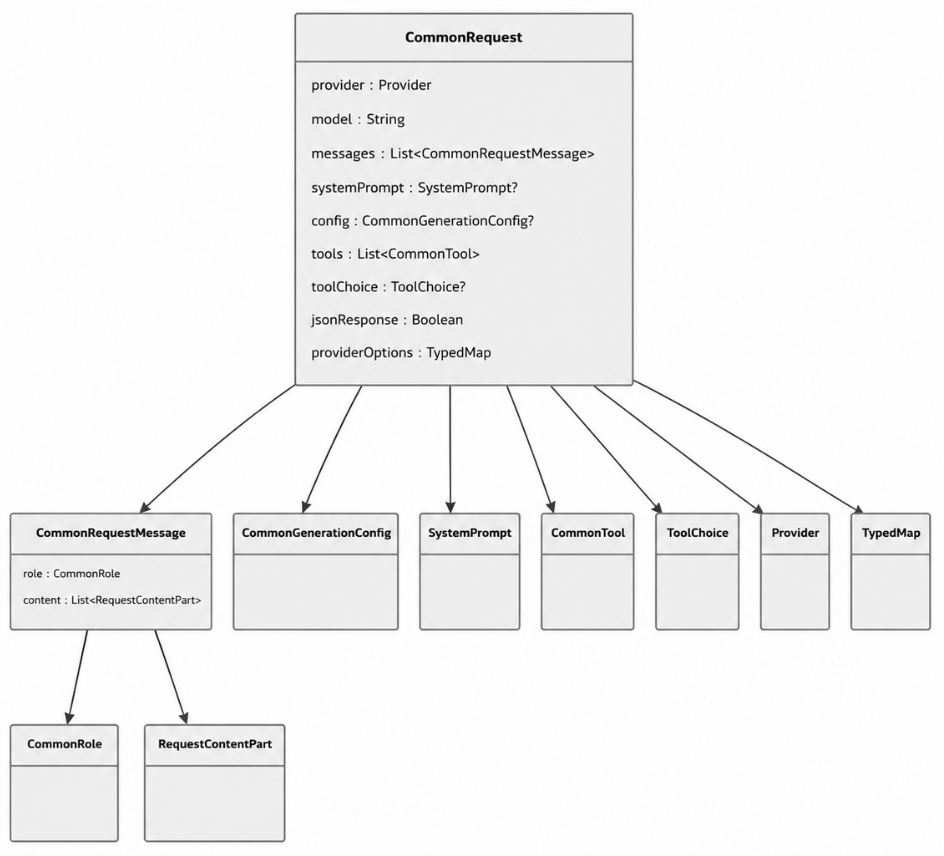
\includegraphics[width=0.95\textwidth]{../images/CommonRequestClasses}
        \caption{Estrutura de classes do \texttt{CommonRequest}.}
        \label{fig:commonrequest-classes}
    \end{figure}

    Para sistematizar a estrutura apresentada na Figura 3.2, a Tabela~\ref{tab:request-parametros} agrega todos os parâmetros relevantes do domínio de \textit{Request}, incluindo o objeto principal e os tipos diretamente associados. O objetivo é apresentar o significado funcional de cada campo no fluxo de construção do pedido.

    \begin{table}[H]
    \centering
    \footnotesize
    \setlength{\tabcolsep}{4pt}
    \renewcommand{\arraystretch}{1.15}
    \begin{tabularx}{\textwidth}{|>{\raggedright\arraybackslash}p{2.6cm}|>{\raggedright\arraybackslash}p{3.0cm}|>{\raggedright\arraybackslash}p{2.9cm}|>{\raggedright\arraybackslash}X|}
    \hline
    \textbf{Elemento} & \textbf{Campo} & \textbf{Tipo} & \textbf{Descrição} \\ \hline

    CommonRequest & provider & Provider & Fornecedor alvo da chamada. \\ \hline
    CommonRequest & model & String & Identificador do modelo a utilizar. \\ \hline
    CommonRequest & messages & \texttt{List\textless\allowbreak Common\allowbreak Request\allowbreak Message\textgreater} & Histórico de mensagens enviado ao modelo. \\ \hline
    CommonRequest & systemPrompt & SystemPrompt? & Prompt de sistema global (opcional). \\ \hline
    CommonRequest & config & CommonGenerationConfig? & Parâmetros de geração (opcional). \\ \hline
    CommonRequest & tools & \texttt{List\textless\allowbreak Common\allowbreak Tool\textgreater} & Ferramentas disponíveis para chamadas de função. \\ \hline
    CommonRequest & toolChoice & ToolChoice? & Política de seleção de ferramentas. \\ \hline
    CommonRequest & jsonResponse & Boolean & Indica se a resposta deve ser forçada a JSON. \\ \hline
    CommonRequest & providerOptions & TypedMap & Opções específicas do fornecedor. \\ \hline

    \texttt{Common\allowbreak Request\allowbreak Message} & role & CommonRole & Papel da mensagem (SYSTEM, USER, ASSISTANT, TOOL). \\ \hline
    \texttt{Common\allowbreak Request\allowbreak Message} & content & \texttt{List\textless\allowbreak Request\allowbreak Content\allowbreak Part\textgreater} & Conteúdo segmentado da mensagem. \\ \hline

    SystemPrompt & text & String & Conteúdo do prompt de sistema. \\ \hline

    \texttt{Common\allowbreak Generation\allowbreak Config} & temperature & Double? & Grau de aleatoriedade da geração. \\ \hline
    \texttt{Common\allowbreak Generation\allowbreak Config} & maxTokens & Int? & Limite máximo de tokens de saída. \\ \hline
    \texttt{Common\allowbreak Generation\allowbreak Config} & topP & Double? & Probabilidade cumulativa (nucleus sampling). \\ \hline
    \texttt{Common\allowbreak Generation\allowbreak Config} & stopSequences & \texttt{List\textless\allowbreak String\textgreater}? & Sequências que interrompem a geração. \\ \hline

    CommonTool & name & String & Nome da ferramenta. \\ \hline
    CommonTool & description & String & Descrição funcional da ferramenta. \\ \hline
    CommonTool & parametersSchema & JsonObjectMap & Esquema JSON dos parâmetros. \\ \hline

    ToolChoice & Auto/None/Required/Specific & -- & Estratégia de uso de ferramentas (auto, nenhuma, obrigatório ou lista específica). \\ \hline

    \texttt{Request\allowbreak Content\allowbreak Part} & TextPart & \texttt{text: String} & Conteúdo textual. \\ \hline
    \texttt{Request\allowbreak Content\allowbreak Part} & JsonPart & \texttt{json: JsonValue} & Conteúdo JSON estruturado. \\ \hline
    \texttt{Request\allowbreak Content\allowbreak Part} & ToolCallPart & \texttt{toolCallId, functionName, argumentsJson} & Chamada a ferramenta com argumentos. \\ \hline
    \texttt{Request\allowbreak Content\allowbreak Part} & ToolResultPart & \texttt{toolCallId, content} & Resultado de execução de ferramenta. \\ \hline

    \end{tabularx}
    \caption{Parâmetros do domínio de \textit{Request}.}
    \label{tab:request-parametros}
    \end{table}



    \subsection{{CommonResponse e CommonResponseEvent}}

    \chapter{Arquitetura e Desenho do Sistema}

    \section{Arquitetura Top-Level}
    A arquitetura top-level distingue claramente o produto principal desenvolvido, o \textbf{OmniAI SDK}, da aplicação de validação, a \textbf{OmniAI Gateway}. O SDK contém o domínio comum, os contratos, os adapters, o \textit{dispatcher}, a \textit{pipeline}, os \textit{interceptors}, a DSL de montagem e as abstrações de transporte. A OmniAI Gateway é um POC construído sobre esse SDK: carrega configuração, cria o grafo de componentes, instala os conectores Ktor e expõe endpoints HTTP compatíveis com os contratos estudados.

    \begin{figure}[H]
        \centering
        \begin{tikzpicture}[
            node distance=1.2cm and 1.5cm,
            box/.style={rectangle, draw, rounded corners, align=center, text width=3.8cm, minimum height=1.2cm, inner sep=5pt, thick},
            inner/.style={rectangle, draw, rounded corners, align=center, text width=4.2cm, minimum height=1.0cm, fill=white, inner sep=5pt, thick},
            sdk/.style={rectangle, draw, rounded corners, align=center, text width=4.2cm, minimum height=1.0cm, fill=gray!20, inner sep=5pt, thick},
            group/.style={rectangle, draw, rounded corners, dashed, inner sep=12pt},
            arrow/.style={-Latex, thick}
        ]
            % --- CLIENTES ---
            \node[box] (clients) {Clientes externos\\ex: REST Client, Claude Code};

            % --- OMNIAI GATEWAY (Grupo) ---
            \node[inner, right=1.5cm of clients, yshift=1.2cm] (config) {Configuração do POC \\ \texttt{application.conf}};
            \node[inner, below=0.5cm of config] (ktor) {Gateway Endpoints};
            \node[sdk, below=0.5cm of ktor] (sdk) {OmniAI SDK};

            % O grupo "fit" envolve os blocos internos
            \node[group, fit=(config)(ktor)(sdk), label={[align=center]above:\textbf{OmniAI Gateway POC}}] (gatewayGroup) {};

            % --- LADO DIREITO ---
            \node[box, right=1.5cm of ktor] (providers) {Fornecedores de inferência\\Gemini, Anthropic, OpenAI/Groq};
            \node[box, below=0.8cm of providers] (observability) {Operação local\\Logto, OTel, Prometheus/Grafana};

            % --- LIGAÇÕES ---
            % Entrada do grupo
            \draw[arrow] (clients.east) -- node[above, font=\footnotesize]{} (gatewayGroup.west);

            % Saída do grupo
            \draw[arrow] (gatewayGroup.east) -- node[above, font=\footnotesize]{} (providers.west);
            \draw[arrow] (gatewayGroup.east) -- (observability.west);

        \end{tikzpicture}
        \caption{Arquitetura top-level: POC OmniAI Gateway a instanciar e demonstrar o OmniAI SDK}
        \label{fig:top-level}
    \end{figure}

    \begin{figure}[H]
        \centering
        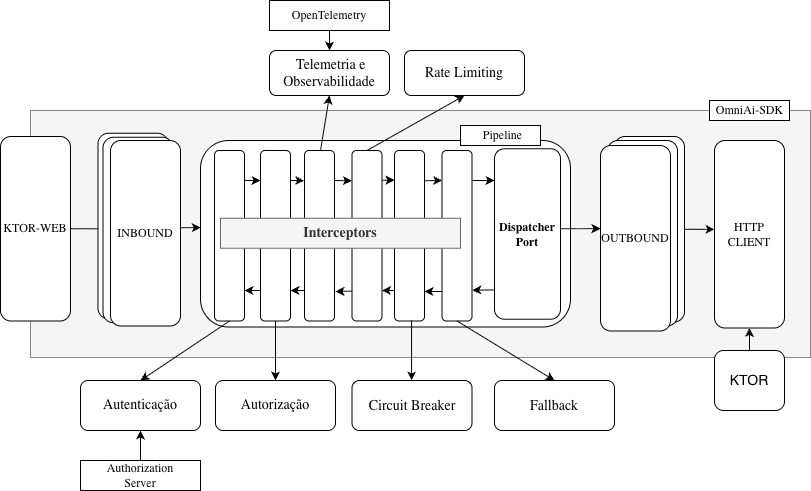
\includegraphics[width=0.95\textwidth]{../images/Arqui}
        \caption{Visão da integração entre Ktor, inbounds, pipeline, interceptors, outbounds e HTTP client no OmniAI SDK}
        \label{fig:arquitet-sdk}
    \end{figure}

    A Figura~\ref{fig:top-level} mostra que o POC não contém a lógica essencial de tradução, despacho ou resiliência. Essa lógica pertence ao SDK e é apenas instanciada pela aplicação final. A Figura~\ref{fig:arquitet-sdk} aproxima a visão interna: um conector HTTP recebe o corpo do pedido, converte-o para um DTO de contrato, invoca um \textit{inbound adapter}, e este chama um \texttt{DispatcherPort}. A partir desse ponto, a execução pode seguir por um dispatcher direto ou por um dispatcher apoiado numa \textit{pipeline}. No final, um \textit{outbound adapter} traduz o pedido comum para o contrato do fornecedor e utiliza um cliente HTTP abstrato para executar a chamada real.

    Esta organização permite que aplicações já compatíveis com APIs existentes possam ser integradas com esforço reduzido. Por exemplo, uma aplicação preparada para a API Anthropic pode alterar o seu \texttt{baseURL} para apontar para a OmniAI Gateway, mantendo o contrato esperado pelo cliente. O mesmo princípio aplica-se a clientes compatíveis com OpenAI e a cenários Gemini suportados pelo POC. A arquitetura foi também pensada para escalamento horizontal: o SDK evita estado global obrigatório, concentra estado transitório no contexto do pedido e define portas para substituir stores em memória por backends partilhados quando a Gateway é executada em múltiplas instâncias.

    \section{Arquitetura Hexagonal (Ports \& Adapters)}
    A Arquitetura Hexagonal foi escolhida para separar a lógica de domínio dos detalhes de transporte, dos contratos externos e das bibliotecas concretas. A formulação original de Cockburn descreve a aplicação no centro e os mecanismos externos ligados através de portas e adapters \cite{cockburn_hexagonal}. Esta abordagem é particularmente adequada a uma Gateway de IA, porque o sistema é dominado por integrações: clientes externos, APIs de fornecedores, servidores de autorização, telemetria e mecanismos de transporte.

    Uma alternativa seria uma arquitetura em camadas tradicional, com controladores, serviços e repositórios. Essa opção seria simples no início, mas tenderia a concentrar traduções de contratos, chamadas HTTP e regras operacionais no mesmo serviço de aplicação. Outra alternativa seria decompor cedo a solução em vários serviços independentes. Essa abordagem poderia escalar equipas e deploys, mas introduziria complexidade operacional excessiva para um SDK cujo objetivo principal é ser reutilizável dentro de diferentes aplicações. A opção hexagonal oferece um compromisso mais adequado: mantém uma estrutura modular e testável sem obrigar a transformar cada responsabilidade num serviço remoto. No contexto de gateways, esta separação também acompanha o padrão de API Gateway como camada de integração e política transversal \cite{api_gateway_design,ai_gateway_pattern,karl_ai_gateway}.

    \subsection{Contracts}
    Os módulos \texttt{contracts:openai}, \texttt{contracts:anthropic} e \texttt{contracts:gemini} modelam os formatos de pedido, resposta e eventos de cada fornecedor. Estes contratos são DTOs no sentido em que representam dados transportados na fronteira do sistema, mas não são apenas DTOs genéricos. São chamados \textit{contracts} porque codificam uma compatibilidade externa concreta: nomes de campos, estruturas JSON, eventos de \textit{streaming}, campos opcionais, formatos de erro e convenções específicas de cada API.

    Esta distinção é importante. Um DTO interno poderia ser livremente alterado sem impacto externo; um contrato compatível com OpenAI, Anthropic ou Gemini precisa de respeitar o formato que clientes e fornecedores esperam. Ao isolar estes contratos em módulos próprios, o SDK evita que detalhes como \texttt{tool\_calls}, \texttt{content\_block\_delta} ou \texttt{functionDeclarations} se espalhem pelo domínio comum.

    \subsection{Inbounds}
    Os \textit{inbound adapters} recebem pedidos no formato do cliente e traduzem-nos para \texttt{CommonRequest}. Cada inbound implementa a porta \texttt{InboundPort} e recebe um \texttt{DispatcherPort}, não uma implementação concreta de pipeline ou de fornecedor. Além disso, cada inbound usa uma implementação de \texttt{InboundTranslator}, responsável por converter o objeto de entrada para domínio e por converter a resposta comum de volta para o contrato do cliente.

    Esta decisão evita que o inbound exponha diretamente uma Web API. O SDK fornece adapters que trabalham sobre objetos de transferência, e a exposição HTTP fica noutro adapter, como o \texttt{gateway-ktor-server}. Assim, um servidor Ktor, uma função serverless, um handler Express ou outro mecanismo de entrada podem chamar o mesmo inbound desde que consigam construir o DTO esperado. Esta separação reduz a dependência do domínio e dos inbounds face a bibliotecas HTTP externas.

    \subsection{Outbounds}
    Os \textit{outbound adapters} fazem o caminho inverso: recebem um \texttt{CommonRequest}, traduzem-no para o contrato do fornecedor real e executam a chamada externa. Cada outbound implementa \texttt{OutboundPort}, identifica \texttt{provider}, \texttt{model} e \texttt{key}, e delega a tradução num \texttt{OutboundTranslator}. A implementação atual inclui outbounds para OpenAI, Anthropic e Gemini.

    Ao contrário dos inbounds, os outbounds precisam de comunicar com serviços externos. Por isso recebem uma implementação de \texttt{HttpTransportClient}. A implementação fornecida pelo SDK é baseada em Ktor, mas a porta permite substituir o transporte por outro cliente HTTP, por um mock em testes, por um cliente instrumentado ou por uma implementação específica de plataforma. Esta inversão de dependência é o que permite testar adapters sem depender de chamadas reais e evoluir o runtime sem reescrever o domínio.

    \subsection{Dispatcher}
    O \texttt{DispatcherPort} é a porta chamada pelos inbounds para executar um \texttt{CommonRequest}. A sua responsabilidade não é, por si só, conter inteligência de roteamento; é despachar o pedido para uma estratégia de execução. No SDK é fornecida uma implementação simples, criada por \texttt{routingDispatcherFactory}, que procura o outbound cujo \texttt{provider} e \texttt{model} correspondem aos campos do pedido e envia a chamada para esse adapter.

    Como se trata de uma interface, a arquitetura permite outras implementações com objetivos diferentes. Um consumidor do SDK pode fornecer um dispatcher direto, um dispatcher com seleção por custo, um dispatcher que consulta políticas externas ou um dispatcher que aplica regras mais complexas. A \textit{pipeline} fornecida pelo SDK é ela própria encaixada através de um adapter, \texttt{PipelineBackedDispatcher}, preservando a ideia de que os inbounds dependem apenas de \texttt{DispatcherPort}.

    \section{Ecossistema do SDK}
    O SDK está organizado como um projeto Gradle multi-módulo. Os módulos principais incluem \texttt{core}, \texttt{contracts}, \texttt{inbound}, \texttt{outbound}, \texttt{interceptors}, \texttt{mcp-broker}, \texttt{dispatcher}, \texttt{gateway-client}, \texttt{gateway-ktor-server} e \texttt{contracts:ktor-http}. Esta divisão permite evoluir cada área com responsabilidades claras: domínio e portas em \texttt{core}, contratos externos em \texttt{contracts}, adapters de entrada e saída em módulos próprios, preocupações transversais em \texttt{interceptors}, montagem declarativa em \texttt{gateway-client} e exposição HTTP/Ktor em \texttt{gateway-ktor-server}.

    O módulo \texttt{contracts:ktor-http} fornece a abstração de transporte \texttt{HttpTransportClient} e a implementação \texttt{KtorHttpTransportClient}. Esta camada encapsula chamadas HTTP, SSE, serialização, metadados de resposta, erros de rede e erros de parsing. Ao colocá-la atrás de uma interface, os outbounds não ficam presos a uma implementação específica de cliente HTTP.

    O módulo \texttt{gateway-client} disponibiliza uma DSL para montar uma Gateway. A aplicação consumidora pode declarar outbounds, interceptors, autenticação, autorização e modo de execução. A DSL permite escolher entre \texttt{useNativePipeline}, que monta a pipeline e o dispatcher padrão, e \texttt{useCustomDispatcher}, que permite substituir totalmente a estratégia de execução. Esta flexibilidade é essencial para um SDK: o POC usa a montagem nativa, mas outro consumidor pode querer um dispatcher próprio.

    A aplicação \texttt{OmniAiGateway} foi desenvolvida como POC de validação do SDK. O uso de \textit{composite build} do Gradle, através de \texttt{includeBuild("../OmniAi-SDK")} \cite{gradle_composite_builds}, não pretende simular a forma final de consumo em produção. A sua função foi acelerar o desenvolvimento do projeto final, permitindo compilar SDK e POC em conjunto, testar alterações imediatamente e evitar o ciclo pesado de publicar uma versão do SDK, atualizar dependências do POC e voltar a compilar. Numa distribuição real, a expectativa é que o SDK seja consumido como dependência versionada, nomeadamente via Maven para JVM e via NPM para Node.js/TypeScript.



    \chapter{Implementação e Evolução Técnica}

    \section{Stack Tecnológica e Metodologias}
    O \textbf{OmniAI SDK} foi desenvolvido em Kotlin Multiplatform \cite{kmp_ref} com targets JVM e JavaScript/Node.js. A escolha de KMP permite partilhar o domínio, os contratos, as portas, os adapters principais e parte da lógica geral entre plataformas, mantendo implementações específicas quando o ambiente o exige \cite{kotlin_multiplatform}. A serialização dos contratos é baseada em Kotlinx Serialization \cite{serialization_ref}, o que facilita a definição explícita dos modelos JSON estudados.

    O \textit{core} do \textbf{OmniAI SDK} é estritamente agnóstico em relação a \textit{frameworks} web e mecanismos de transporte HTTP. Contudo, para fornecer uma solução imediatamente utilizável, o projeto inclui módulos oficiais de integração baseados na \textit{framework} Ktor \cite{ktor_ref}. Estes módulos opcionais oferecem implementações de referência tanto para a execução de pedidos aos fornecedores (\textit{client-side}) como para a exposição das rotas da Gateway (\textit{server-side}). A \textbf{OmniAI Gateway} instanciada como Prova de Conceito (PoC) tira partido destas implementações prontas a usar. No entanto, a adoção do SDK não obriga ao uso do Ktor; a arquitetura garante que qualquer utilizador possa descartar estes módulos e implementar os adaptadores de rede utilizando a tecnologia da sua preferência, como o ecossistema Spring por exemplo, entre outros.

    As ferramentas de desenvolvimento incluíram Git, IntelliJ IDEA, o cliente HTTP do IDE para pedidos REST, Docker Compose para Logto \cite{logto_docs}, PostgreSQL \cite{postgresql_ref}, OpenTelemetry Collector \cite{opentelemetry_what_is}, Prometheus \cite{prometheus_ref} e Grafana \cite{grafana_ref}, além de clientes reais como Claude Code e SDKs oficiais dos fornecedores. Também foram usados assistentes de apoio, como Gemini no browser e agentes de programação como o Antigravity e Codex, para pesquisa, comparação de documentação e aceleração de tarefas, mantendo a validação no código, nos testes e nos cenários executados. Foi criada uma pipeline de \textbf{Continuous Integration} (CI) \cite{CI_ref}    existente executa \texttt{./gradlew clean build} como passo evolutivo, está prevista a criação de uma pipeline de \textbf{Continuous Deployment} (CD) para publicar as versões do nosso Software Development Kit,o \textbf{OmniAI SDK} em Maven e NPM.

    \section{A Primeira Iteração da Gateway}

    A primeira iteração do projeto consistiu numa Gateway HTTP construída diretamente, responsável por receber pedidos de clientes e encaminhá-los para fornecedores de inferência. Esta fase foi útil para validar rapidamente a viabilidade da solução, testar pedidos reais e compreender diferenças práticas entre as diferentes API's dos fornecedores, neste caso da OpenAI \cite{openai_api}, Anthropic\cite{anthropic_api} e Gemini\cite{google_gemini_api}.

    À medida que o sistema cresceu, essa abordagem revelou acoplamento excessivo. A tradução entre contratos, a configuração dos fornecedores, a autenticação, o tratamento de erros e o encaminhamento de pedidos começaram a concentrar-se na própria aplicação. Cada novo fornecedor ou preocupação exigia alterações no mesmo conjunto de componentes, tornando o código difícil de evoluir e de se testar.

A reorganização da arquitetura separou o produto principal, o \textbf{OmniAI SDK}, de uma aplicação final denominada \textbf{OmniAI Gateway}.
O \textbf{OmniAI SDK} passou a concentrar toda a lógica e abstrações reutilizáveis do domínio, incluindo contratos, portas e adaptadores (\textit{Ports \& Adapters}), o sistema de \textit{dispatching}, a \textit{pipeline} de execução, \textit{interceptors}, DSLs de configuração e abstrações HTTP multiplataforma. Desta forma, o SDK fornece toda a infraestrutura necessária para que qualquer utilizador consiga instanciar e configurar a sua própria \textbf{OmniAI Gateway}, adaptada ao seu contexto e necessidades.
A \textbf{OmniAI Gateway} representa, assim, uma aplicação concreta construída sobre o \textbf{OmniAI SDK}. No contexto deste projeto, foi desenvolvida uma \textbf{OmniAI Gateway} responsável por carregar configurações, instanciar os componentes necessários, instalar os conectores Ktor e expor \textit{endpoints} HTTP.

Esta aplicação tem como objetivo validar a arquitetura proposta e demonstrar que o \textbf{OmniAI SDK} permite construir \textit{gateways} funcionais, extensíveis e desacopladas dos diferentes fornecedores de modelos de IA. Assim, a \textbf{OmniAI Gateway} desenvolvida neste projeto atua como uma \textit{Proof of Concept} da abordagem arquitetural definida, servindo como exemplo prático da utilização do SDK.

Esta separação também influenciou o desenho da arquitetura para suportar escalamento horizontal. O \textbf{OmniAI SDK} foi projetado para manter o estado associado aos pedidos apenas em estruturas transitórias, como \texttt{GatewayContext} e \texttt{TypedMap}, expondo portas explícitas para componentes que necessitam de estado partilhado, como \textit{caches}, \textit{rate limiting}, \textit{circuit breakers}, autenticação e observabilidade.

Esta abordagem permite que uma instanciação simples de uma \textbf{OmniAI Gateway} utilize implementações em memória, reduzindo a complexidade inicial de configuração e execução. No entanto, em cenários de escalamento horizontal, esses mesmos mecanismos podem ser substituídos por sistemas distribuídos e partilhados, sem necessidade de alterações nos \textit{inbounds}, \textit{outbounds} ou contratos expostos pelo SDK.

Desta forma, o \textbf{OmniAI SDK} desacopla a lógica funcional da infraestrutura de persistência e sincronização, permitindo que diferentes implementações da \textbf{OmniAI Gateway} evoluam de ambientes locais e monolíticos para arquiteturas distribuídas de forma transparente.

\section{Decisões de Desenho e Alternativas Descartadas}

A análise de \textit{trade-offs} partiu de três critérios principais: preservar a estabilidade da versão demonstrável, manter o \textbf{OmniAI SDK} reutilizável e extensível independentemente da aplicação final e evitar que funcionalidades experimentais introduzissem acoplamento excessivo no domínio comum.

Neste contexto, importa recordar que a \textbf{OmniAI Gateway} apresentada neste projeto corresponde apenas a uma instanciação concreta construída sobre o \textbf{OmniAI SDK}. Assim, várias decisões arquiteturais foram tomadas não apenas a pensar na \textit{Proof of Concept}, mas sobretudo na preservação do SDK enquanto fundação reutilizável para futuras gateways, integrações e ambientes de execução.

As decisões seguintes não representam funcionalidades abandonadas, mas sim escolhas conscientes de âmbito para garantir que a primeira versão permanecesse estável, testável e arquiteturalmente coerente:

\begin{itemize}

\item \textbf{Geração de Bridges com KSP (Kotlin Symbol Processing):}
Foi ponderada a utilização de KSP para gerar automaticamente \textit{bridges} entre Kotlin e TypeScript/Node.js. Embora esta abordagem pudesse reduzir código manual na integração multiplataforma, implicaria lidar com configuração adicional, compatibilidade entre targets e diversos casos limite de tipagem entre Kotlin e JavaScript. Optou-se por uma fachada baseada em \texttt{@JsExport}, suficientemente controlada para expor o target JavaScript sem introduzir complexidade excessiva ou comprometer o prazo do projeto.

\item \textbf{Injeção Automática de Ferramentas via SSE:}
Também foi avaliada a possibilidade de a Gateway intercetar automaticamente \textit{tool calls} durante \textit{streams}, executar ferramentas e reinjetar os resultados no fluxo SSE de forma transparente para o cliente. Apesar de tecnicamente viável, esta funcionalidade exigiria mecanismos adicionais de gestão de estado conversacional, suspensão e retoma de streams, coordenação concorrente e normalização de diferenças entre fornecedores que emitem eventos distintos. A capacidade ficou identificada como evolução futura, mantendo a primeira versão focada nos elementos considerados essenciais: contratos comuns, adapters, pipeline de interceptors, segurança, observabilidade e resiliência.
\end{itemize}


\section{Evolução Arquitetural: De \textit{Inference Service} a \textit{Dispatcher}}

A primeira iteração da arquitetura concentrava comunicação, tradução de contratos e roteamento num componente designado por \texttt{InferenceService}. Embora esta abordagem tenha sido eficaz durante a fase inicial de desenvolvimento e prototipagem, rapidamente começou a aproximar-se de um \textit{God Object}: cada novo fornecedor, métrica, regra de segurança ou política de erro aumentava progressivamente a responsabilidade do mesmo serviço.

O problema principal não era apenas o crescimento do componente, mas sobretudo a direção das dependências. Ao conhecer diretamente contratos HTTP, clientes externos, regras de seleção de fornecedor e políticas transversais, o serviço tornava-se o ponto central de acoplamento da arquitetura. Qualquer alteração numa dessas áreas propagaria impacto para o núcleo do sistema, dificultando testes unitários, aumentando o custo de introdução de novos adapters e reduzindo significativamente o valor do SDK enquanto fundação reutilizável para diferentes gateways e cenários de execução.

A refatorização substituiu esse modelo por um contrato pequeno e explícito: o \texttt{DispatcherPort}. A responsabilidade do dispatcher passou a ser exclusivamente receber um \texttt{CommonRequest} e delegar a execução para uma estratégia de despacho. A implementação padrão fornecida pelo SDK, criada através de \texttt{routingDispatcherFactory}, realiza um roteamento simples baseado no fornecedor e no modelo presentes no pedido. Contudo, por se tratar apenas de uma interface, o SDK não impõe esta estratégia: qualquer consumidor pode substituir o dispatcher por outra implementação sem necessidade de alterar inbounds, contratos ou adapters existentes.

Esta alteração teve impacto direto na modularidade da arquitetura. Os inbounds passaram a depender apenas da porta \texttt{DispatcherPort}; os outbounds ficaram responsáveis exclusivamente pela tradução de contratos e comunicação externa; e as preocupações transversais foram deslocadas para a \textit{pipeline} de interceptors. Como consequência, a \texttt{OmniAiGateway} deixou de representar uma implementação rigidamente acoplada à infraestrutura interna e passou a funcionar como uma composição configurável construída sobre o \textbf{OmniAI SDK}.

Na prática, esta separação permitiu preservar o SDK como uma fundação independente do \textit{Proof of Concept}, reutilizável na construção de outras gateways, runtimes ou integrações futuras. A \texttt{OmniAiGateway} desenvolvida neste projeto representa, assim, apenas uma configuração concreta dessa infraestrutura arquitetural, utilizada para validar a abordagem proposta e demonstrar a viabilidade do modelo definido.

    \section{Implementação da Camada HTTP: \texttt{gateway-ktor-server}}
    \label{sec:gateway-ktor-server}

    A camada de exposição HTTP da Gateway é implementada no módulo \texttt{gateway-ktor-server}. Este módulo estabelece a ponte entre o servidor web (Ktor) e os \textit{inbound adapters} do domínio, garantindo que o núcleo do sistema permanece agnóstico em relação à tecnologia de transporte de entrada.

    A implementação baseia-se num padrão de conectores (\texttt{InboundConnector}) que regista rotas específicas para cada contrato suportado. O módulo expõe três funções de extensão sobre a interface de encaminhamento (\texttt{Route}) do Ktor:

    \begin{table}[H]
        \centering
        \footnotesize
        \renewcommand{\arraystretch}{1.25}
        \begin{tabularx}{\textwidth}{|>{\raggedright\arraybackslash}p{3.5cm}|>{\raggedright\arraybackslash}p{4cm}|Y|}
            \hline
            \textbf{Conector Ktor} & \textbf{Caminho (Path) Predefinido} & \textbf{DTOs de Contrato (Pedido / Resposta)} \\
            \hline
            \texttt{openAiConnector()} & \texttt{/v1/chat/completions} & \texttt{OpenAiChatCompletionsRequest} / \texttt{OpenAiChatCompletionsResponse} \\
            \hline
            \texttt{anthropicConnector()} & \texttt{/v1/messages} & \texttt{AnthropicMessagesRequest} / \texttt{AnthropicMessageResponse} \\
            \hline
            \texttt{geminiConnector()} & \texttt{/v1beta/models/\{model\}:generateContent} & \texttt{GeminiGenerateContentRequest} / \texttt{GeminiGenerateContentResponse} \\
            \hline
        \end{tabularx}
        \caption{Conectores HTTP disponibilizados pela Gateway Ktor}
        \label{tab:ktor-connectors}
    \end{table}

    A ligação entre a rota HTTP e a porta de entrada opera num ciclo de duas fases. Numa primeira fase, as rotas são registadas e aguardam a injeção da dependência. Quando o servidor é iniciado, o \textit{adapter} concreto (por exemplo, \texttt{OpenAiInboundAdapter}) é injetado no conector através da função \texttt{connect()}.
    
    O fluxo de processamento de um pedido HTTP obedece sempre à mesma sequência:
    \begin{enumerate}
        \item \textbf{Desserialização:} O corpo do pedido HTTP é convertido para o DTO do contrato correspondente (e.g., \texttt{OpenAiChatCompletionsRequest}), devolvendo um erro \texttt{400 Bad Request} em caso de falha sintática.
        \item \textbf{Extração de Metadados:} Atributos essenciais do protocolo HTTP são extraídos e propagados para a \texttt{TypedMap} do contexto interno. A configuração \texttt{defaultKtorRequestMetadataBinder} processa o cabeçalho \texttt{Authorization} (removendo o prefixo \texttt{Bearer}), resolve o endereço IP do cliente (verificando \texttt{X-Forwarded-For} e \texttt{X-Real-IP}) e mapeia parâmetros de rota, como o modelo dinâmico na API do Gemini.
        \item \textbf{Execução e \textit{Streaming}:} O conector avalia se o cliente solicitou \textit{streaming} (através de \textit{flags} no corpo do pedido ou parâmetros \textit{query}). Consoante o caso, delega a execução para o método \texttt{generate()} (síncrono) ou \texttt{generateStream()} da respetiva porta.
       \item \textbf{Resposta:} Os resultados unários são diretamente serializados para JSON. Em contraste, as respostas em \textit{streaming} originam um \texttt{Flow} reativo, onde cada evento emitido é individualmente serializado em JSON e transmitido de forma progressiva ao cliente através de \textit{Server-Sent Events} (SSE).
    \end{enumerate}

    \section{Implementação do HttpTransportClient em Ktor}
    \label{sec:ktor-transport-impl}

    A abstração de chamadas HTTP de saída é garantida pela interface \texttt{HttpTransportClient}, descrita na Secção~\ref{subsec:http-transport-client}. A implementação concreta fornecida pelo \textit{SDK}, \texttt{KtorHttpTransportClient}, assenta no cliente HTTP Ktor e reside no módulo \texttt{contracts:ktor-http}. 
    
    Esta implementação suporta retentativas configuráveis com atraso temporal entre tentativas (\textit{delay}), tratamento explícito de exceções de rede (traduzidas para \texttt{NetworkError}) e falhas de \textit{parsing} de JSON (traduzidas para \texttt{SerializationError}). Suporta ainda a integração transparente com o \textit{plugin} nativo de SSE do Ktor para o consumo de respostas progressivas.

    A configuração do cliente subjacente é centralizada em \texttt{PlatformHttpClient}, que padroniza tempos limite (\textit{timeouts}) de ligação e \textit{socket}, bem como o processo de \textit{Content Negotiation}. Um aspeto fulcral desta organização é o facto de a configuração base ser resolvida por implementações específicas de plataforma (JVM ou JavaScript). Isto permite ao \textit{SDK} funcionar corretamente como biblioteca \textit{Kotlin Multiplatform}.

Esta arquitetura permite adaptar o comportamento da camada HTTP ao contexto de execução sem alterar os adapters dos fornecedores. Durante os testes, por exemplo, os \textit{outbounds} podem comunicar com implementações fictícias em memória, evitando dependências de rede externa. Já em ambientes produtivos, a implementação base pode ser substituída por variantes com características específicas definidas pelo consumidor do \textbf{OmniAI SDK}, mantendo inalterada a lógica de abstração e tradução dos contratos dos diferentes fornecedores de Inteligência Artificial.



    \section{Implementações Inbound e Outbound}
    \label{sec:inbounds-outbounds}
    
    O coração lógico da OmniAI Gateway materializa-se nos \textit{adapters} de entrada (\textit{inbounds}) e saída (\textit{outbounds}). Cada \textit{adapter} é rigorosamente desenhado em torno do padrão Porta-Adaptador e apoiado num \textit{Translator} dedicado. Esta separação permite que a realização do pedido e o mapeamento físico de atributos JSON vivam em componentes distintos, facilitando testes isolados. A Figura~\ref{fig:translator-arch} ilustra a arquitetura base de tradução.
 \begin{figure}[H]
    \centering
    \resizebox{\textwidth}{!}{%
    \begin{tikzpicture}[
        node distance=1.2cm and 2.8cm,
        % Estilos das caixas
        box/.style={rectangle, rounded corners=3pt, draw=black!60, thick, minimum width=3.8cm, minimum height=1cm, align=center, font=\sffamily\footnotesize},
        % Aumentei ligeiramente a altura do basebox para 1.4cm para as setas não baterem nas bordas
        basebox/.style={box, fill=black!70, text=white, minimum height=1.4cm, font=\sffamily\footnotesize\bfseries}, 
        implbox/.style={box, fill=gray!10, text=black},
        domainbox/.style={box, fill=white, draw=gray!80, minimum width=4.5cm, minimum height=1.3cm, font=\sffamily\small\bfseries},
        domainbg/.style={rectangle, rounded corners=5pt, fill=gray!5, draw=gray!50, dashed, thick, inner sep=8pt},
        % Estilos das setas
        flowarrow/.style={-{Stealth[length=2.5mm]}, thick, draw=black!80},
        inheritarrow/.style={-{Triangle[open, length=3mm, width=3mm]}, thick, draw=gray!70, dashed},
        % Estilo dos rótulos
        lbl/.style={fill=white, inner sep=3pt, font=\sffamily\scriptsize, text=black!80, draw=gray!30, very thin, rounded corners=2pt}
    ]

    % Central Domain Objects
    \node[domainbox] (req) {Common Request};
    \node[domainbox, below=1.2cm of req] (res) {Common Response};
    \node[domainbox, below=1.2cm of res] (event) {Common Response Event};
    
    % Domain Background
    \node[domainbg, fit=(req) (res) (event)] (domaingroup) {};
    % Redesenhar as caixas para ficarem sobre o fundo
    \node[domainbox] (req) at (req) {Common Request};
    \node[domainbox] (res) at (res) {Common Response};
    \node[domainbox] (event) at (event) {Common Response Event};
    
    % Título do Domínio Comum
    \node[font=\sffamily\footnotesize\bfseries, text=black!70, anchor=south] at ([yshift=0.15cm]domaingroup.north) {DOMÍNIO COMUM};

    % Left Side: Inbound
    \node[basebox, left=2.8cm of req] (inbase) {Inbound Translator};
    \node[implbox, below=1.2cm of inbase] (inanth) {Anthropic Inbound\\Translator};
    \node[implbox, below=0.6cm of inanth] (ingem) {Gemini Inbound\\Translator};
    \node[implbox, below=0.6cm of ingem] (inoai) {OpenAi Inbound\\Translator};

    % Left hierarchy arrows
    \draw[thick, dashed, draw=gray!70] (inoai.west) -- ++(-0.5,0) coordinate (in_bus);
    \draw[thick, dashed, draw=gray!70] (ingem.west) -- (ingem.west -| in_bus);
    \draw[thick, dashed, draw=gray!70] (inanth.west) -- (inanth.west -| in_bus);
    \draw[inheritarrow] (in_bus) |- (inbase.west);

    % Right Side: Outbound
    \node[basebox, right=2.8cm of req] (outbase) {Outbound Translator};
    \node[implbox, below=1.2cm of outbase] (outanth) {Anthropic Outbound\\Translator};
    \node[implbox, below=0.6cm of outanth] (outgem) {Gemini Outbound\\Translator};
    \node[implbox, below=0.6cm of outgem] (outoai) {OpenAi Outbound\\Translator};

    % Right hierarchy arrows
    \draw[thick, dashed, draw=gray!70] (outoai.east) -- ++(0.5,0) coordinate (out_bus);
    \draw[thick, dashed, draw=gray!70] (outgem.east) -- (outgem.east -| out_bus);
    \draw[thick, dashed, draw=gray!70] (outanth.east) -- (outanth.east -| out_bus);
    \draw[inheritarrow] (out_bus) |- (outbase.east);
    
    % ==========================================
    % Fluxos de Dados Inbound
    % ==========================================
    % Linha reta perfeita e centrada
    \draw[flowarrow] ([yshift=12pt]inbase.east) -- node[lbl] {toDomain()} ([yshift=12pt]req.west);
    
    % Linhas paralelas (sem declive) usando a sintaxe |--
    % Rótulo mais à esquerda (centrado no primeiro segmento), ligeiramente para cima e direita
    \draw[flowarrow] (res.west) -- node[lbl, above, yshift=20pt, xshift=0pt] {fromDomain()} ++(-1.4,0) |- ([yshift=-2pt]inbase.east);
    
    % Rótulo centrado no segmento, para cima e direita
    \draw[flowarrow] (event.west) -- node[lbl, above, yshift=20pt] {fromDomainEvent()} ++(-2.0,0) |- ([yshift=-15pt]inbase.east);

    % ==========================================
    % Fluxos de Dados Outbound
    % ==========================================
    % Linha reta perfeita e centrada
    \draw[flowarrow] ([yshift=12pt]req.east) -- node[lbl] {fromDomain()} ([yshift=12pt]outbase.west);
    
    % Linhas paralelas garantidas sem declive.
    % O ToDomain fica no primeiro segmento saindo do Outbase, movendo-o efetivamente mais para a direita.
    \draw[flowarrow] ([yshift=-2pt]outbase.west) -- node[lbl,left, xshift=-11pt, yshift=-35pt] {toDomain()} ++(-1.4,0) |- (res.east);
    
    % O toDomainEvent ajustado ligeiramente para cima
    \draw[flowarrow] ([yshift=-15pt]outbase.west) -- node[lbl, left, yshift=-100pt, xshift=-9pt] {toDomainEvent()} ++(-1.0,0) |- (event.east);

    \end{tikzpicture}%
    }
    \caption{Arquitetura de Tradução e Fluxo de Dados entre Contratos e Domínio Comum}
    \label{fig:translator-arch}
\end{figure}

    \section{Translators de Entrada (Inbound)}

    Os \textit{Inbound Translators} implementam a conversão do pedido original de um cliente, de uma resposta completa, e de eventos intermédios em \textit{streaming} originários do domínio para a semântica do cliente.

    \subsection{OpenAI Inbound Translator}

    A implementação \texttt{OpenAiInboundTranslator} processa pedidos conformes à sintaxe da OpenAI.
    
\begin{table}[H]
    \centering
    \footnotesize
    \renewcommand{\arraystretch}{1.25}
    \begin{tabularx}{\textwidth}{|>{\ttfamily\raggedright\arraybackslash}p{4cm}|Y|}
        \hline
        \textbf{Contrato Inbound (OpenAI)} & \textbf{Mapeamento para CommonRequest} \\
        \hline
        temperature, maxTokens, topP & Integrados na \texttt{CommonGenerationConfig}. O \texttt{model} é mapeado diretamente no nível superior do \texttt{CommonRequest}. \\
        \hline
        stop & Resolvedor distingue entre \texttt{Single} e \texttt{Multiple} e produz \texttt{List<String>}. \\
        \hline
        messages[].role & Traduzido estritamente para \texttt{SYSTEM}, \texttt{ASSISTANT}, \texttt{TOOL}, \texttt{USER} (padrão se omisso). \\
        \hline
        messages[].content \& toolCalls & Content gera \texttt{TextPart}. Chamadas de ferramenta geram \texttt{ToolCallPart(toolCallId, functionName)} com os argumentos encapsulados num mapa sob a chave "raw". Se o papel for \texttt{TOOL}, gera \texttt{ToolResultPart} convertendo o texto para primitivas JSON. \\
        \hline
        tools[].function & \texttt{CommonTool(name, description, parametersSchema)} extraindo as propriedades do schema. \\
        \hline
        toolChoice & Resolve de \texttt{auto/none/required} para \texttt{ToolChoice.Auto/None/Required}, ou resolve a chamada específica de função. \\
        \hline
        responseFormat & Avalia \texttt{type == "json\_object"} ou \texttt{"json\_schema"} como \texttt{jsonResponse = true}. \\
        \hline
        stream, frequencyPenalty, presencePenalty, n, seed, user, logitBias, logProbs, topLogProbs & Colocados na \texttt{TypedMap} (\texttt{providerOptions}) do \texttt{CommonRequest}, servindo como opções específicas não abrangidas pelo domínio comum. \\
        \hline
    \end{tabularx}
\caption{Mapeamento Inbound: OpenAI Request para Domínio}
\end{table}

\begin{table}[H]
    \centering
    \footnotesize
    \renewcommand{\arraystretch}{1.25}
    \begin{tabularx}{\textwidth}{|>{\ttfamily\raggedright\arraybackslash}p{4cm}|Y|}
        \hline
        \textbf{Domínio Comum} & \textbf{Mapeamento para Contrato Resposta (OpenAI)} \\
        \hline
        id \& created & Utiliza o \texttt{id} nativo ou gera um UUID \texttt{chatcmpl-...}. O tempo é recuperado das \texttt{providerOptions} ou gerado pelo \texttt{Clock.System}. \\
        \hline
        choices[].message.content & O conteúdo é destilado via \texttt{firstRenderableContentOrNull()} que privilegia o primeiro \texttt{TextPart}, caindo em \texttt{RefusalPart} ou representação string de \texttt{JsonPart}. \\
        \hline
        choices[].message
        .toolCalls & Um \texttt{ToolCallPart} origina um \texttt{OpenAiToolCallOutput} formatando os \texttt{argumentsJson} num string unificado. \\
        \hline
        choices[].finishReason & Traduz \texttt{STOP -> stop}, \texttt{LENGTH -> length}, \texttt{TOOL\_CALL -> tool\_calls}, \texttt{CONTENT\_FILTER -> content\_filter}. \\
        \hline
        usage & Mapeia \texttt{inputTokens}, \texttt{outputTokens} e \texttt{totalTokens} para \texttt{promptTokens}, \texttt{completionTokens} e \texttt{totalTokens}, respetivamente. \\
        \hline
    \end{tabularx}
\caption{Mapeamento Inbound: Domínio para OpenAI Response Unária}
\end{table}

\begin{table}[H]
    \centering
    \footnotesize
    \renewcommand{\arraystretch}{1.25}
    \begin{tabularx}{\textwidth}{|>{\raggedright\arraybackslash}p{4cm}|Y|}
        \hline
        \textbf{Common Response Event} & \textbf{Mapeamento para Stream Chunk (OpenAI)} \\
        \hline
        \texttt{ResponseStarted} & Emite Chunk inicial. \texttt{choices} ficam vazias. \\
        \hline
        \texttt{ChoiceStarted} & Emite Chunk com índice da \textit{choice}. O \texttt{delta} contém apenas a definição do \texttt{role} (\textit{assistant}). \\
        \hline
        \texttt{TextDeltaEvent} & Emite Chunk com \texttt{delta.content} preenchido pelo texto. \\
        \hline
        \texttt{ToolCallStartedEvent} & Emite Chunk inicializando o delta de \texttt{toolCalls}: define o \texttt{id}, a \texttt{type="function"} e o nome da função (\texttt{arguments=""}). \\
        \hline
        \texttt{ToolCallArguments
        DeltaEvent} & Emite Chunk contendo fragmentos incrementais em \texttt{function.arguments}. O nome da função é omitido neste pacote. \\
        \hline
        \texttt{ChoiceFinished} & Emite Chunk apenas com a tradução do \texttt{finishReason}. \texttt{delta} vai vazio. \\
        \hline
        \texttt{UsageReported} & Emite Chunk especial sem \textit{choices}, transportando o objeto global \texttt{usage}. \\
        \hline
        \texttt{ResponseCompleted} & Emite Chunk sem \textit{choices}, sinalizando a conclusão bem-sucedida do stream. \\
        \hline
        \texttt{ResponseErrored} & Emite Chunk injetando a mensagem de erro como texto no \texttt{delta.content} (simplificação face ao formato de erro nativo SSE da OpenAI). \\
        \hline
    \end{tabularx}
\caption{Mapeamento Inbound: Domínio para OpenAI Streaming (\texttt{fromDomainEvent})}
\end{table}

\subsection{Anthropic Inbound Translator}

A integração de entrada da Anthropic converte requisições que utilizam a sintaxe \textit{Messages API}.


\begin{table}[H]
    \centering
    \footnotesize
    \renewcommand{\arraystretch}{1.25}
    \begin{tabularx}{\textwidth}{|>{\ttfamily\raggedright\arraybackslash}p{4.5cm}|Y|}
        \hline
        \textbf{Contrato Inbound (Anthropic)} & \textbf{Mapeamento para CommonRequest} \\
        \hline
        temperature, maxTokens, topP, stopSequences & Integrados na \texttt{CommonGenerationConfig}. O \texttt{model} é mapeado diretamente no nível superior do \texttt{CommonRequest}. \\
        \hline
        system & A matriz de \texttt{AnthropicContent} converte \texttt{ListContentBlock} em \texttt{SystemPrompt} através da concatenação estrita de nós textuais via \texttt{joinToString()}. É ignorado se estiver em branco. \\
        \hline
        messages[].role & Convertido estritamente para os enumerados \texttt{SYSTEM}, \texttt{ASSISTANT}, \texttt{TOOL}, \texttt{USER}. \\
        \hline
        messages[].content & \texttt{Text} gera \texttt{TextPart}. \texttt{ToolUse} gera \texttt{ToolCallPart(id, name, input)}, com fallback automático para o ID (\texttt{"anthropic-tool-use-\$index"}). \texttt{ToolResult} injeta num \texttt{ToolResultPart}. \textbf{Nota}: Nós \texttt{Thinking} (raciocínio interno) presentes no input são descartados e devolvem \texttt{null}. \\
        \hline
        tools & Lista mapeada para \texttt{CommonTool}. O \texttt{inputSchema} é promovido para um \texttt{JsonObject} universal no campo \texttt{parametersSchema}. \\
        \hline
        toolChoice & Traduz estritamente \texttt{auto -> Auto}, \texttt{none -> None}, \texttt{any -> Required}, e instâncias \texttt{tool -> Specific(name)}. \\
        \hline
        \normalfont\textit{(Constantes da Integração)} & O campo \texttt{provider} é fixado como \texttt{Provider.ANTHROPIC} e \texttt{jsonResponse} como \texttt{false}. \\
        \hline
        stream, topK, stopToken, thinking, metadata & Opções específicas avançadas transferidas para a \texttt{TypedMap} (\texttt{providerOptions}) do \texttt{CommonRequest}. \\
        \hline
    \end{tabularx}
    \caption{Mapeamento Inbound: Anthropic Request para Dominio}
\end{table}

Na resposta unária (\texttt{fromDomain}), a conversão reverte a abstração semântica para a estrutura \texttt{AnthropicMessageResponse}, forçando o papel nativo para \texttt{"assistant"}.

\begin{table}[H]
    \centering
    \footnotesize
    \renewcommand{\arraystretch}{1.25}
    \begin{tabularx}{\textwidth}{|>{\ttfamily\raggedright\arraybackslash}p{4cm}|Y|}
        \hline
        \textbf{Domínio Comum} & \textbf{Mapeamento para Contrato Resposta (Anthropic)} \\
        \hline
        id \& model & Utiliza diretamente os valores de \texttt{id} e \texttt{model} da \texttt{CommonResponse}. \\
        \hline
        choices[].message.role & Convertido de \texttt{CommonRole} para \texttt{assistant} (na prática, mapeia \texttt{SYSTEM}, \texttt{ASSISTANT} e \texttt{TOOL} para \texttt{assistant}). \\
        \hline
        choices[].message.content & O conteúdo é destilado preservando os elementos nativos: \texttt{TextPart} gera texto, \texttt{ToolCallPart} origina \texttt{ToolUse} preservando a hierarquia do JSON interno, \texttt{JsonPart} é traduzido via \texttt{toString()} para texto, e os \texttt{RefusalPart} são totalmente ignorados e omitidos do mapeamento. \\
        \hline
        choices[].finishReason & Convertido estritamente para \texttt{end\_turn}, \texttt{max\_tokens}, \texttt{tool\_use} e \texttt{stop\_sequence}. \\
        \hline
        usage & Mapeado para o correspondente \texttt{AnthropicUsage} (\texttt{inputTokens} e \texttt{outputTokens}). \\
        \hline
    \end{tabularx}
\caption{Mapeamento Inbound: Domínio para Anthropic Message Response Unária}
\end{table}

No fluxo reativo (\textit{Server-Sent Events} - SSE), a abstração emite os eventos específicos documentados pela Anthropic.

\begin{table}[H]
    \centering
    \footnotesize
    \renewcommand{\arraystretch}{1.25}
    \begin{tabularx}{\textwidth}{|>{\raggedright\arraybackslash}p{4.5cm}|Y|}
        \hline
        \textbf{Common Response Event} & \textbf{Mapeamento para Evento SSE (Anthropic)} \\
        \hline
        \texttt{ResponseStarted} & Devolve \texttt{MessageStart} com metadados estáticos e \texttt{role="assistant"}. \\
        \hline
        \texttt{ChoiceStarted} & Devolve \texttt{ContentBlockStart} com o índice da \textit{choice}, anunciando um bloco de \texttt{Text}. \\
        \hline
        \texttt{TextDeltaEvent} & Traduz o \texttt{text} nativamente para o evento SSE \texttt{ContentBlockDelta(TextDelta)}. \\
        \hline
        \texttt{ToolCallStartedEvent} & Inicia um bloco via \texttt{ContentBlockStart(ToolUse)}, preservando o \texttt{id} e \texttt{name} e injetando um \texttt{JsonObject} vazio. \\
        \hline
        \texttt{ToolCallArgumentsDeltaEvent}& Transmite fragmentos parciais de argumentos delegando num SSE \texttt{ContentBlockDelta(InputJsonDelta)}. \\
        \hline
        \texttt{ChoiceFinished} & Emite o evento SSE \texttt{MessageDelta} contendo a sumarização convertida para \texttt{stopReason}. \\
        \hline
        \texttt{UsageReported} & Emite o evento SSE \texttt{MessageDelta} informando a sumarização de tokens processados. \\
        \hline
        \texttt{ResponseCompleted} & Emite o evento de fecho de fluxo \texttt{MessageStop}. \\
        \hline
        \texttt{ResponseErrored} & Interrompe a \textit{stream} enviando um evento \texttt{Error}, distinguindo falhas transitórias via tipo \texttt{overloaded\_error} vs \texttt{api\_error}. \\
        \hline
    \end{tabularx}
    \caption{Mapeamento Inbound: Eventos SSE Anthropic (\texttt{fromDomainEvent})}
\end{table}

    \subsection{Gemini Inbound Translator}

    A camada de tradução de entrada para a API Gemini normaliza as assimetrias da abstração de objetos \texttt{GenerateContent}.

    \begin{table}[H]
        \centering
        \footnotesize
        \renewcommand{\arraystretch}{1.25}
        \begin{tabularx}{\textwidth}{|>{\ttfamily\raggedright\arraybackslash}p{4.5cm}|Y|}
            \hline
            \textbf{Contrato Inbound (Gemini)} & \textbf{Mapeamento para CommonRequest} \\
            \hline
            generationConfig & Propriedades base (\texttt{temperature}, \texttt{topP}, \texttt{stopSequences}) extraídas para a \texttt{CommonGenerationConfig}. \\
            \hline
            model & Identificador extraído do \textit{path} HTTP. Em caso de ausência absoluta aplica o \textit{fallback} de constante \texttt{"NO MODEL"}. \\
            \hline
            systemInstruction & Transposto para \texttt{SystemPrompt} unindo as \texttt{parts} de texto disponíveis num único bloco com separação de linha. \\
            \hline
            contents[].role & Mapeia papéis convertendo \texttt{model} ou \texttt{assistant} $\rightarrow$ \texttt{ASSISTANT}, \texttt{function} $\rightarrow$ \texttt{TOOL}, e mantendo \texttt{user}. \\
            \hline
            contents[].parts & \texttt{text} gera \texttt{TextPart}. \texttt{functionCall} gera \texttt{ToolCallPart}. \texttt{functionResponse} gera \texttt{ToolResultPart}. \\
            \hline
            tools[].functionDeclarations & Realiza o \textit{flattening} da hierarquia (\texttt{tools -> functionDeclarations}) para nivelar numa única \texttt{List<CommonTool>}. \\
            \hline
            toolConfig.functionCallingConfig & Mapeia \texttt{mode} (ex: \texttt{auto -> Auto}, \texttt{any -> Required}) e converte chamadas permitidas em escolhas específicas. \\
            \hline
            generationConfig.responseMimeType & Infere \texttt{jsonResponse = true} se for \texttt{application/json} ou se existir explicitamente um \texttt{responseJsonSchema}. \\
            \hline
            topK, thinkingConfig & Opções específicas avançadas transferidas para a \texttt{TypedMap} (\texttt{providerOptions}) do \texttt{CommonRequest}. \\
            \hline
        \end{tabularx}
        \caption{Mapeamento Inbound: Gemini Request}
    \end{table}

    De modo recíproco, no mapeamento da resposta unária (\texttt{fromDomain}), os objetos de domínio são transportados para a gramática altamente tipada das \texttt{GeminiGenerateContentResponse}.

    \begin{table}[H]
        \centering
        \footnotesize
        \renewcommand{\arraystretch}{1.25}
        \begin{tabularx}{\textwidth}{|>{\ttfamily\raggedright\arraybackslash}p{4cm}|Y|}
            \hline
            \textbf{Domínio Comum} & \textbf{Mapeamento para Contrato Resposta (Gemini)} \\
            \hline
            id \& model & Copiados diretamente para \texttt{responseId} e \texttt{modelVersion}. \\
            \hline
            choices & Geram os respetivos \texttt{GeminiCandidate}, acoplando o índice e revertendo a hierarquia de papéis (\texttt{SYSTEM/ASSISTANT -> "model"}, \texttt{TOOL -> "function"}, \texttt{USER -> "user"}). \\
            \hline
            choices[].message.content & De forma simétrica, processa \texttt{TextPart} gerando os campos textuais de um \texttt{GeminiResponsePart}, instancia o nó de propriedades no caso dos \texttt{ToolCallPart}, converte \texttt{JsonPart} como uma literal \texttt{String} em texto JSON e reverte os \texttt{RefusalPart} apresentando a razão recusa da geração de conteúdo. \\
            \hline
            choices[].finishReason & Transposto restritamente para as constantes enumeradas \texttt{STOP}, \texttt{MAX\_TOKENS} e \texttt{SAFETY}. \\
            \hline
            usage & Compacta e renomeia contadores de abstração para a estrutura dimensional \texttt{GeminiUsageMetadata} (\texttt{promptTokenCount}, \texttt{candidatesTokenCount}). \\
            \hline
        \end{tabularx}
        \caption{Mapeamento Inbound: Domínio para Gemini Generate Content Response Unária}
    \end{table}

    No fluxo de \textit{streaming} via Server-Sent Events (SSE), a API do Gemini distingue-se por não possuir objetos dedicados a deltas parciais (ao contrário da OpenAI ou Anthropic). Em vez disso, a Google reutiliza o mesmo objeto estrutural completo da resposta unária (\texttt{GeminiGenerateContentResponse}) para encapsular cada fragmento progressivo da \textit{stream}. Consequentemente, o tradutor é forçado a mapear os deltas granulares de domínio (\texttt{CommonResponseEvent}) recriando exaustivamente a hierarquia profunda do DTO nativo para cada evento emitido (instanciando \texttt{candidates}, \texttt{content} e \texttt{parts} até mesmo para transmitir apenas uma simples \textit{string} parcial).

    \begin{table}[H]
        \centering
        \footnotesize
        \renewcommand{\arraystretch}{1.25}
        \begin{tabularx}{\textwidth}{|>{\raggedright\arraybackslash}p{4cm}|Y|}
            \hline
            \textbf{Common Response Event} & \textbf{Mapeamento para Evento SSE (Gemini Chunk)} \\
            \hline
            \texttt{ResponseStarted} & Emite uma instância básica portadora exclusivamente de metadados como o \texttt{modelVersion} e \texttt{responseId}. \\
            \hline
            \texttt{ChoiceStarted} & Inicializa as instâncias de \texttt{GeminiCandidate} estipulando apenas as chaves nucleares como o índice (\texttt{index}) e papel (\texttt{role}). \\
            \hline
            \texttt{TextDeltaEvent} & Transfere o delta textual criando recursivamente a grelha aninhada \texttt{candidates[] -> content -> parts[] -> GeminiResponsePart(text)}. \\
            \hline
            \texttt{ToolCallStartedEvent} & Emite um candidato instruindo o início da função via \texttt{GeminiResponsePart(functionCall)}, configurando o nome e inicializando os argumentos num \texttt{JsonObject} nulo. \\
            \hline
            \texttt{ToolCallArgumentsDeltaEvent} & Atribui os fragmentos incrementais criando especificamente uma \textit{key} \texttt{"partialJson"} portadora da \textit{string fragment} bruta como um artifício de construção do \textit{payload}. \\
            \hline
            \texttt{ChoiceFinished} & Limita a emissão à divulgação única do carimbo \texttt{finishReason} associado à terminação da resposta parcial. \\
            \hline
            \texttt{UsageReported} & Emite o agrupamento total de consumos gerando o \texttt{GeminiUsageMetadata}. \\
            \hline
            \texttt{ResponseCompleted} & Termina e purga a corrente emitindo uma réplica estruturalmente análoga ao \texttt{ResponseStarted}. \\
            \hline
            \texttt{ResponseErrored} & Se a plataforma bloquear a geração, aloca de imediato um objeto \texttt{GeminiPromptFeedback} na resposta com bloqueio assinalado. É emitido com sufixos explícitos \texttt{TRANSIENT\_ERROR} para retentativas admitidas. \\
            \hline
        \end{tabularx}
        \caption{Mapeamento Inbound: Eventos SSE Gemini (\texttt{fromDomainEvent})}
    \end{table}

    \section{Translators de Saída (Outbound)}

    Os \textit{Outbound Translators} efetuam o ciclo simétrico: formatam o `CommonRequest` gerado pelo núcleo na notação restrita de cada fornecedor e recompõem correntes de *streaming* (SSE) desfragmentadas de volta à taxonomia dos `CommonResponseEvents`.

    \subsection{OpenAI Outbound Translator}

    A preparação do corpo do pedido final pela implementação \texttt{OpenAiOutboundTranslator} formata a abstração de domínio, resgatando a maioria dos detalhes dinâmicos adicionais armazenados na \texttt{TypedMap} de opções de \textit{provider}.

    \begin{table}[H]
        \centering
        \footnotesize
        \renewcommand{\arraystretch}{1.25}
        \begin{tabularx}{\textwidth}{|>{\ttfamily\raggedright\arraybackslash}p{4cm}|Y|}
            \hline
            \textbf{Domínio Comum} & \textbf{Mapeamento para Contrato Saída (OpenAI Request)} \\
            \hline
            model & Mapeado de forma direta. \\
            \hline
            messages[].content & \texttt{TextPart} gera texto contínuo via \texttt{joinToString()}. \texttt{ToolCallPart} formata a matriz no objeto rígido \texttt{OpenAiToolCall(id, function(name, arguments))} serializando em formato \textit{JSON string}. \texttt{ToolResultPart} transfere iterativamente de primitivas \textit{JSON} para string estruturada. \\
            \hline
            config & Exposto estruturalmente. O parâmetro de tamanho sofre proteção restritiva via \texttt{coerceAtMost(4000)}. \texttt{stopSequences} converte para matriz nativa \texttt{OpenAiStop}. \\
            \hline
            providerOptions & Exaustivamente extraídos como valores opcionais: \texttt{frequencyPenalty}, \texttt{presencePenalty}, \texttt{n}, \texttt{stream}, \texttt{seed}, \texttt{user}, \texttt{logitBias}, \texttt{logProbs}, \texttt{topLogProbs}. \\
            \hline
            tools & Instanciado na estrutura rígida de schema \texttt{OpenAiFunctionDefinition(name, description, parameters)}. \\
            \hline
            toolChoice & Transposto para modos nativos \texttt{OpenAiToolChoice.Mode} (auto/none/required) ou função forçada via \texttt{OpenAiToolChoice.Function}. \\
            \hline
            jsonResponse & Quando em modo JSON, instila a diretiva explícita \texttt{OpenAiResponseFormat(type = "json\_object")}. \\
            \hline
        \end{tabularx}
        \caption{Mapeamento Outbound: CommonRequest para OpenAI Request}
    \end{table}

    Em fase de resposta não-reativa (unária), a infraestrutura processa o resultado e unifica-o de volta num tipo primitivo.

    \begin{table}[H]
        \centering
        \footnotesize
        \renewcommand{\arraystretch}{1.25}
        \begin{tabularx}{\textwidth}{|>{\ttfamily\raggedright\arraybackslash}p{4cm}|Y|}
            \hline
            \textbf{Contrato Resposta (OpenAI)} & \textbf{Mapeamento para OpenAI Response Unária para Domínio} \\
            \hline
            id \& model & Revertido diretamente. A datação do objeto (\texttt{created}) e identificadores (\texttt{systemFingerprint}) alimentam a \texttt{providerOptions}. \\
            \hline
            choices[].message.role & Em caso de omissão, o motor assume internamente o tipo \texttt{assistant}. Convertido de volta para os enumerados base \texttt{CommonRole}. \\
            \hline
            choices[].message.content & O conteúdo textual é destilado num parseador defensivo: verifica se o conteúdo inicia e termina com chaves de JSON (\texttt{[\ldots]} ou \texttt{\{\ldots\}}). Se afirmativo, formata via segurança isolada para \texttt{JsonPart}. O conteúdo em excesso gera \texttt{TextPart}. Chamadas subjacentes (\texttt{toolCalls}) geram o array nativo de \texttt{ToolCallPart}. \\
            \hline
            choices[].finishReason & Resolve reversamente os termos singulares (ex: \texttt{tool\_calls -> TOOL\_CALL}, \texttt{content\_filter -> CONTENT\_FILTER}, e padroniza falhas marginais para \texttt{OTHER}). \\
            \hline
            usage & Mapeia de volta via condensação natural (\texttt{promptTokens}, \texttt{completionTokens}, \texttt{totalTokens}). \\
            \hline
        \end{tabularx}
        \caption{Mapeamento Outbound: OpenAI Response Unária para Domínio}
    \end{table}

    A mecânica do fluxo retroativo reativo via SSE tem de acomodar o modelo deficiente nativo da OpenAI de delegação estrita e empobrecida.

    \begin{table}[H]
        \centering
        \footnotesize
        \renewcommand{\arraystretch}{1.25}
        \begin{tabularx}{\textwidth}{|>{\raggedright\arraybackslash}p{4cm}|Y|}
            \hline
            \textbf{Evento SSE (OpenAI)} & \textbf{Mapeamento para Common Response Event} \\
            \hline
            Mecânica de Estado (\texttt{runningFold}) & Os eventos \texttt{Chunk} da OpenAI não contêm metadados completos a cada emissão. O interceptor injeta um contexto de estado (\texttt{OpenAiEventContext}) para rastrear, herdar iterativamente e carimbar sempre o \texttt{id} e \texttt{model} nas instâncias sucessoras de \textit{stream}. \\
            \hline
            \texttt{choices.first().delta} & Subdivide-se de acordo com o sub-atributo injetado na transmissão HTTP: presença explícita de \texttt{role} $\rightarrow$ \texttt{ChoiceStarted}; de \texttt{content} $\rightarrow$ \texttt{TextDeltaEvent}. \\
            \hline
            \texttt{delta.toolCalls} & Assente em processamento indireto: se os \texttt{arguments} têm conteúdo porém o nome da função for nulo $\rightarrow$ gera emissão delta contínua via \texttt{ToolCallArgumentsDeltaEvent}. Caso contrário, reporta \texttt{ToolCallStartedEvent}. \\
            \hline
            \texttt{usage} & Transmitido como evento nulo onde o delta é inexistente, gerando um recetor de balanço final via \texttt{UsageReported}. \\
            \hline
            \texttt{Error} & Determina que a infração é \texttt{retryable = true} apenas no caso de falha de sistema distribuído ou restrição (prefixos de código \texttt{server\_error}, \texttt{rate\_limit\_error} ou \texttt{temporarily\_unavailable}). \\
            \hline
        \end{tabularx}
        \caption{Mapeamento Outbound: OpenAI Streaming para Domínio (\texttt{toDomainEvent})}
    \end{table}

    \subsection{Anthropic Outbound Translator}

    A orquestração do pedido exterior à API da Anthropic exige a remoção de artefactos sistémicos para se acomodar estritamente à política rígida do schema das mensagens \textit{in-line}.

    \begin{table}[H]
        \centering
        \footnotesize
        \renewcommand{\arraystretch}{1.25}
        \begin{tabularx}{\textwidth}{|>{\ttfamily\raggedright\arraybackslash}p{4cm}|Y|}
            \hline
            \textbf{Domínio Comum} & \textbf{Mapeamento para Contrato Saída (Anthropic Request)} \\
            \hline
            system & O nó \texttt{systemPrompt} é expurgado da lista genérica e injetado de forma hierárquica e isolada via abstração restrita \texttt{RawText}. \\
            \hline
            messages[].content & \texttt{TextPart} gera bloco simples. O \texttt{ToolCallPart} cria blocos de uso restrito \texttt{AnthropicInputContentBlock.ToolUse}. O nó retroativo \texttt{ToolResultPart} força o string do resultado anterior via conversão genérica \texttt{toString()}. O construtor \texttt{JsonPart} volta a codificar o string via primitivas textuais. \\
            \hline
            config & Mapeado como os atributos de limiar primários: \texttt{temperature}, \texttt{topP}, \texttt{stopSequences} e a garantia protetora do \texttt{maxTokens}. \\
            \hline
            providerOptions & Canalizam os extras de contexto exclusivos (\texttt{topK}, \texttt{stopToken}, metadados, e objeto especial \texttt{AnthropicThinkingConfig} para fluxos heurísticos de raciocínio lógico). \\
            \hline
            tools & Transformado estruturalmente para um iterável de definições explícitas \texttt{AnthropicToolDefinition(name, description, inputSchema)}. \\
            \hline
            toolChoice & Regula comportamentos via construtor explícito \texttt{type = "auto/none/any/tool"} no objeto final de chamada. \\
            \hline
        \end{tabularx}
        \caption{Mapeamento Outbound: CommonRequest para Anthropic Request}
    \end{table}

    No contexto iterativo da reposta não fragmentada da Anthropic (\texttt{AnthropicMessageResponse}):

    \begin{table}[H]
        \centering
        \footnotesize
        \renewcommand{\arraystretch}{1.25}
        \begin{tabularx}{\textwidth}{|>{\ttfamily\raggedright\arraybackslash}p{4cm}|Y|}
            \hline
            \textbf{Contrato Resposta (Anthropic)} & \textbf{Mapeamento para Anthropic Response Unária para Domínio} \\
            \hline
            id \& model & Utilizado via associação 1:1 e compactação de um objeto isolado \texttt{CommonChoice}. \\
            \hline
            content[].type == text & Nós reativos tipificados como puro texto injetam matrizes normativas baseadas na subclasse \texttt{TextPart}. \\
            \hline
            content[].type == tool\_use & Componentes funcionais ativam o nó \texttt{ToolCallPart} e efetuam \textit{parsing} imediato do JSON para iterador de \textit{properties}. \\
            \hline
            content[].type == thinking & Devido à assimetria atual do mercado na estandardização de blocos cognitivos prévios, a inferência lógica (\texttt{AnthropicOutputContent.Thinking}) reverte globalmente com \textit{fallback} semântico na infraestrutura \texttt{RefusalPart(reason = thinking)}. \\
            \hline
            stopReason & O modelo desfragmenta por tradução (ex: \texttt{end\_turn -> STOP}, \texttt{tool\_use -> TOOL\_CALL}). \\
            \hline
        \end{tabularx}
        \caption{Mapeamento Outbound: Anthropic Response Unária para Domínio}
    \end{table}

    No caso de \textit{streaming} SSE a complexidade geracional da Anthropic é bastante mais refinada que na concorrência, o que obriga a tradutor a um processo de inferência estritamente focado nos prefixos das mensagens do fluxo HTTP.

    \begin{table}[H]
        \centering
        \footnotesize
        \renewcommand{\arraystretch}{1.25}
        \begin{tabularx}{\textwidth}{|>{\raggedright\arraybackslash}p{4cm}|Y|}
            \hline
            \textbf{Evento SSE (Anthropic)} & \textbf{Mapeamento para Common Response Event} \\
            \hline
            Mecânica de Estado (\texttt{runningFold}) & Instancia a base isoladora do \texttt{AnthropicEventContext} para rastrear e carimbar persistentemente chaves nulas emitidas durante a repetição. \\
            \hline
            \texttt{MessageStart} & Transposto para o arranque de fluxo \texttt{ResponseStarted}. \\
            \hline
            \texttt{ContentBlockStart} & Descodificado em função do objeto \textit{nested}: tipo \texttt{Text} $\rightarrow$ \texttt{ChoiceStarted}, e tipo \texttt{ToolUse} $\rightarrow$ \texttt{ToolCallStartedEvent} com extração unívoca do ID de controlo. Os blocos cognitivos (\texttt{Thinking}) resultam também num falso \texttt{ChoiceStarted} de preparo dinâmico. \\
            \hline
            \texttt{ContentBlockDelta} & As chaves base de texto progressivo (\texttt{TextDelta}, \texttt{SignatureDelta}, \texttt{ThinkingDelta}) invocam \texttt{TextDeltaEvent}. A injeção incremental da string de JSON processa o evento via \texttt{ToolCallArgumentsDeltaEvent}. \\
            \hline
            \texttt{ContentBlockStop} & Propaga de forma restrita o terminar de fase iterativa em \texttt{ChoiceFinished}. \\
            \hline
            \texttt{MessageDelta} / \texttt{MessageStop} & Envio de meta final \texttt{UsageReported} (se existirem relatórios granulares de limite) findando numa terminação forçosa \texttt{ResponseCompleted}. \\
            \hline
            \texttt{Error} & Determina a reincidência (\texttt{retryable}) através do bloco analítico de \textit{overloaded} que reporta o afogamento sistémico transitório. \\
            \hline
        \end{tabularx}
        \caption{Mapeamento Outbound: Anthropic Streaming para Domínio (\texttt{toDomainEvent})}
    \end{table}

    \subsection{Gemini Outbound Translator}

    A adaptação à plataforma Gemini comporta um nível adicional de dificuldade porque a Google apresenta restrições extremamente exigentes em torno de JSON schemas e da fragmentação das entidades SSE.

    \begin{table}[H]
        \centering
        \footnotesize
        \renewcommand{\arraystretch}{1.25}
        \begin{tabularx}{\textwidth}{|>{\ttfamily\raggedright\arraybackslash}p{4cm}|Y|}
            \hline
            \textbf{Domínio Comum} & \textbf{Mapeamento para Contrato Saída (Gemini Request)} \\
            \hline
            systemInstruction & Mapeamento direto de um iterável \texttt{SystemPrompt} isolando e segmentando os conteúdos de \textit{prompt} sistémico nos \texttt{GeminiPart}. \\
            \hline
            messages[].content & Mapeados os textuais (\texttt{TextPart}) e transpostos os deltas nativos. \texttt{ToolCallPart} cria a sub-estrutura mas introduz nativamente \texttt{thoughtSignature = "skip\_thought\_signature\_validator"} como contorno de consistência do lado cliente. \\
            \hline
            config & Atributos de raciocínio dinâmico (\texttt{thinkingConfig}), limites térmicos de variância (\texttt{temperature}) e \texttt{topP} aglomerados sob o \texttt{GeminiGenerationConfig}. Se existir JSON global ativa \texttt{responseMimeType = "application/json"}. \\
            \hline
            tools \& cleanGeminiParameters & O schema nativo é filtrado minuciosamente de forma transversal num nó de reatribuição, removendo elementos não suportados (\texttt{\$schema, additionalProperties, title, default, exclusiveMinimum}, etc). Tipos de constante JSON (\texttt{const}) são coercivamente manipulados e reatribuídos nativamente como matriz enumerada (\texttt{enum}). \\
            \hline
            toolChoice & Formata de forma restritiva o modelo cognitivo (\texttt{GeminiFunctionCallingConfig} modes: \texttt{AUTO, NONE, ANY}). \\
            \hline
        \end{tabularx}
        \caption{Mapeamento Outbound: CommonRequest para Gemini Request}
    \end{table}

    Na resposta única do terminal DTO \texttt{GeminiGenerateContentResponse}:

    \begin{table}[H]
        \centering
        \footnotesize
        \renewcommand{\arraystretch}{1.25}
        \begin{tabularx}{\textwidth}{|>{\ttfamily\raggedright\arraybackslash}p{4cm}|Y|}
            \hline
            \textbf{Contrato Resposta (Gemini)} & \textbf{Mapeamento para Gemini Response Unária para Domínio} \\
            \hline
            id \& model & Resgatado diretamente da abstração do construtor, todavia recai num processo heurístico interno de geração via UUID no id e prefixos de modelo vazios perante omissões falaciosas geradas nos nós API. \\
            \hline
            candidates[].parts & Reordena instâncias do corpo da sub-mensagem. Formata restritamente os textos sob instâncias \texttt{TextPart} limitadas. Extrapola e mapeia de volta a lógica JSON dos \textit{tool args} nas estruturas \texttt{ToolCallPart} de domínio estrito. \\
            \hline
            candidates[].finishReason & Aplica transposição dos sufixos \texttt{STOP}, \texttt{MAX\_TOKENS} e da moderação por filtragem extrema (\texttt{SAFETY}). O tradutor também contorna emissões forçadas injetando \texttt{TOOL\_CALL} sempre que deteta blocos pendentes dessa natureza. \\
            \hline
            promptFeedback & Inspeciona e retém atributos bloqueadores devolvendo os vetores à map \texttt{providerOptions}. \\
            \hline
            usageMetadata & Expande do formato comprimido do Gemini (\texttt{promptTokenCount}, \texttt{candidatesTokenCount}) para a infraestrutura comum. \\
            \hline
        \end{tabularx}
        \caption{Mapeamento Outbound: Gemini Response Unária para Domínio}
    \end{table}

    Com a natureza recíproca dos eventos progressivos agrupados (\textit{Streaming} agrupado do Gemini):

    \begin{table}[H]
        \centering
        \footnotesize
        \renewcommand{\arraystretch}{1.25}
        \begin{tabularx}{\textwidth}{|>{\raggedright\arraybackslash}p{4cm}|Y|}
            \hline
            \textbf{Evento SSE (Gemini)} & \textbf{Mapeamento para Common Response Event} \\
            \hline
            Mecânica de Estado (\texttt{runningFold}) & Injeta contexto restritivo via \texttt{GeminiEventContext} retendo identidades nulas perdidas. \\
            \hline
            \texttt{promptFeedback} & Intercepta de imediato bloqueios prematuros de inteligência geradora e emite erro \texttt{ResponseErrored}. O nó restritivo avalia a possibilidade de retentativa térmica (\texttt{retryable}) se a arquitetura devolver "TRANSIENT". \\
            \hline
            \texttt{functionCall.name} ausente & Durante o progresso SSE, o evento de argumentos iterados restritamente providencia o corpo formatado em delta. Caso omita por inércia o nome, eleva um fluxo \texttt{ToolCallArgumentsDeltaEvent} pela inspeção à key de metadado \texttt{partialJson}. \\
            \hline
            Geração Aleatória \texttt{toolCallId} & Porque a API de fluxos da Google oculta completamente a identificação dos nós em funções parciais de streaming, o tradutor emite e estabiliza programaticamente \texttt{gemini-tool-call-\{Random\}} para evitar concorrências mortas e estabilizar contratos. \\
            \hline
            Falhas Globais \texttt{Error} & Determina reincidência perante os estados literais de exaustão arquitetural da Google RPC: \texttt{UNAVAILABLE, RESOURCE\_EXHAUSTED, DEADLINE\_EXCEEDED, ABORTED, INTERNAL}. \\
            \hline
        \end{tabularx}
        \caption{Mapeamento Outbound: Gemini Streaming para Domínio (\texttt{toDomainEvent})}
    \end{table}

    \section{Evolução para a Pipeline de Interceptors}
    A \textit{pipeline} foi implementada como um adapter de dispatcher. Isto é, os inbounds não recebem uma pipeline; recebem sempre um \texttt{DispatcherPort}. Quando a aplicação escolhe \texttt{useNativePipeline}, o SDK monta uma \texttt{GatewayPipeline} com interceptors e um dispatcher terminal, e depois expõe essa cadeia através de \texttt{PipelineBackedDispatcher}. Se a aplicação não quiser a pipeline, pode fornecer diretamente um dispatcher próprio através de \texttt{useCustomDispatcher}.

    Esta decisão evita que a pipeline se torne uma dependência obrigatória da arquitetura. Um consumidor que pretenda apenas tradução de contratos e despacho direto pode usar um dispatcher simples. Um consumidor que precise de segurança, observabilidade e resiliência pode ativar a pipeline nativa. Um consumidor com necessidades próprias pode implementar outro \texttt{DispatcherPort}, por exemplo com seleção por custo, políticas externas, filas internas ou integração com outro orquestrador.

    \begin{table}[H]
        \centering
        \footnotesize
        \renewcommand{\arraystretch}{1.25}
        \begin{tabularx}{\textwidth}{|>{\raggedright\arraybackslash}p{3.3cm}|Y|Y|}
            \hline
            \textbf{Modo de montagem} & \textbf{Componente visto pelos inbounds} & \textbf{Justificação} \\
            \hline
            Dispatcher direto & Uma implementação de \texttt{DispatcherPort}. & Útil quando se pretende uma Gateway mínima, com tradução e envio para outbounds sem lógica transversal. \\
            \hline
            Pipeline nativa & \texttt{PipelineBackedDispatcher}, também exposto como \texttt{DispatcherPort}. & Permite aplicar autenticação, autorização, métricas, rate limiting, circuit breaker, fallback e logging sem alterar adapters. \\
            \hline
            Dispatcher customizado & Qualquer implementação externa de \texttt{DispatcherPort}. & Mantém o SDK aberto a estratégias futuras, incluindo roteamento por custo, latência, plano de cliente ou políticas de negócio. \\
            \hline
        \end{tabularx}
        \caption{Formas de expor a execução aos inbounds sem os acoplar à pipeline}
        \label{tab:dispatcher-pipeline-modes}
    \end{table}

    \begin{figure}[H]
        \centering
        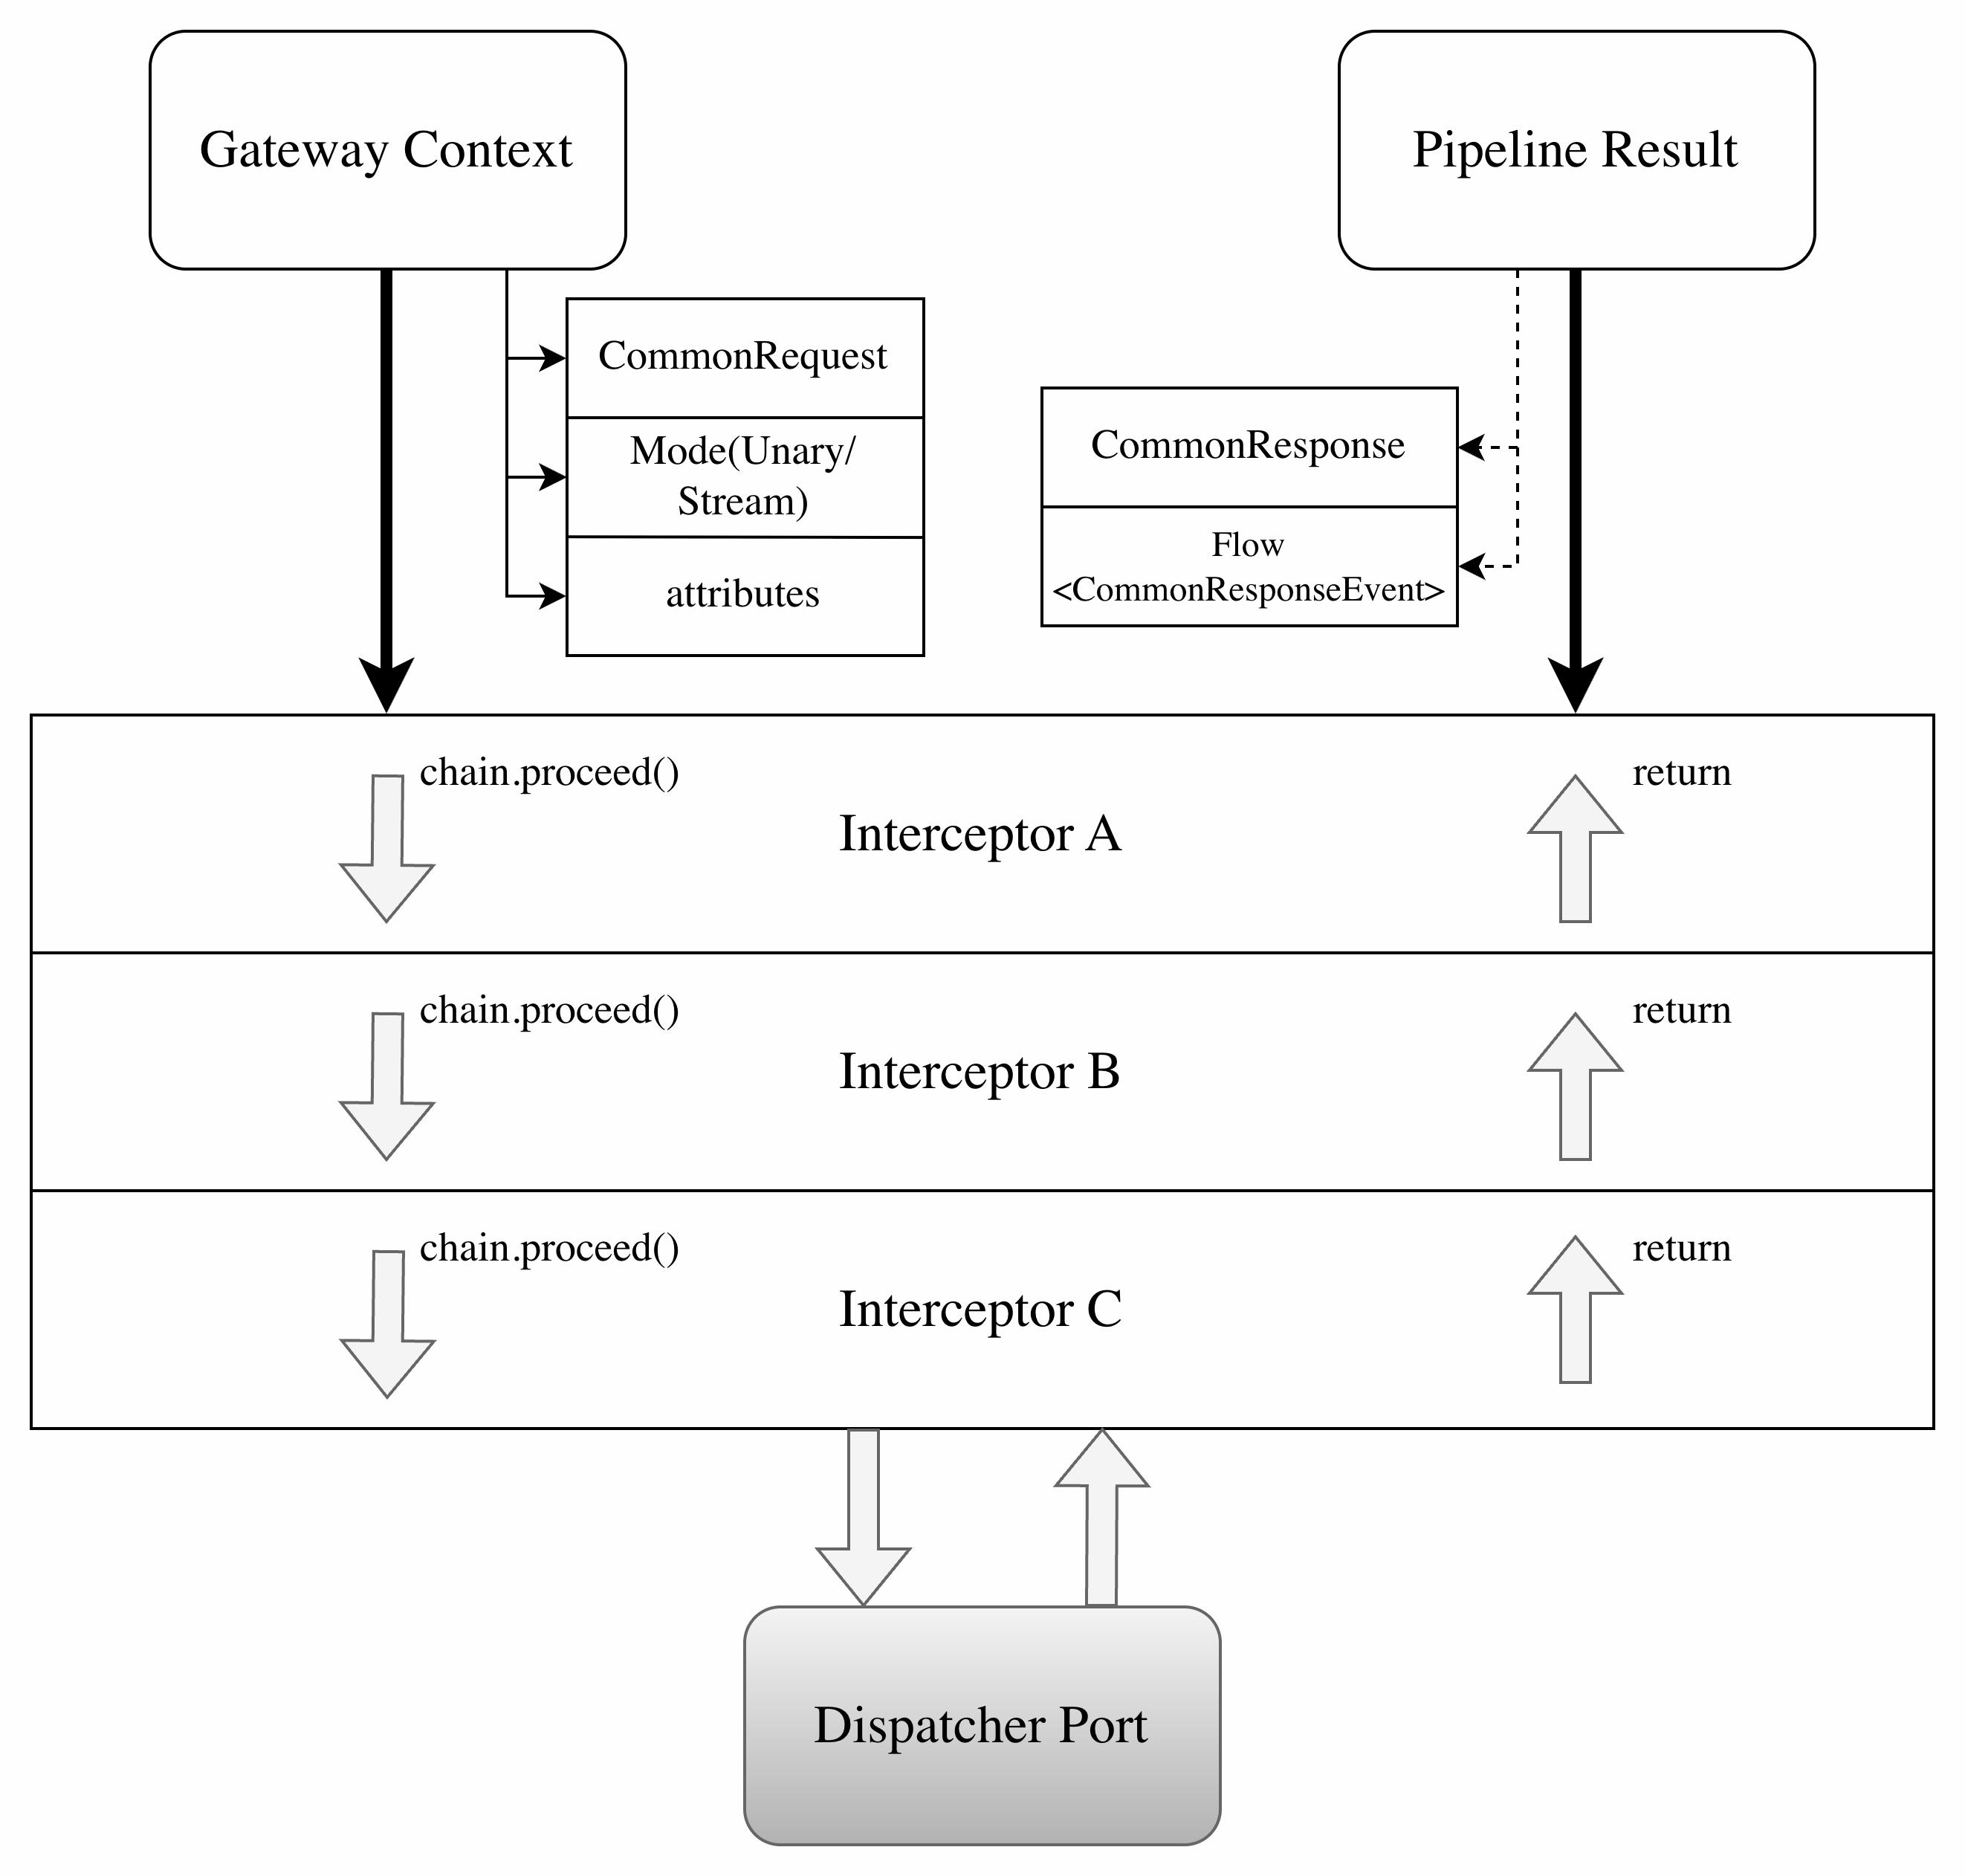
\includegraphics[width=0.9\textwidth]{../images/PipelineViewW.jpeg}
        \caption{Visão conceptual da pipeline de interceptors}
        \label{fig:pipeline}
    \end{figure}

    Esta forma de encaixe mantém a arquitetura simples. Para um caso mínimo, a Gateway pode operar com um dispatcher direto. Para um caso operacional, a pipeline permite adicionar autenticação, autorização, métricas, limites, \textit{circuit breaker}, \textit{fallback}, logging e tracing sem alterar adapters. O modelo é semelhante ao dos filtros de Servlets \cite{servlet_filterchain}: cada filtro recebe um contexto, decide se continua a cadeia e pode executar lógica antes e depois do próximo elemento. A diferença é que, no OmniAI SDK, o contexto não representa apenas um pedido HTTP; representa uma chamada de inferência já normalizada, incluindo fornecedor, modelo, modo de execução, atributos tipados e eventual fluxo de \textit{streaming}.

    A \textit{pipeline} é composta por \texttt{GatewayPipeline}, \texttt{GatewayPipelineChain}, \texttt{Interceptor} e \texttt{GatewayContext}. O \texttt{GatewayContext} transporta o pedido comum, atributos tipados e modo de execução, podendo representar chamadas síncronas ou \textit{streaming}. A cadeia executa os \textit{interceptors} por ordem e, no fim, invoca o dispatcher terminal.

    Esta abordagem também prepara o escalamento horizontal. A pipeline não exige estado global obrigatório; cada pedido transporta o seu contexto. Onde existe estado partilhável, como rate limiting ou circuit breaker, o SDK define stores substituíveis. A implementação em memória é adequada para desenvolvimento e instância única, mas pode ser trocada por Redis, base de dados ou outro backend coordenado em implantações distribuídas. Assim, várias instâncias da OmniAI Gateway podem partilhar contadores, estados de circuito e metadados operacionais sem alterar o contrato dos inbounds nem a forma como os clientes chamam a Gateway.

    \section{Arquitetura Interna dos Interceptors}
    O módulo \texttt{interceptors} inclui implementações pré-construídas para preocupações operacionais e de segurança. Todos seguem o mesmo contrato: recebem um \texttt{GatewayContext}, consultam ou acrescentam atributos à \texttt{TypedMap}, decidem se chamam \texttt{chain.proceed(context)} e podem observar ou transformar o \texttt{PipelineResult}. Esta estrutura permite colocar lógica transversal antes e depois da inferência sem acoplar essa lógica aos adapters de entrada, aos adapters de saída ou ao dispatcher.

    A ordem de execução é configurável. No target JVM, o SDK suporta a anotação \texttt{InterceptorPriority}, usada para executar primeiro interceptors com prioridade superior. No target JavaScript, onde a reflexão sobre anotações é limitada, a ordem segue a sequência definida pela DSL. Assim, autenticação e autorização podem ocorrer no início da cadeia, enquanto métricas, tracing e logging podem envolver a execução completa.

    A motivação para estes interceptors não foi apenas organizar código, mas tornar explícitas políticas que, numa Gateway de IA, afetam segurança, custo e disponibilidade. A Tabela~\ref{tab:interceptor-rationale} resume essa relação.

    \begin{table}[H]
        \centering
        \footnotesize
        \renewcommand{\arraystretch}{1.25}
        \begin{tabularx}{\textwidth}{|>{\raggedright\arraybackslash}p{3.2cm}|Y|Y|}
            \hline
            \textbf{Interceptor} & \textbf{Problema tratado} & \textbf{Motivo para estar na Gateway} \\
            \hline
            Telemetria & Falta de visibilidade sobre latência, erros, tokens e fornecedores. & A Gateway observa todas as chamadas e consegue medir comportamento transversal sem alterar clientes ou adapters. \\
            \hline
            Autenticação & Necessidade de validar quem apresenta o token antes de consumir modelos pagos. & A Gateway é o recurso protegido e deve validar tokens antes de encaminhar tráfego para fornecedores. \\
            \hline
            Autorização & Um token válido não implica permissão para todos os modelos ou operações. & A decisão por cliente, ação, fornecedor e modelo deve ser centralizada antes da inferência. \\
            \hline
            Rate limiting & Risco de abuso, picos de carga e custos inesperados. & A Gateway é o ponto natural para aplicar quotas por cliente, plano, fornecedor ou modelo. \\
            \hline
            Circuit breaker & Dependências externas podem ficar lentas ou indisponíveis. & A Gateway evita insistir em fornecedores em falha e protege o restante sistema. \\
            \hline
            Fallback & Uma falha de fornecedor não deve, quando existe alternativa, falhar imediatamente a experiência do cliente. & A Gateway conhece os outbounds disponíveis e pode tentar alternativas mantendo o contrato do cliente. \\
            \hline
        \end{tabularx}
        \caption{Justificação dos interceptors fornecidos pelo SDK}
        \label{tab:interceptor-rationale}
    \end{table}

    \subsection{Interceptor de Telemetria e Observabilidade}
    O \texttt{MetricsInterceptor} recolhe dados operacionais essenciais num sistema que intermedeia chamadas a LLMs: latência, sucesso, erro, fornecedor, modelo, cliente e consumo de tokens. Estes dados são importantes porque uma Gateway centraliza tráfego de vários clientes e fornecedores; sem telemetria, não é possível perceber custos, degradação, falhas por modelo ou impacto de políticas como \textit{fallback}.

    A implementação distingue chamadas unárias de \textit{streaming}. Em respostas progressivas, o interceptor não bloqueia a execução; usa operadores de fluxo para observar eventos e emitir métricas no encerramento do \textit{stream}. Assim mede a duração total da interação, e não apenas o tempo até ao primeiro fragmento.

    A arquitetura segue inversão de dependência através da porta \texttt{MetricsPort}. O OmniAI SDK define instrumentos comuns, como \texttt{counter}, \texttt{histogram} e \texttt{upDownCounter}, enquanto o adapter concreto no target JVM exporta para OpenTelemetry. O uso do OpenTelemetry Protocol (OTLP) foi escolhido porque o OTLP define a codificação, transporte e entrega de dados de telemetria entre fontes, coletores e backends \cite{opentelemetry_otlp}. Esta escolha evita prender o OmniAI SDK a Prometheus, Grafana, Datadog ou outro backend específico: o SDK emite telemetria num formato aberto, o Collector recebe e processa esses dados, e a infraestrutura decide para onde exportar.

    Esta decisão é especialmente importante numa Gateway de IA. O mesmo OmniAI SDK pode ser usado por uma aplicação simples em desenvolvimento, por um POC local com Prometheus/Grafana ou por uma instalação futura com outro backend de observabilidade. A OpenTelemetry apresenta-se precisamente como especificação aberta e agnóstica de fornecedor \cite{opentelemetry_what_is}; por isso, a instrumentação fica no OmniAI SDK, mas a escolha operacional do backend permanece fora do domínio.

    \begin{figure}[H]
        \centering
        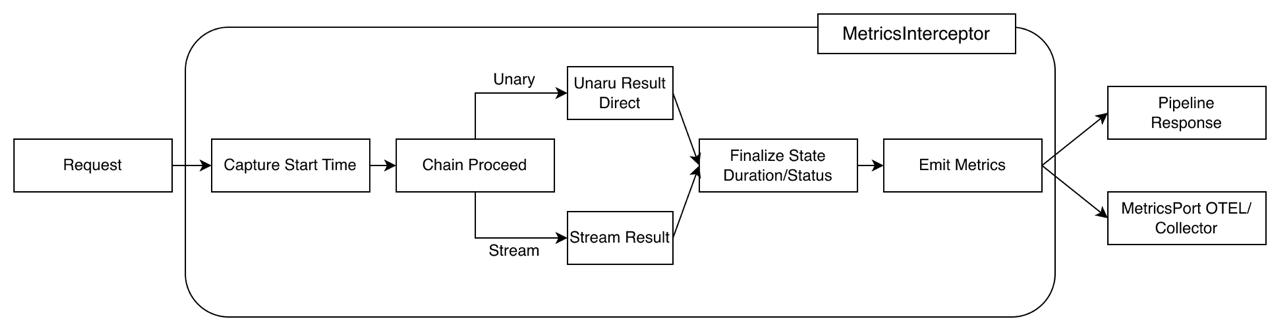
\includegraphics[width=0.9\textwidth]{../images/MetricsInterceptorArch}
        \caption{Fluxo interno de processamento e lógica de observabilidade para pedidos unários e streaming}
        \label{fig:metrics-interceptor-arch}
    \end{figure}

    Para adicionar uma métrica, a aplicação usa a DSL do \texttt{gateway-client}. O programador pode ativar a latência padrão, acrescentar atributos globais e definir métricas próprias com uma função \texttt{value}, que extrai o valor a partir do contexto e do resultado, e uma função \texttt{tags}, que acrescenta dimensões de análise.

    \begin{lstlisting}[language=kotlin, caption={Configuração de telemetria e métricas personalizadas na DSL}]
metrics {
    metricsPort = telemetryRuntime.metricsPort
    tracer = telemetryRuntime.tracer

    attributes {
        include(ClientIpMetadataKey, alias = "client.ip")
        attribute("sdk.version") { _, _ -> "1.0.0" }
    }

    defaultLatency {
        enabled = true
        name = "gateway.inference.request.duration"
    }

    customMetrics {
        counter(
            name = "gateway.llm.tokens",
            description = "Total de tokens consumidos",
            unit = "{tokens}"
        ) {
            value { _, result ->
                (result as? PipelineResult.Unary)?.response?.usage?.totalTokens
            }
        }
    }
}
    \end{lstlisting}

    Este desenho separa três responsabilidades: a definição da métrica na DSL, a recolha no interceptor e a exportação no adapter de telemetria. Também facilita testes, porque \texttt{NoOpMetricsPort} pode ser usado quando a observabilidade está desligada.

    \begin{figure}[H]
        \centering
        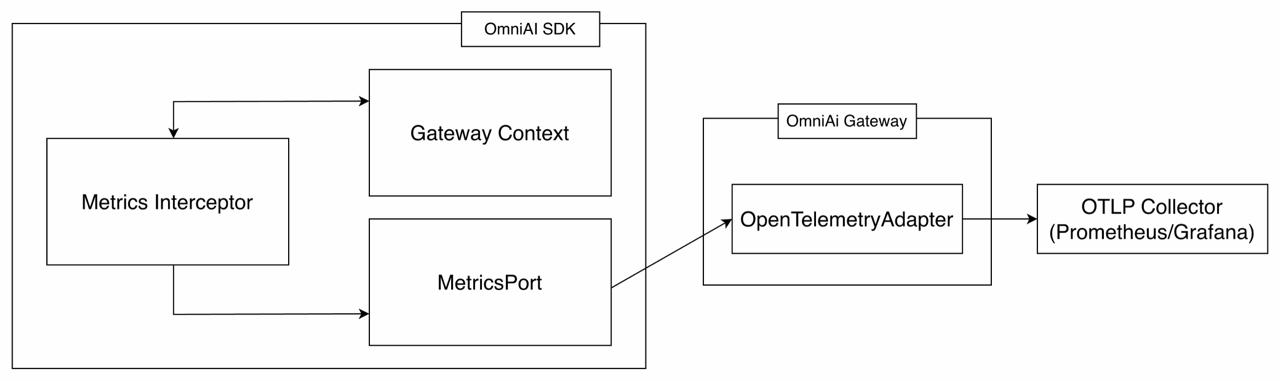
\includegraphics[width=0.9\textwidth]{../images/MetricsGateway}
        \caption{Observabilidade e métricas operacionais da OmniAI Gateway}
        \label{fig:metrics-gateway}
    \end{figure}

    \subsection{Interceptor de Autenticação}
    A autenticação é realizada pelo \texttt{AuthenticationInterceptor}. A Gateway atua como \textit{Resource Server}: recebe pedidos para recursos protegidos, extrai o \textit{access token} do cabeçalho \texttt{Authorization: Bearer <token>} e valida se esse token foi emitido por um servidor de autorização confiável \cite{rfc6749,rfc6750,oauth_resource_server}. Esta responsabilidade é essencial numa AI Gateway, porque a camada central passa a proteger acesso a modelos, custos, quotas e dados operacionais.

    A Gateway não deve atuar como \textit{Authorization Server}: não emite tokens, não gere credenciais dos clientes e não substitui Logto ou Keycloak. O seu papel é o de API protegida. Por isso, valida tokens recebidos, confirma se foram emitidos para a audiência esperada e só depois permite que o pedido avance na pipeline para os próximos interceptors Esta separação reduz responsabilidade de segurança dentro do SDK e permite integrar diferentes fornecedores de identidade sem alterar o contrato dos clientes.

    O fluxo inicia-se no adapter HTTP, que propaga o token para o domínio através de metadados. O interceptor classifica o token: se tiver três segmentos, é tratado como JWT; caso contrário, como token opaco. Esta distinção permite escolher entre validação local por assinatura e validação remota por introspeção.

    No modo \textit{OIDC Discovery} (RFC 8414), a Gateway obtém dinamicamente metadados do \textit{Authorization Server}, como \textit{issuer}, \texttt{jwks\_uri} e endpoint de introspeção \cite{rfc8414}. Todo este fluxo encontra-se ilustrado na Figura 5.4. Para JWTs, valida o \texttt{kid}, obtém a chave pública no JWKS, verifica assinatura e confirma \textit{claims} como \texttt{exp}, \texttt{nbf}, \texttt{iss} e \texttt{aud} \cite{rfc7519,rfc7517,rfc7515}. Para tokens opacos, usa introspeção OAuth2 \cite{rfc7662}.

    \begin{figure}[H]
        \centering
        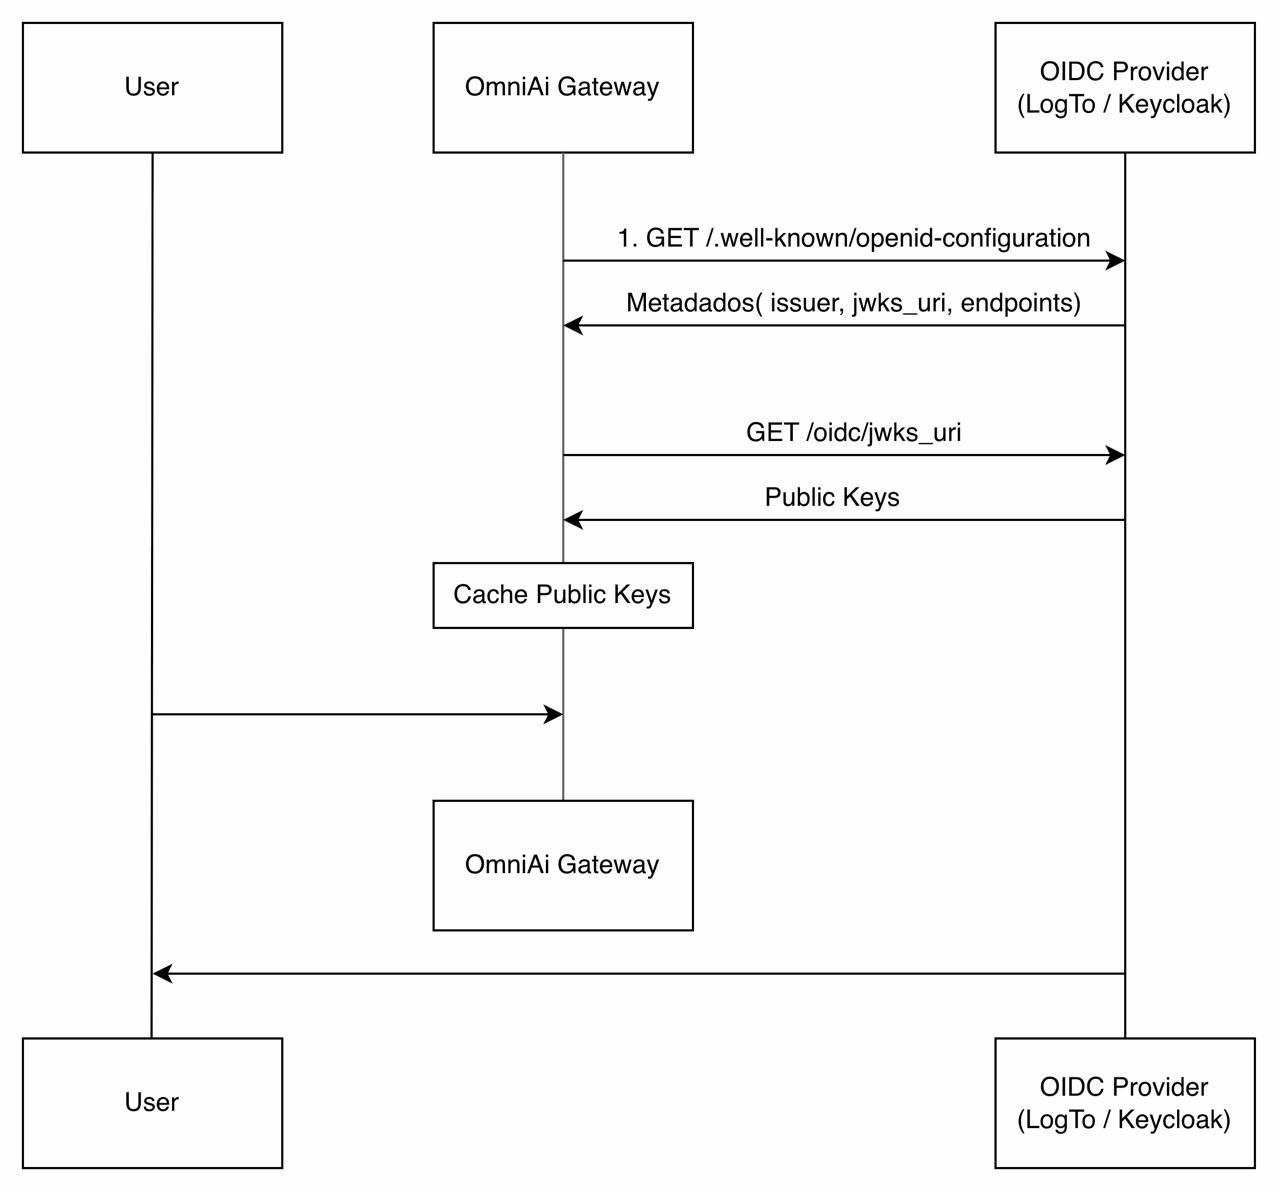
\includegraphics[width=0.9\textwidth]{../images/AutenticationFlow}
        \caption{Sequência OIDC: descoberta, JWKS e cache de chaves}
        \label{fig:oidc-sequence}
    \end{figure}

    Para reduzir latência e chamadas repetidas ao servidor de autorização, a implementação inclui \texttt{InMemoryKeyCache}, rotação de chaves em \textit{background} e \textit{cooldown} para evitar consultas excessivas quando uma chave não é encontrada. No caso de tokens opacos, o \texttt{IntrospectionCache} usa \textit{positive caching} para tokens ativos e \textit{negative caching} para tokens inválidos. Os tokens opacos são guardados em cache através de \textit{hash}, evitando manter credenciais em texto limpo em memória.

    O resultado é encapsulado em \texttt{AuthValidationResult} e guardado na \texttt{TypedMap} sob a chave \texttt{AUTH\_RESULT\_KEY}. Isto permite que autorização, métricas e logging reutilizem a identidade já validada.

    \begin{figure}[H]
        \centering
        
\includegraphics[width=\textwidth]{../images/autenticacao}
        \caption{Fluxo interno do interceptor de autenticação}
        \label{fig:auth-interceptor}
    \end{figure}

    A Gateway final usa Logto como Authorization Server local \cite{logto_docs}, executado em Docker juntamente com PostgreSQL, OpenTelemetry Collector, Prometheus e Grafana. Foram também realizados testes exploratórios com Keycloak \cite{keycloak_docs}. A escolha final do Logto no POC deveu-se à simplicidade de configuração local, suporte a aplicações Machine-to-Machine e facilidade de gerir API Resources durante a validação.

    A integração do processo de autenticação é declarada na montagem do \textit{SDK}:
    \begin{lstlisting}[language=kotlin, caption={DSL de configuração do interceptor de autenticação com OIDC Discovery}]
security {
    authentication {
        discovery {
            discoveryUrl = "https://auth.example.com/.well-known/openid-configuration"
            expectedAudience = "https://gateway.example.com/api"
            clientId = "gateway-client"
            clientSecret = "secret"
        }
    }
}
    \end{lstlisting}

    \subsection{Interceptor de Autorização}
    A autorização é separada da autenticação porque responder a ``quem é o utilizador?'' não é o mesmo que responder a ``o que este utilizador pode fazer?''. A autenticação valida identidade; a autorização decide permissões sobre uma ação e um recurso. Esta separação é importante numa Gateway multi-cliente, onde um token válido pode não ter permissão para usar todos os modelos, fornecedores ou operações. A distinção entre autenticação e autorização é também a base dos modelos modernos de identidade: a primeira prova identidade, enquanto a segunda concede permissão sobre dados ou ações protegidas \cite{microsoft_authn_authz}.

    No contexto do projeto, esta separação evita dois problemas. Primeiro, impede que a validação de token seja confundida com autorização total: um cliente autenticado pode estar limitado a um subconjunto de modelos, fornecedores ou quotas. Segundo, permite trocar a origem das decisões de autorização sem alterar a autenticação. Embora numa fase inicial a decisão possa operar de forma local e simples, o sistema está desenhado para que, numa iteração futura, essa mesma decisão possa ser assegurada por um PDP externo, tal como o AuthZen ou o OPA.

    No OmniAI SDK, a autorização é centralizada no \texttt{PolicyEnforcerInterceptor}. O componente atua como \textit{Policy Enforcement Point} (PEP): interceta o pedido, constrói um \texttt{AuthorizationInput} e delega a decisão a um \textit{Policy Decision Point} (PDP) através da porta \texttt{PolicyDecisionPointPort}.Podemos ver todo este fluxo na figura 5.6.

    \begin{figure}[H]
        \centering
        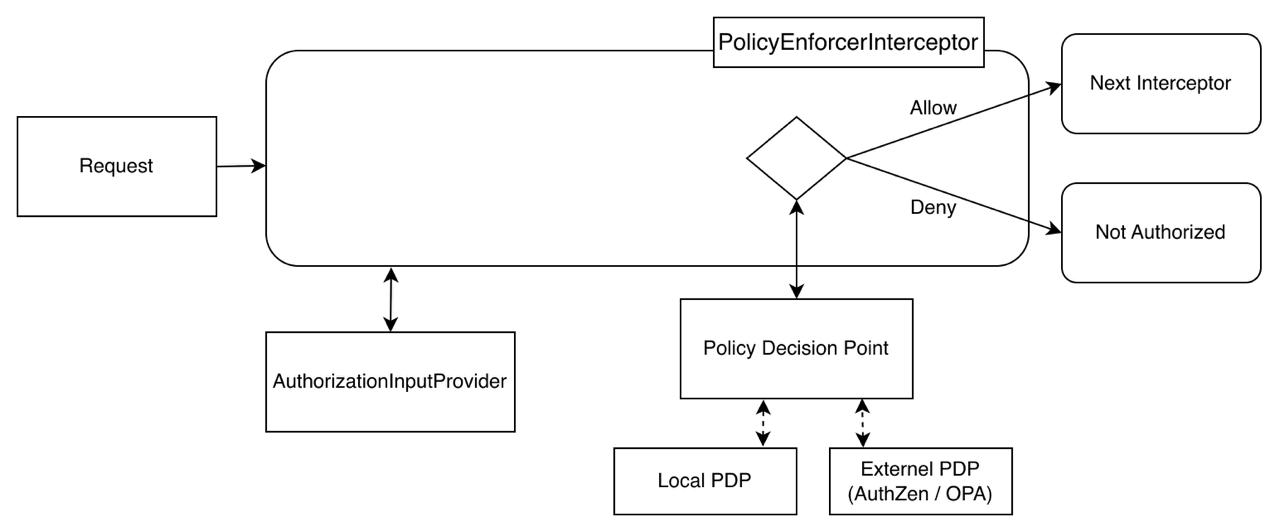
\includegraphics[width=0.9\textwidth]{../images/Authorization}
        \caption{Arquitetura do interceptor de autorização: separação entre PEP e PDP}
        \label{fig:authorization-architecture}
    \end{figure}

    O \texttt{AuthorizationInput} segue o padrão \textbf{Subject-Action-Resource (SAR)}. O \textbf{Subject} representa o utilizador ou aplicação, incluindo identificador, roles e atributos vindos do token. A \textbf{Action} representa a operação, como \texttt{chat\_completion}. O \textbf{Resource} identifica o alvo, como fornecedor ou modelo. O \textbf{Context} acrescenta atributos ambientais, como IP, tempo ou metadados do pedido. A porta do PDP permite integrar motores diferentes, incluindo políticas internas, AuthZen, OPA ou outro serviço externo. Se a decisão for \textit{Deny}, a pipeline é interrompida antes de qualquer chamada ao fornecedor \cite{authorization_pips}.

    A configuração de autorização permite estender o avaliador por omissão:
    \begin{lstlisting}[language=kotlin, caption={DSL de configuração do interceptor de autorização}]
security {
    authorization {
        pdp = customPolicyDecisionPoint
        inputProvider = DefaultAuthorizationInputProvider
    }
}
    \end{lstlisting}

    \subsection{Interceptor de Rate Limiting}
    O \texttt{RateLimitInterceptor} aplica limites de utilização antes da chamada ao fornecedor. Numa AI Gateway, este mecanismo tem dois objetivos principais: proteger o sistema contra abuso ou tráfego excessivo e controlar custos associados a chamadas de inferência. A limitação de taxa é uma estratégia comum para impor um teto de ações repetidas num intervalo temporal, reduzindo abuso de APIs, força bruta e carga excessiva \cite{cloudflare_rate_limiting}.

    A importância deste interceptor é maior do que numa API tradicional, porque cada pedido pode representar custo financeiro direto, consumo de quotas externas e ocupação prolongada de ligações em \textit{streaming}. Sem rate limiting, um cliente mal configurado, uma automação em ciclo ou um utilizador abusivo pode saturar a Gateway, esgotar quotas nos fornecedores e degradar o serviço para clientes legítimos. O interceptor permite aplicar justiça operacional: cada cliente, plano, modelo ou fornecedor pode ter limites próprios.

    A lógica é orientada por políticas. Cada \texttt{RateLimitPolicy} extrai dados do \texttt{GatewayContext} e devolve \texttt{RateLimitTarget}. Um target contém uma chave, como cliente/modelo/plano, e uma \texttt{RateLimitDefinition}, composta por limite, tipo e janela temporal. Isto permite políticas diferentes por cliente, plano, modelo ou fornecedor.

    O store atual em memória usa buckets protegidos por \texttt{Mutex}. Quando um pedido chega, o interceptor tenta consumir uma unidade em todos os buckets aplicáveis. Se todos permitirem consumo, a cadeia continua. Se algum limite estiver esgotado, devolve \texttt{TooManyRequestsError} com \texttt{retryAfter}. Esta resposta permite que clientes bem comportados reduzam ritmo em vez de insistirem. Para desenvolvimento e instância única, este modelo é suficiente; em escalamento horizontal, o contrato \texttt{RateLimitStore} permite substituir a implementação por Redis ou outro backend partilhado. Essa substituição é necessária quando várias instâncias da Gateway devem partilhar a mesma visão de quota.

    A configuração deste mecanismo recorre ao seguinte bloco:
    \begin{lstlisting}[language=kotlin, caption={DSL de configuração do interceptor de rate limiting}]
interceptors {
    rateLimiting {
        store = InMemoryRateLimitStore()
        addPolicy(rateLimitPolicy)
    }
}
    \end{lstlisting}

    \subsection{Interceptor de Circuit Breaker}
    O \texttt{CircuitBreakerInterceptor} protege a Gateway contra chamadas repetidas a um outbound em falha. O padrão de \textit{circuit breaker} é usado para lidar com falhas em serviços remotos, evitando insistir numa dependência que está indisponível e dando tempo para recuperação \cite{microsoft_circuit_breaker,itau_circuit_breaker,treinaweb_circuit_breaker}. Numa Gateway de IA, esta proteção é especialmente útil porque fornecedores externos podem falhar por indisponibilidade, timeouts, quotas ou erros 5xx.

    A alternativa simples seria repetir pedidos até obter sucesso. Essa abordagem é perigosa quando o fornecedor está realmente indisponível: as tentativas acumulam latência, ocupam threads ou corrotinas, aumentam custos e podem agravar a falha no serviço externo. O circuit breaker foi criado para evitar esse comportamento. Quando a falha ultrapassa um limiar, o circuito abre e a Gateway passa a falhar rapidamente aquele destino, libertando recursos e permitindo que mecanismos como fallback escolham outro outbound.

    Para cada combinação de fornecedor/modelo, o interceptor identifica o \texttt{outbound.key} e consulta o \texttt{CircuitBreakerStore}. Se o circuito estiver \texttt{OPEN}, o pedido falha rapidamente com \texttt{ApiDownError} e o outbound é acrescentado ao conjunto de outbounds negados no contexto. Esta falha rápida reduz latência, evita consumo de recursos e dá ao \textit{fallback} informação para não tentar novamente o mesmo destino.

    Quando a chamada prossegue, o interceptor observa o resultado. Erros incrementam o contador de falhas; ao atingir \texttt{failureThreshold}, o circuito passa para \texttt{OPEN}. Após um período de recuperação, o estado \texttt{HALF\_OPEN} permite testar um número limitado de pedidos antes de voltar ao estado \texttt{CLOSED}, evitando inundar um fornecedor que ainda está a recuperar \cite{microsoft_circuit_breaker}. A configuração inclui \texttt{failureThreshold}, \texttt{resetTimeoutMs} e \texttt{halfOpenTestRequests}. A implementação atual cobre a abertura e fecho básico do circuito; a evolução temporal mais completa do estado \texttt{HALF\_OPEN} é uma melhoria natural.

    \begin{lstlisting}[language=kotlin, caption={DSL de configuração do interceptor de circuit breaker}]
interceptors {
    circuitBreaker {
        store = InMemoryCircuitBreakerStore()
        config = CircuitBreakerConfig(
            failureThreshold = 5,
            resetTimeoutMs = 10000L,
            halfOpenTestRequests = 2
        )
    }
}
    \end{lstlisting}

    \subsection{Interceptor de Fallback}
    O \texttt{FallbackInterceptor} permite tentar alternativas quando a chamada principal falha. Em sistemas de IA, \textit{fallback} ao nível de modelo ou fornecedor é relevante porque falhas nas APIs de inferência fornecidas pelas LLM's são um cenário frequente em produção: rate limits, indisponibilidade, quotas, timeouts ou modelos descontinuados podem impedir a resposta do fornecedor principal \cite{ai_fallback_tombas,portkey_fallback}. Um gateway é o ponto certo para esta política, porque conhece os outbounds configurados e consegue trocar de destino sem exigir alterações no cliente.

    A decisão de colocar fallback na Gateway, e não nos clientes, reduz duplicação e melhora controlo operacional. Se cada aplicação cliente implementasse a sua própria lógica de fallback, seria necessário repetir regras de prioridade, tratamento de erros, mapeamento de contratos e métricas em vários pontos. Ao centralizar a política, o SDK consegue manter o mesmo contrato de entrada e decidir internamente que fornecedor ou modelo alternativo deve ser tentado. Isto é particularmente útil quando o cliente usa um contrato compatível com Anthropic ou OpenAI, mas a Gateway pode executar a chamada noutro provider configurado.

    A implementação atual usa a lista de outbounds disponíveis. Primeiro tenta o outbound correspondente ao fornecedor e modelo pedidos; se falhar, acrescenta esse outbound ao conjunto de negados e tenta alternativas. Para cada tentativa, cria um novo \texttt{GatewayContext} com os mesmos atributos, mas com \texttt{provider} e \texttt{model} atualizados para o outbound alternativo.

    A integração com o circuit breaker é feita através do conjunto partilhado de outbounds negados. Assim, se um circuito estiver aberto, o fallback evita esse destino e tenta outro modelo ou fornecedor. Este desenho permite construir políticas de resiliência como ``tentar Gemini, depois OpenAI-compatible via Groq, depois Anthropic'', mantendo a lógica de tentativa fora dos adapters. Também permite distinguir degradação controlada de erro total: a resposta pode chegar por um modelo alternativo, enquanto métricas e tracing registam que ocorreu fallback.

    A evolução futura poderá acrescentar prioridades configuráveis, condições por código de erro, orçamentos de tentativa e métricas específicas de fallback. Estas regras são importantes porque nem todo erro justifica fallback: erros de autenticação ou autorização devem falhar imediatamente, enquanto timeouts, 429 e 5xx podem justificar uma alternativa.

    A sua ativação é extremamente simples, não requerendo configuração intrincada:
    \begin{lstlisting}[language=kotlin, caption={DSL de configuração do interceptor de fallback}]
interceptors {
    fallback()
}
    \end{lstlisting}

    \subsection{Interceptor de Logging e Tracing}
    O \texttt{RequestLoggingInterceptor} regista fornecedor, modelo, sucesso, erro e conclusão de streams através da abstração \texttt{GatewayLogger}. No target JVM pode ser ligado a SLF4J; no target JavaScript pode usar consola ou outra integração. O objetivo é garantir visibilidade mínima mesmo quando a telemetria completa não está ativa.

    O logging foi mantido separado das métricas porque responde a perguntas diferentes. Métricas mostram tendências agregadas, como latência média ou número de erros; logs ajudam a explicar um pedido concreto. Numa Gateway de IA, esta distinção também tem impacto de privacidade: o objetivo é registar metadados operacionais, e não despejar prompts, respostas completas ou tokens sensíveis nos logs.

    O \texttt{TracingInterceptor} envolve o pedido num \textit{span} chamado \texttt{gateway.request.process}. Quando combinado com OpenTelemetry, este span permite correlacionar latência, erros, chamadas externas e métricas agregadas. Em cenários de fallback ou circuit breaker, tracing é particularmente útil porque permite observar o percurso real do pedido e distinguir falhas do fornecedor, decisões da Gateway e erros de cliente. Também permite perceber se uma resposta lenta resulta do fornecedor principal, de uma tentativa alternativa, de validação de token ou de uma política interna.

    A instalação processa-se em dois blocos da DSL, um explícito e outro decorrente da configuração de métricas:
    \begin{lstlisting}[language=kotlin, caption={Instalação dos interceptors de logging e tracing}]
interceptors {
    // Instalacao manual do Logging Interceptor
    use(RequestLoggingInterceptor(logger))
    
    // O TracingInterceptor e instalado automaticamente ao fornecer o tracer as metricas
    metrics {
        tracer = telemetryRuntime.tracer
    }
}
    \end{lstlisting}

    \section{MCP Broker e Ferramentas Externas}

    O MCP Broker foi introduzido como consequência do estudo do MCP e do \textit{tool calling}. O objetivo é separar a gestão de ferramentas externas da lógica específica das APIs de inferência. Em vez de cada adapter conhecer diretamente as ferramentas disponíveis e a forma como são executadas, o broker fornece uma camada intermédia para representar ferramentas, recursos e \textit{prompts} de forma uniforme.

    O módulo \texttt{mcp-broker} depende da biblioteca \texttt{io.modelcontextprotocol:kotlin-sdk}. A implementação atual inclui modelos para ferramentas, recursos e \textit{prompts}, geração de esquemas JSON, configuração de transportes \texttt{stdio}, SSE e WebSocket, e mapeamento entre o domínio do projeto e tipos do SDK MCP. A classe \texttt{McpTool} descreve uma ferramenta por nome, descrição, serializer e função \texttt{execute}; \texttt{McpServerBuilder} permite registar ferramentas, recursos e \textit{prompts} de forma declarativa.

    A Figura~\ref{fig:tool-calling} representa o ciclo geral de \textit{tool calling}. Primeiro, o cliente envia um pedido com ferramentas disponíveis. Em seguida, o modelo pode pedir uma chamada estruturada com nome e argumentos. A aplicação executa ou encaminha a ferramenta, devolve o resultado ao modelo e recebe a resposta final. O MCP Broker foi desenhado para suportar esta separação no futuro, permitindo que ferramentas sejam registadas e disponibilizadas sem acoplar cada adapter de inferência ao conjunto concreto de ferramentas.

    \begin{figure}[H]
        \centering
        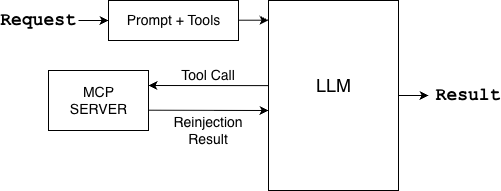
\includegraphics[width=0.45\textwidth]{../images/ToolCallingCycle}
        \caption{Representação do ciclo de \textit{tool calling} e interação com ferramentas externas}
        \label{fig:tool-calling}
    \end{figure}

    No estado atual, o módulo estabelece sobretudo as abstrações, os modelos e o mapeamento necessários para essa evolução. A execução completa de ferramentas via MCP Broker, o carregamento por YAML e a integração no POC OmniAI Gateway permanecem como trabalho futuro. Esta delimitação é importante: o POC valida contratos HTTP, autenticação, telemetria e consumo do SDK, mas ainda não demonstra invocação real via MCP Broker.

    \section{Distribuição Multiplataforma}

    Um dos objetivos do OmniAI SDK é permitir que a lógica principal da Gateway seja reutilizada em diferentes ambientes de execução. O Kotlin Multiplatform permite separar código comum de implementações específicas: o domínio, contratos, portas, adapters principais, DSL e parte dos interceptors vivem em source sets comuns; detalhes como cliente HTTP, reflexão de prioridades, servidor Ktor e integrações de plataforma ficam em source sets específicos.

    No target JVM, o OmniAI-SDK pode ser utilizado por aplicações Kotlin ou Java. Este é o target mais consolidado no estado atual do projeto e é o usado pelo POC OmniAI Gateway. A implementação JVM inclui Ktor HTTP client, integração com servidor Ktor, autenticação com descoberta OIDC, telemetria e execução real de outbounds. A distribuição futura via Maven permitirá que uma aplicação adicione o SDK como dependência versionada, sem depender de \textit{composite build}.

    No target JavaScript/Node.js, o projeto prepara uma API consumível a partir do ecossistema Node.js e TypeScript. A fachada \texttt{@JsExport} encapsula a configuração em tipos exportáveis e evita expor diretamente estruturas Kotlin que não são adequadas à fronteira JS. Esta camada é uma base para consumo via NPM, mas ainda não tem paridade total com a JVM.

    A nuance principal da distribuição multiplataforma é que nem tudo deve ser comum. O domínio e os contratos devem permanecer partilhados; transporte HTTP, servidor, observabilidade e segurança podem ter implementações diferentes por plataforma. Esta divisão evita duplicação sem forçar uma abstração demasiado rígida. A linha de evolução prevista é consolidar a API pública do OmniAI-SDK, estabilizar versionamento semântico, automatizar publicação Maven/NPM por CD e documentar exemplos mínimos de consumo para JVM e Node.js.


    \chapter{Provas de Conceito (PoCs) e Validação}

    \section{Validação do POC OmniAI Gateway}
    A validação principal foi realizada com a aplicação \texttt{OmniAiGateway}, um POC que consome o OmniAI SDK através do \textit{composite build}. Esta aplicação carrega o ficheiro \texttt{application.conf}, resolve variáveis de ambiente, instancia o \texttt{KtorHttpTransportClient}, configura outbounds, ativa segurança e telemetria, monta o runtime do SDK e expõe endpoints HTTP compatíveis com OpenAI, Anthropic e Gemini.

    O comportamento validado não deve ser descrito como roteamento inteligente. A implementação atual realiza despacho configurado: o pedido contém fornecedor e modelo, e o dispatcher padrão escolhe o outbound que corresponde a essa combinação. Este desenho já permite demonstrar o desacoplamento entre cliente e fornecedor, mas políticas mais avançadas, como seleção por custo, qualidade, latência ou plano do cliente, permanecem como trabalho futuro. O trabalho de \textit{fallback} e \textit{circuit breaker} fornece a base técnica para esse tipo de evolução, mas o POC não afirma executar roteamento semântico ou otimizado.

    \begin{figure}[H]
        \centering
        \begin{tikzpicture}[
        % node distance: vertical, horizontal
            node distance=0.8cm and 1.5cm,
        % Estilo uniforme para as caixas de cliente e fornecedores
            box/.style={rectangle, draw, rounded corners, align=center, text width=4.0cm, minimum height=1.4cm, inner sep=5pt, thick},
        % Estilo para a gateway (maior e com preenchimento)
            gateway/.style={rectangle, draw, rounded corners, align=center, text width=4.5cm, minimum height=2.5cm, inner sep=6pt, fill=gray!15, thick},
            arrow/.style={-Latex, thick}
        ]
            % --- COLUNA ESQUERDA ---
            \node[box] (rest) {REST Client};
            \node[box, below=0.8cm of rest] (claude) {Claude Code\\ \texttt{ANTHROPIC\_BASE\_URL}};
            \node[box, below=0.8cm of claude] (node) {SDK Anthropic\\ Node.js};

            % --- GATEWAY CENTRAL ---
            \node[gateway, right=of claude] (gateway) {\textbf{OmniAI Gateway POC}};

            % --- COLUNA DIREITA ---
            % Ajuste de yshift para espaçamento vertical no lado direito
            \node[box, right=of gateway, yshift=1.2cm] (providers) {Fornecedor configurado\\ Gemini, OpenAI\\ Anthropic};
            \node[box, right=of gateway, yshift=-1.2cm] (obs) {Prometheus + Grafana\\ via OpenTelemetry Collector};

            % --- LIGAÇÕES ---
            \draw[arrow] (rest.east) -- (gateway.west);
            \draw[arrow] (claude.east) -- (gateway.west);
            \draw[arrow] (node.east) -- (gateway.west);

            \draw[arrow] (gateway.east) -- (providers.west);
            \draw[arrow] (gateway.east) -- (obs.west);
        \end{tikzpicture}
        \caption{Cenários de validação do POC OmniAI Gateway}
        \label{fig:poc-validation}
    \end{figure}

    \section{Validação com REST Client}
    O ficheiro \texttt{gateway-requests.http} foi usado para validar manualmente os endpoints expostos pela Gateway. Este ficheiro contém pedidos para \texttt{/v1/chat/completions}, \texttt{/v1/messages} e \texttt{/v1beta/models/\{model\}:generateContent}, cobrindo respostas unárias, \textit{streaming}, geração com parâmetros e integração com token Bearer.

    Este cenário foi importante por duas razões. Primeiro, permitiu validar a forma exata dos contratos HTTP recebidos pelo POC sem depender de uma aplicação externa complexa. Segundo, permitiu testar rapidamente o fluxo completo: token emitido pelo Logto, pedido autenticado, tradução inbound, despacho para outbound, chamada ao fornecedor configurado e resposta no contrato esperado pelo cliente.

    \section{Validação de Segurança com Logto}
    A camada de segurança foi validada com Logto como Authorization Server local. O ambiente Docker inclui Logto, PostgreSQL, OpenTelemetry Collector, Prometheus e Grafana. A configuração do POC usa OIDC Discovery para obter metadados do servidor de autorização e validar tokens com audiência configurada para o recurso da API.

    Durante o desenvolvimento foram realizados testes exploratórios com Keycloak, mas a configuração final mudou para Logto por reduzir a complexidade operacional do POC. O Logto facilitou a criação de API Resources, aplicações Machine-to-Machine e fluxos OIDC adequados à validação da Gateway como Resource Server.

    O fluxo também foi validado com \texttt{run\_claude.py}. Este script abre o browser para autenticação no Logto, usa PKCE, troca o código por um token e inicia o Claude Code com \texttt{ANTHROPIC\_BASE\_URL} a apontar para a OmniAI Gateway. O cabeçalho \texttt{Authorization} é injetado através de \texttt{ANTHROPIC\_CUSTOM\_HEADERS}, permitindo testar um cliente real compatível com Anthropic a passar pela Gateway.

    \section{Validação de Observabilidade}
    A observabilidade foi validada com OpenTelemetry Collector, Prometheus e Grafana. O POC ativa métricas na DSL do SDK, incluindo latência padrão, contagem de tokens e contagem de erros. Também acrescenta atributos como IP do cliente, versão do SDK, audiência e dados derivados do resultado de autenticação, como \texttt{sub}, \texttt{email} ou \texttt{preferred\_username} quando disponíveis.

    O objetivo desta validação foi confirmar que a Gateway consegue produzir telemetria em tempo real enquanto processa pedidos reais. A utilização de Prometheus e Grafana permitiu observar métricas operacionais da aplicação e confirmar que a instrumentação está separada da lógica de inferência, sendo configurada através da DSL e exportada por adapters próprios.

    \section{Validação com Aplicações Cliente}
    Foram estudados e testados cenários com clientes que permitem alterar o endpoint da API. No caso do Claude Code, a variável \texttt{ANTHROPIC\_BASE\_URL} permite redirecionar pedidos para a Gateway. \\
    Foi criado um teste com o sdk oficial da anthropic em \texttt{node-tests/anthropicSDKTest.js}, configurado com \texttt{baseURL} local e chave fictícia, para validar que um cliente existente consegue falar com a OmniAI Gateway quando esta expõe um contrato compatível.

    Também foram estudadas aplicações como OpenCode, LibreChat e Dify, por permitirem configurar endpoints compatíveis com fornecedores existentes. Estes estudos demonstram o valor arquitetural da Gateway: quando o cliente já segue um contrato conhecido, a introdução da OmniAI Gateway pode ser feita por configuração de endpoint, sem alterar a lógica principal da aplicação cliente.

    \section{Limites da Validação}
    A validação realizada confirma o consumo do SDK pelo POC, a exposição HTTP com Ktor, a integração com Logto, o uso de Prometheus/Grafana e a compatibilidade com clientes reais ou semi-reais. No entanto, existem limites importantes. O POC ainda não demonstra invocação de ferramentas via MCP Broker, nem políticas avançadas de roteamento por custo, latência ou qualidade. Estes pontos dependem de trabalho futuro sobre o módulo \texttt{mcp-broker}, sobre políticas de dispatcher e sobre stores distribuídos para cenários multi-instância.


    \chapter{Conclusões e Trabalho Futuro}

    \section{Conclusão}

    No momento em que o desenvolvimento deste projeto teve início, a adoção de componentes de infraestrutura dedicados a intermediar aplicações e APIs de inferência era ainda uma prática pouco comum. A falta de arquiteturas e de produtos consolidados fazia com que a maioria das aplicações integrasse diretamente as APIs dos fornecedores, o que limitava a escalabilidade, a segurança e a gestão de chaves de API, de utilizadores e de outras questões fundamentais, como a imposição de limites, a implementação de mecanismos de resiliência e a recolha de métricas.

    Contudo, à medida que este projeto foi sendo desenvolvido, começaram a surgir cada vez mais soluções de intermediação de inferência (\textit{AI Gateways}), reforçando ainda mais a importância do problema que procurámos resolver. Esta evolução veio demonstrar que o projeto desenvolvido é relevante, não apenas pelos desafios técnicos que apresenta, mas também pela crescente valorização deste tipo de soluções no mercado.

    A principal diferença introduzida por este projeto é o facto de ter sido desenvolvido um \textit{Software Development Kit} (\textbf{SDK}) e não apenas uma aplicação final. Foi desenvolvida uma biblioteca completamente abstrata e customizável, recorrendo a \textbf{Kotlin Multiplatform}. Esta abordagem torna-se particularmente interessante porque não disponibiliza apenas um produto pronto a utilizar, com regras de negócio específicas, mas sim uma base reutilizável sobre a qual qualquer utilizador pode construir a solução que melhor se adapta às suas necessidades. Apesar de esta decisão ter aumentado a complexidade do projeto, acreditamos que foi também um dos aspetos que mais o diferencia das soluções existentes.

    O uso de \textbf{Kotlin Multiplatform} permite instanciar uma \textit{OmniAiGateway} em dois \textit{targets} distintos, JVM e Node.js. Embora tenham existido dificuldades associadas ao desenvolvimento de uma biblioteca em \textbf{Kotlin Multiplatform}, estas foram ultrapassadas, permitindo disponibilizar uma solução em ambas as plataformas. Este aspeto aumenta ainda mais a flexibilidade do projeto, facilitando a sua adoção em sistemas já existentes, quer na JVM quer em Node.js.

    Ao longo deste trabalho foi possível concretizar um \textbf{SDK} reutilizável e abstrato, incorporando as funcionalidades apresentadas ao longo deste relatório. Foi possível normalizar as APIs de inferência da \textbf{OpenAI} \cite{openai_api}, \textbf{Anthropic} \cite{anthropic_api} e \textbf{Gemini}, suportando igualmente rotas de entrada compatíveis com as mesmas e permitindo encaminhar os pedidos para APIs de inferência compatíveis com esses formatos. Isto permite que aplicações de IA generativa já existentes, desenvolvidas para qualquer um destes fornecedores, consigam utilizar o nosso sistema praticamente sem alterações, mantendo compatibilidade com os formatos esperados enquanto passam a beneficiar de funcionalidades adicionais.

    Sendo este um projeto bastante abstrato e configuravel, é possível configurar uma \textit{gateway} com diferentes níveis de complexidade. Pode ser utilizada apenas como uma peça de infraestrutura mais simples que encaminha pedidos para o mesmo fornecedor de inferência do pedido, acrescentando funcionalidades como métricas, \textit{rate limiting}, autenticação ou autorização. Por outro lado, pode também suportar cenários muito mais avançados, como roteamento inteligente entre modelos e fornecedores com base em latência ou algoritmos semânticos, mecanismos de \textit{caching} de respostas de inferência ou mesmo ao nível do MCP. Ao optar por esta abordagem, o nosso objetivo foi precisamente permitir que quem utiliza o \textbf{SDK} tenha liberdade para implementar funcionalidades que vão além daquelas que nós próprios desenvolvemos.

    Naturalmente, este projeto apresentou também vários desafios. Um dos principais foi lidar com as diferenças existentes entre os vários fornecedores de inferência. Apesar de, à primeira vista, as APIs parecerem semelhantes, são extremamente extensas, contêm inúmeros conceitos proprietários e nem sempre possuem documentação suficientemente explícita. Construir um domínio comum sobre estas APIs foi, para nós, um dos maiores feitos alcançados neste projeto e um resultado do qual nos orgulhamos bastante.

    Outro desafio importante foi garantir a evolução e manutenção da normalização criada. As APIs de inferência encontram-se em constante evolução e, durante o desenvolvimento deste projeto, surgiram diversas atualizações que obrigaram à adaptação da nossa implementação. Além disso, normalizar não apenas pedidos e respostas, mas também eventos de \textit{streaming}, exigiu um esforço adicional devido às diferenças existentes entre fornecedores, tornando esta componente particularmente desafiante.

    De forma a demonstrar a utilização prática do \textbf{SDK}, foi realizada a instanciação de uma \textit{OmniAi Gateway} e a sua integração com o \textbf{Claude Code}. Conseguir utilizar um agente amplamente utilizado e, através da nossa \textit{gateway}, comunicar com modelos da Google, nomeadamente o \textbf{Gemini}, foi um resultado que consideramos particularmente marcante. Durante o desenvolvimento deste trabalho não encontrámos nenhuma solução que permitisse este tipo de interoperabilidade da mesma forma, pelo que acreditamos que este projeto apresenta um caráter bastante inovador.

    A integração da camada de inferência com o \textbf{MCP Broker} foi também um elemento fundamental do projeto. Para além de nos permitir aprofundar o conhecimento sobre o protocolo \textbf{MCP}, possibilitou igualmente a implementação de um sistema interessante e totalmente integrado com a restante arquitetura.

    Consideramos que, no final, a implementação do projeto apresenta uma qualidade técnica muito elevada e cumpre os objetivos inicialmente definidos. Ao longo do desenvolvimento tivemos oportunidade de aprofundar conhecimentos em arquiteturas como \textit{Ports and Adapters}, na construção de um sistema que atua como \textit{Resource Server}, implementando os RFCs apropriados, na utilização de padrões de autorização como \textit{Policy Enforcement Point} e \textit{Policy Decision Point}, bem como na adoção do \textbf{OpenTelemetry} e na construção de \textit{dashboards} no \textbf{Grafana}. O sistema continua em evolução e existem ainda muitas funcionalidades que gostaríamos de implementar. Tratando-se de um \textbf{SDK}, existe sempre espaço para acrescentar novas capacidades. Para além dos desafios técnicos, uma das maiores dificuldades foi também definir um âmbito que fosse simultaneamente ambicioso e realista. No final, acreditamos que este projeto resultou numa solução sólida e tecnicamente diferenciadora, contribuindo também de forma significativa para a evolução das nossas competências enquanto engenheiros.



    \section{Melhorias Futuras e Escalabilidade}
    Como trabalho futuro, existem várias linhas de evolução. A primeira é consolidar a distribuição pública do \textbf{SDK} via \textbf{Maven} e \textbf{NPM}, garantindo documentação de instalação, versionamento semântico e exemplos de consumo. A segunda é completar a paridade entre \textit{targets} \textbf{JVM} e \textbf{JavaScript}, sobretudo na montagem de \textit{runtime} e transporte \textbf{HTTP}.

    Outra melhoria importante é aprofundar o \textbf{MCP Broker}, incluindo carregamento efetivo de ferramentas via \textbf{YAML}, execução completa dos \textit{handlers} \textbf{MCP} e suporte robusto a \textbf{SSE} e \textbf{WebSocket}. Também será relevante melhorar as políticas de roteamento, permitindo decisões com base em custo, latência, disponibilidade, qualidade do modelo, plano do cliente e limites de utilização.

    Por fim, a camada de segurança pode evoluir para políticas de autorização mais expressivas, integração com PDPs externos, introspeção real de \textit{tokens} opacos e mapeamento mais fino entre \textit{claims}, planos e quotas. A nível de infraestrutura, perspetiva-se a adoção de um cofre de segredos (\textit{Key Vault}) \cite{ref_keyVault}  para o armazenamento e gestão centralizada e segura das \textit{API Keys} de inferência. 
    
    Na parte da testabilidade também será fundamental alargar a validação do sistema através da implementação de testes de integração mais abrangentes e de (\textit{stress testing}), garantindo a estabilidade em casos de cenários de uso intensivo. 
    
    Estas melhorias permitiriam aproximar a \textbf{OmniAI Gateway} de uma solução robusta e pronta para ambientes \textit{multi-tenant} \cite{ref_MultiTenant} e de produção.


% ================= APÊNDICES =================
    \appendix

    \chapter{Detalhe dos Campos do Modelo de Domínio}
\label{apendice:dominio}

\section{Pedido}

\begin{table}[H]
    \centering
    \scriptsize % Fonte ligeiramente mais pequena para evitar overflow no rodapé
    \setlength{\tabcolsep}{3.5pt} % Menos espaço nas laterais para aproveitar melhor a largura
    \renewcommand{\arraystretch}{1.15}
    \begin{tabularx}{\textwidth}{|>{\raggedright\arraybackslash}p{2.9cm}|>{\raggedright\arraybackslash}p{2.6cm}|>{\raggedright\arraybackslash}p{2.6cm}|>{\raggedright\arraybackslash}X|}
    \hline
    \textbf{Elemento} & \textbf{Campo} & \textbf{Tipo} & \textbf{Descrição} \\ \hline

    CommonRequest & provider & Provider & Fornecedor alvo da chamada. \\ \hline
    CommonRequest & model & String & Identificador do modelo a utilizar. \\ \hline
    CommonRequest & messages & List<Common\-RequestMessage> & Histórico de mensagens enviado ao modelo. \\ \hline
    CommonRequest & systemPrompt & SystemPrompt? & Prompt de sistema global (opcional). \\ \hline
    CommonRequest & config & Common\-GenerationConfig? & Parâmetros de geração (opcional). \\ \hline
    CommonRequest & tools & List<CommonTool> & Ferramentas disponíveis para chamadas de função. \\ \hline
    CommonRequest & toolChoice & ToolChoice? & Política de seleção de ferramentas. \\ \hline
    CommonRequest & jsonResponse & Boolean & Indica se a resposta deve ser forçada a JSON. \\ \hline
    CommonRequest & providerOptions & TypedMap & Opções específicas do fornecedor. \\ \hline

    CommonRequest\-Message & role & CommonRole & Papel da mensagem (SYSTEM, USER, ASSISTANT, TOOL). \\ \hline
    CommonRequest\-Message & content & List<Request\-ContentPart> & Conteúdo segmentado da mensagem. \\ \hline

    SystemPrompt & text & String & Conteúdo do prompt de sistema. \\ \hline

    Common\-GenerationConfig & temperature & Double? & Grau de aleatoriedade da geração. \\ \hline
    Common\-GenerationConfig & maxTokens & Int? & Limite máximo de \textit{tokens} de saída. \\ \hline
    Common\-GenerationConfig & topP & Double? & Probabilidade cumulativa. \\ \hline
    Common\-GenerationConfig & stopSequences & List<String>? & Sequências que interrompem a geração. \\ \hline

    CommonTool & name & String & Nome da ferramenta. \\ \hline
    CommonTool & description & String & Descrição funcional da ferramenta. \\ \hline
    CommonTool & parametersSchema & JsonObjectMap & Esquema JSON dos parâmetros. \\ \hline

    ToolChoice & Auto / None / Required / Specific & -- & Estratégia de uso de ferramentas (auto, nenhuma, obrigatório ou lista específica). \\ \hline
    ToolChoiceAuto & -- & -- & Subtipo sem campos (seleção automática). \\ \hline
    ToolChoiceNone & -- & -- & Subtipo sem campos (sem ferramentas). \\ \hline
    ToolChoiceRequired & -- & -- & Subtipo sem campos (uso obrigatório). \\ \hline
    ToolChoiceSpecific & toolNames & List<String> & Lista de ferramentas permitidas. \\ \hline

    Provider & value & String & Identificador textual do fornecedor. \\ \hline
    TypedMap & data & Map<String, Any?> & Mapa genérico de opções específicas do fornecedor. \\ \hline

    RequestContentPart & TextPart & text: String & Conteúdo textual. \\ \hline
    RequestContentPart & JsonPart & json: JsonValue & Conteúdo JSON estruturado. \\ \hline
    RequestContentPart & ToolCallPart & toolCallId,\newline functionName,\newline argumentsJson & Chamada a ferramenta com argumentos. \\ \hline
    RequestContentPart & ToolResultPart & toolCallId,\newline content & Resultado de execução de ferramenta. \\ \hline

    \end{tabularx}
    \caption{Parâmetros do domínio de \texttt{CommonRequest}.}
    \label{tab:request-parametros}
\end{table}

\section{Resposta e Eventos}


 \begin{table}[H]
    \centering
    \scriptsize
    \setlength{\tabcolsep}{4pt}
    \renewcommand{\arraystretch}{1.2}
    \begin{tabularx}{\textwidth}{|>{\raggedright\arraybackslash}p{3.4cm}|>{\raggedright\arraybackslash}p{2.2cm}|>{\raggedright\arraybackslash}p{3.8cm}|>{\raggedright\arraybackslash}X|}
        \hline
        \textbf{Elemento} & \textbf{Campo} & \textbf{Tipo} & \textbf{Descrição} \\ \hline

        CommonResponse & \textit{provider} & Provider & Fornecedor que produziu a resposta. \\ \hline
        CommonResponse & id & String & Identificador do pedido/execução. \\ \hline
        CommonResponse & model & String & Identificador do modelo utilizado. \\ \hline
        CommonResponse & choices & List<CommonChoice> & Lista de escolhas geradas. \\ \hline
        CommonResponse & usage & CommonUsage? & Contabilização de \textit{tokens} (opcional). \\ \hline
        CommonResponse & providerOptions & Map<String, Any?> & Metadados específicos do fornecedor. \\ \hline

        CommonChoice & index & Int & Índice da escolha. \\ \hline
        CommonChoice & message & CommonResponseMessage & Mensagem com papel e conteúdo. \\ \hline
        CommonChoice & finishReason & FinishReason? & Razão de término da escolha (opcional). \\ \hline

        CommonResponseMessage & role & CommonRole & Papel da mensagem. \\ \hline
        CommonResponseMessage & content & List<ResponseContentPart> & Conteúdo segmentado da resposta. \\ \hline

        CommonUsage & inputTokens & Int? & Tokens de entrada. \\ \hline
        CommonUsage & outputTokens & Int? & Tokens de saída. \\ \hline
        CommonUsage & totalTokens & Int? & Total de \textit{tokens}. \\ \hline

        % Correção solicitada: O enum foi para a coluna 'Tipo' e formatado com quebras limpas
        FinishReason & -- & STOP / LENGTH / \newline TOOL\_CALL / \newline CONTENT\_FILTER / \newline OTHER & Motivo de conclusão da geração. \\ \hline

        ResponseContentPart & TextPart & text: String & Segmento textual. \\ \hline
        ResponseContentPart & JsonPart & json: JsonValue & Segmento JSON estruturado. \\ \hline
        ResponseContentPart & ToolCallPart & toolCallId, \newline functionName, \newline argumentsJson & Chamada a ferramenta. \\ \hline
        ResponseContentPart & RefusalPart & reason: String & Recusa do modelo com justificação. \\ \hline

    \end{tabularx}
    \caption{Parâmetros do domínio de \textit{Response} (CommonResponse).}
    \label{tab:response-parametros}
\end{table}



\begin{table}[H]
    \centering
    \scriptsize
    \setlength{\tabcolsep}{4pt}
    \renewcommand{\arraystretch}{1.2}
    \begin{tabularx}{\textwidth}{|>{\raggedright\arraybackslash}p{3.5cm}|>{\raggedright\arraybackslash}p{2.5cm}|>{\raggedright\arraybackslash}p{2.0cm}|>{\raggedright\arraybackslash}X|}
        \hline
        \textbf{Elemento} & \textbf{Campo} & \textbf{Tipo} & \textbf{Descrição} \\ \hline

        CommonResponse\newline Event & \textit{provider} & Provider & Fornecedor associado ao evento. \\ \hline
        CommonResponse\newline Event & id & String & Identificador do pedido/execução. \\ \hline
        CommonResponse\newline Event & model & Model & Modelo utilizado no evento. \\ \hline
        CommonResponse\newline Event & sequence & Long & Ordem do evento no \textit{stream}. \\ \hline
        CommonResponse\newline Event & \textit{provider}\newline EventType & String? & Tipo bruto do evento do fornecedor (opcional). \\ \hline

        ResponseStarted & -- & -- & Início do \textit{streaming} da resposta. \\ \hline

        ChoiceStarted & choiceIndex & Int & Índice da escolha iniciada. \\ \hline
        ChoiceStarted & role & CommonRole? & Papel associado à escolha (opcional). \\ \hline

        TextDeltaEvent & choiceIndex & Int & Índice da escolha que recebe o delta. \\ \hline
        TextDeltaEvent & text & String & Fragmento incremental de texto. \\ \hline

        ToolCall\newline StartedEvent & choiceIndex & Int & Índice da escolha. \\ \hline
        ToolCall\newline StartedEvent & toolCallIndex & Int & Índice da chamada a ferramenta. \\ \hline
        ToolCall\newline StartedEvent & toolCallId & String & Identificador da chamada a ferramenta. \\ \hline
        ToolCall\newline StartedEvent & functionName & String & Nome da função invocada. \\ \hline

        ToolCallArguments\newline DeltaEvent & choiceIndex & Int & Índice da escolha. \\ \hline
        ToolCallArguments\newline DeltaEvent & toolCallIndex & Int & Índice da chamada a ferramenta. \\ \hline
        ToolCallArguments\newline DeltaEvent & arguments\newline Fragment & String & Fragmento incremental de argumentos. \\ \hline

        ChoiceFinished & choiceIndex & Int & Índice da escolha terminada. \\ \hline
        ChoiceFinished & finishReason & FinishReason? & Razão de término (opcional). \\ \hline

        UsageReported & usage & CommonUsage & Contabilização de \textit{tokens} reportada. \\ \hline

        ResponseCompleted & -- & -- & Conclusão do \textit{streaming} da resposta. \\ \hline

        ResponseErrored & message & String & Mensagem de erro. \\ \hline
        ResponseErrored & retryable & Boolean & Indica se o erro é recuperável. \\ \hline

    \end{tabularx}
    \caption{Parâmetros do domínio de \textit{Response} (CommonResponseEvent).}
    \label{tab:response-events-parametros}
\end{table}


    % ================= APÊNDICE: JSONs das APIs de Inferência =================
\chapter{Exemplos JSON das APIs de Inferência}
\label{apx:json-apis}

Este apêndice reúne os exemplos completos dos corpos JSON utilizados durante o estudo das APIs de inferência. Os exemplos incluem pedidos e respostas de geração de texto, chamadas de ferramentas (\textit{tool calling}), \textit{streaming} e configuração de raciocínio (\textit{thinking}), permitindo ao leitor consultar as estruturas integrais que foram analisadas e comparadas no Capítulo~2.

% ---------------------------------------------------------------
\section{Pedidos (\textit{Requests})}
\label{apx:json-requests}
% ---------------------------------------------------------------

\subsection{\textbf{OpenAI} (formato compatível)}

\begin{lstlisting}[language=json, caption={Pedido básico à API da \textbf{OpenAI} (geração com \textit{system prompt})}]
{
  "model": "llama3.2:1b",
  "messages": [
    {
      "role": "system",
      "content": "Es um assistente local a correr em Docker."
    },
    {
      "role": "user",
      "content": "Ola! Estas a funcionar?"
    }
  ],
  "temperature": 0.7
}
\end{lstlisting}

\begin{lstlisting}[language=json, caption={Pedido à API da \textbf{OpenAI} com ferramentas (\textit{tool calling})}]
{
  "model": "llama3.2:1b",
  "messages": [
    {
      "role": "user",
      "content": "Como esta o preco das acoes da Apple (AAPL)?"
    }
  ],
  "tools": [
    {
      "type": "function",
      "function": {
        "name": "get_stock_price",
        "description": "Obtem o preco atual de uma acao",
        "parameters": {
          "type": "object",
          "properties": {
            "symbol": {
              "type": "string",
              "description": "O ticker da empresa, ex: AAPL"
            }
          },
          "required": ["symbol"]
        }
      }
    }
  ],
  "tool_choice": "auto"
}
\end{lstlisting}

\begin{lstlisting}[language=json, caption={Pedido à API da \textbf{OpenAI} com todos os parâmetros de geração}]
{
  "model": "llama-3.3-70b-versatile",
  "messages": [
    {
      "role": "system",
      "content": "Es um assistente tecnico que responde apenas em topicos."
    },
    {
      "role": "user",
      "content": "Explica a diferenca entre CPU e GPU."
    }
  ],
  "temperature": 0.5,
  "max_tokens": 1024,
  "top_p": 1,
  "stream": false,
  "stop": ["FIM", "TERMINAR"],
  "presence_penalty": 0.0,
  "frequency_penalty": 0.0,
  "seed": 42,
  "user": "utilizador_123",
  "response_format": { "type": "text" },
  "logit_bias": null
}
\end{lstlisting}

\begin{lstlisting}[language=json, caption={Pedido \textit{stream} à API da \textbf{OpenAI}}]
{
  "model": "llama3.2:1b",
  "messages": [
    {
      "role": "user",
      "content": "O que e Kubernetes?"
    }
  ],
  "stream": true
}
\end{lstlisting}

\subsection{\textbf{Anthropic}}

\begin{lstlisting}[language=json, caption={Pedido básico à API da \textbf{Anthropic} (geração com \textit{system prompt})}]
{
  "model": "claude-3-5-haiku-20241022",
  "max_tokens": 1024,
  "system": "You are a cat. Your name is Neko.",
  "messages": [
    {
      "role": "user",
      "content": "Hello there"
    }
  ]
}
\end{lstlisting}

\begin{lstlisting}[language=json, caption={Pedido à API da \textbf{Anthropic} com ferramentas (\textit{tool calling})}]
{
  "model": "claude-3-5-haiku-20241022",
  "max_tokens": 1024,
  "messages": [
    {
      "role": "user",
      "content": "What is the weather like in Lisbon?"
    }
  ],
  "tools": [
    {
      "name": "get_weather",
      "description": "Get the current weather in a given location",
      "input_schema": {
        "type": "object",
        "properties": {
          "location": {
            "type": "string",
            "description": "The city and country, e.g. Lisbon, Portugal"
          }
        },
        "required": ["location"]
      }
    }
  ]
}
\end{lstlisting}

\begin{lstlisting}[language=json, caption={Pedido à API da \textbf{Anthropic} com parâmetros de amostragem}]
{
  "model": "claude-3-5-haiku-20241022",
  "max_tokens": 1024,
  "temperature": 1.0,
  "top_p": 0.8,
  "top_k": 10,
  "stop_sequences": ["Title"],
  "messages": [
    {
      "role": "user",
      "content": "Explain how AI works"
    }
  ]
}
\end{lstlisting}

\begin{lstlisting}[language=json, caption={Pedido à API da \textbf{Anthropic} com raciocínio (\textit{thinking})}]
{
  "model": "claude-3-7-sonnet-20250219",
  "max_tokens": 4096,
  "thinking": {
    "type": "enabled",
    "budget_tokens": 2048
  },
  "messages": [
    {
      "role": "user",
      "content": "How does AI work?"
    }
  ]
}
\end{lstlisting}

\begin{lstlisting}[language=json, caption={Pedido \textit{stream} à API da \textbf{Anthropic}}]
{
  "model": "claude-3-5-haiku-20241022",
  "max_tokens": 200,
  "messages": [
    {
      "role": "user",
      "content": "Explain AI."
    }
  ],
  "stream": true
}
\end{lstlisting}

\subsection{\textbf{Google Gemini}}

\begin{lstlisting}[language=json, caption={Pedido básico à API do \textbf{Gemini} (geração com \textit{system instruction})}]
{
  "system_instruction": {
    "parts": [
      { "text": "You are a cat. Your name is Neko." }
    ]
  },
  "contents": [
    {
      "parts": [
        { "text": "Hello there" }
      ]
    }
  ]
}
\end{lstlisting}

\begin{lstlisting}[language=json, caption={Pedido à API do \textbf{Gemini} com ferramentas (\textit{tool calling})}]
{
  "contents": [
    {
      "role": "user",
      "parts": [
        {
          "text": "Schedule a meeting with Bob for tomorrow."
        }
      ]
    }
  ],
  "tools": [
    {
      "functionDeclarations": [
        {
          "name": "schedule_meeting",
          "description": "Schedules a meeting with attendees.",
          "parameters": {
            "type": "object",
            "properties": {
              "attendees": {
                "type": "array",
                "items": { "type": "string" }
              },
              "date": { "type": "string" },
              "time": { "type": "string" },
              "topic": { "type": "string" }
            },
            "required": ["attendees", "date", "time", "topic"]
          }
        }
      ]
    }
  ]
}
\end{lstlisting}

\begin{lstlisting}[language=json, caption={Pedido à API do \textbf{Gemini} com configuração de geração e \textit{thinking}}]
{
  "contents": [
    {
      "parts": [
        { "text": "Explain how AI works" }
      ]
    }
  ],
  "generationConfig": {
    "stopSequences": ["Title"],
    "temperature": 1.0,
    "topP": 0.8,
    "topK": 10,
    "thinkingConfig": {
      "include_thoughts": true,
      "thinkingLevel": "low"
    }
  }
}
\end{lstlisting}

\begin{lstlisting}[language=json, caption={Pedido \textit{stream} à API do \textbf{Gemini} (URI com \texttt{?alt=sse})}]
{
  "contents": [
    {
      "parts": [
        { "text": "Explain how AI works" }
      ]
    }
  ]
}
\end{lstlisting}

% ---------------------------------------------------------------
\section{Respostas (\textit{Responses})}
\label{apx:json-responses}
% ---------------------------------------------------------------

\subsection{\textbf{OpenAI} (formato compatível)}

\begin{lstlisting}[language=json, caption={Resposta completa da API da \textbf{OpenAI} (geração básica)}]
{
  "id": "chatcmpl-31",
  "object": "chat.completion",
  "created": 1773531116,
  "model": "llama3.2:1b",
  "system_fingerprint": "fp_ollama",
  "choices": [
    {
      "index": 0,
      "message": {
        "role": "assistant",
        "content": "Desculpe, mas posso tentar ajuda-lo!"
      },
      "finish_reason": "stop"
    }
  ],
  "usage": {
    "prompt_tokens": 46,
    "completion_tokens": 40,
    "total_tokens": 86
  }
}
\end{lstlisting}

\begin{lstlisting}[language=json, caption={Resposta da API da \textbf{OpenAI} (chamada de ferramenta)}]
{
  "id": "chatcmpl-53",
  "object": "chat.completion",
  "created": 1773531604,
  "model": "llama3.2:1b",
  "system_fingerprint": "fp_ollama",
  "choices": [
    {
      "index": 0,
      "message": {
        "role": "assistant",
        "content": "",
        "tool_calls": [
          {
            "id": "call_9fasug2c",
            "index": 0,
            "type": "function",
            "function": {
              "name": "get_stock_price",
              "arguments": "{\"symbol\":\"AAPL\"}"
            }
          }
        ]
      },
      "finish_reason": "tool_calls"
    }
  ],
  "usage": {
    "prompt_tokens": 171,
    "completion_tokens": 19,
    "total_tokens": 190
  }
}
\end{lstlisting}

\begin{lstlisting}[language=json, caption={Resposta \textit{stream} da \textbf{OpenAI} (eventos \textbf{SSE})}]
data: {"id":"chatcmpl-308","object":"chat.completion.chunk",
  "created":1773532270,"model":"llama3.2:1b",
  "choices":[{"index":0,
    "delta":{"role":"assistant","content":"K"},
    "finish_reason":null}]}

data: {"id":"chatcmpl-308","object":"chat.completion.chunk",
  "created":1773532270,"model":"llama3.2:1b",
  "choices":[{"index":0,
    "delta":{"content":"ubernetes "},
    "finish_reason":null}]}

data: {"id":"chatcmpl-308","object":"chat.completion.chunk",
  "created":1773532272,"model":"llama3.2:1b",
  "choices":[{"index":0,
    "delta":{},
    "finish_reason":"stop"}]}

data: [DONE]
\end{lstlisting}

\subsection{\textbf{Anthropic}}

\begin{lstlisting}[language=json, caption={Resposta completa da API da \textbf{Anthropic} (geração básica)}]
{
  "id": "msg_01Xf...",
  "type": "message",
  "role": "assistant",
  "model": "claude-3-5-haiku-20241022",
  "content": [
    {
      "type": "text",
      "text": "Artificial intelligence (AI) is a complex field..."
    }
  ],
  "stop_reason": "end_turn",
  "usage": {
    "input_tokens": 14,
    "output_tokens": 350
  }
}
\end{lstlisting}

\begin{lstlisting}[language=json, caption={Resposta da API da \textbf{Anthropic} (chamada de ferramenta)}]
{
  "id": "msg_01Cd...",
  "type": "message",
  "role": "assistant",
  "content": [
    {
      "type": "text",
      "text": "I can help you check the weather in Lisbon."
    },
    {
      "type": "tool_use",
      "id": "toolu_01A02B03C",
      "name": "get_weather",
      "input": { "location": "Lisbon, Portugal" }
    }
  ],
  "stop_reason": "tool_use"
}
\end{lstlisting}

\begin{lstlisting}[language=json, caption={Resposta da API da \textbf{Anthropic} (raciocínio \textit{thinking})}]
{
  "id": "msg_01xyz...",
  "type": "message",
  "role": "assistant",
  "model": "claude-3-7-sonnet-20250219",
  "content": [
    {
      "type": "thinking",
      "thinking": "Here I need to explain how AI works...",
      "signature": "zxcvbnm1234567890..."
    },
    {
      "type": "text",
      "text": "Artificial Intelligence (AI) works fundamentally by..."
    }
  ],
  "stop_reason": "end_turn",
  "stop_sequence": null,
  "usage": {
    "input_tokens": 13,
    "output_tokens": 850
  }
}
\end{lstlisting}

\begin{lstlisting}[language=json, caption={Resposta \textit{stream} da \textbf{Anthropic} (eventos \textbf{SSE})}]
event: message_start
data: {"type": "message_start",
  "message": {"id": "msg_d6d...", "role": "assistant",
    "model": "claude-3-5-haiku-20241022"}}

event: content_block_start
data: {"type": "content_block_start", "index": 0,
  "content_block": {"type": "text"}}

event: content_block_delta
data: {"type": "content_block_delta", "index": 0,
  "delta": {"type": "text_delta", "text": "Artificial"}}

event: content_block_delta
data: {"type": "content_block_delta", "index": 0,
  "delta": {"type": "text_delta", "text": " intelligence"}}

event: content_block_stop
data: {"type": "content_block_stop", "index": 0}

event: message_stop
data: {"type": "message_stop"}
\end{lstlisting}

\begin{lstlisting}[language=json, caption={Devolução de resultado de ferramenta na API da \textbf{Anthropic}}]
{
  "role": "user",
  "content": [
    {
      "type": "tool_result",
      "tool_use_id": "toolu_01A02B03C",
      "content": "The weather is 18C and sunny."
    }
  ]
}
\end{lstlisting}

\subsection{\textbf{Google Gemini}}

\begin{lstlisting}[language=json, caption={Resposta completa da API do \textbf{Gemini} (geração básica)}]
{
  "candidates": [
    {
      "content": {
        "parts": [
          {
            "text": "At its simplest level, AI works by...",
            "thoughtSignature": "..."
          }
        ],
        "role": "model"
      },
      "finishReason": "STOP",
      "index": 0
    }
  ],
  "usageMetadata": {
    "promptTokenCount": 5,
    "candidatesTokenCount": 969,
    "totalTokenCount": 1480,
    "promptTokensDetails": [
      { "modality": "TEXT", "tokenCount": 5 }
    ],
    "thoughtsTokenCount": 506
  },
  "modelVersion": "gemini-3-flash-preview",
  "responseId": "feKyafqAEJ_VvdIP5s7TSA"
}
\end{lstlisting}

\begin{lstlisting}[language=json, caption={Resposta da API do \textbf{Gemini} (chamada de ferramenta)}]
{
  "candidates": [
    {
      "content": {
        "parts": [
          {
            "functionCall": {
              "name": "schedule_meeting",
              "args": {
                "time": "10:00",
                "date": "2025-03-27",
                "attendees": ["Bob", "Alice"],
                "topic": "Q3 planning"
              },
              "id": "fcaog9xf"
            },
            "thoughtSignature": "..."
          }
        ],
        "role": "model"
      },
      "finishReason": "STOP",
      "index": 0,
      "finishMessage": "Model generated function call(s)."
    }
  ],
  "usageMetadata": {
    "promptTokenCount": 203,
    "candidatesTokenCount": 54,
    "totalTokenCount": 423,
    "promptTokensDetails": [
      { "modality": "TEXT", "tokenCount": 203 }
    ],
    "thoughtsTokenCount": 166
  },
  "modelVersion": "gemini-3-flash-preview",
  "responseId": "AueyadTFGvKlvdIPrv74QA"
}
\end{lstlisting}

\begin{lstlisting}[language=json, caption={Resposta \textit{stream} do \textbf{Gemini} (padrão \textbf{SSE})}]
data: {"candidates": [
  {"content": {"parts": [
    {"text": "AI works by "}
  ], "role": "model"}, "index": 0}
], "usageMetadata": {
  "promptTokenCount": 4,
  "candidatesTokenCount": 25,
  "totalTokenCount": 608,
  "thoughtsTokenCount": 579
}, "modelVersion": "gemini-3-flash-preview"}

data: {"candidates": [
  {"content": {"parts": [
    {"text": "processing data."}
  ], "role": "model"}, "index": 0}
], "usageMetadata": {
  "promptTokenCount": 4,
  "candidatesTokenCount": 51,
  "totalTokenCount": 634,
  "thoughtsTokenCount": 579
}, "modelVersion": "gemini-3-flash-preview"}

data: {"candidates": [
  {"content": {"parts": [
    {"text": "", "thoughtSignature": "..."}
  ], "role": "model"},
  "finishReason": "STOP", "index": 0}
], "usageMetadata": {
  "promptTokenCount": 4,
  "candidatesTokenCount": 853,
  "totalTokenCount": 1436,
  "thoughtsTokenCount": 579
}, "modelVersion": "gemini-3-flash-preview"}
\end{lstlisting}

    \chapter{Mapeamentos Fornecedores}
\label{apendice:mapeamentos-fornecedores}

    \section{Tradutores de Entrada (Inbound)}
    \subsection{\textbf{OpenAI} Inbound Translator}

A implementação \texttt{OpenAiInboundTranslator} adapta os contratos compatíveis com a API da \textbf{OpenAI} para o domínio comum.
    
\begin{table}[H]
    \centering
    \footnotesize
    \renewcommand{\arraystretch}{1.25}
    \begin{tabularx}{\textwidth}{|>{\ttfamily\raggedright\arraybackslash}p{4cm}|Y|}
        \hline
        \textbf{Contrato Inbound (OpenAI)} & \textbf{Mapeamento para CommonRequest} \\
        \hline
        temperature, maxTokens, topP &
        Integrados na \texttt{CommonGenerationConfig}. O campo \texttt{model} é mapeado diretamente para o nível superior do \texttt{CommonRequest}. \\
        \hline
        stop &
        É convertido para uma \texttt{List<String>}, distinguindo automaticamente entre valores únicos (\texttt{Single}) e múltiplos (\texttt{Multiple}). \\
        \hline
        messages[].role &
        Convertido para os papéis do domínio comum: \texttt{SYSTEM}, \texttt{ASSISTANT}, \texttt{TOOL} e \texttt{USER}. Valores não reconhecidos são tratados como \texttt{USER}. \\
        \hline
        messages[].content \& toolCalls &
        O conteúdo textual não vazio origina instâncias de \texttt{TextPart}. As chamadas de ferramentas são convertidas em \texttt{ToolCallPart(toolCallId, functionName)}, com os argumentos encapsulados num mapa sob a chave \texttt{"raw"}; se o identificador vier omisso, é gerado no formato \texttt{"openai-tool-call-\$index"}. Quando o papel é \texttt{TOOL} e existem \texttt{toolCallId} e conteúdo, é gerado um \texttt{ToolResultPart}, convertendo o conteúdo textual para valor JSON. \\
        \hline
        tools[].function &
        Convertido para \texttt{CommonTool(name, description, parametersSchema)}, extraindo as propriedades definidas no schema da ferramenta. Se a descrição estiver ausente, é usado o nome da função; se os parâmetros estiverem ausentes, o schema fica vazio. \\
        \hline
        toolChoice &
        Converte os valores \texttt{auto}, \texttt{none} e \texttt{required} para os respetivos tipos do domínio comum (\texttt{ToolChoice.Auto}, \texttt{ToolChoice.None} e \texttt{ToolChoice.Required}), podendo também representar a seleção explícita de uma função específica. \\
        \hline
        responseFormat &
        Verifica se o tipo corresponde a \texttt{"json\_object"} ou \texttt{"json\_schema"}, ativando a opção \texttt{jsonResponse}. \\
        \hline
        \textit{stream}, frequencyPenalty, presencePenalty, n, seed, user, logitBias, logProbs, topLogProbs, responseFormat &
        Armazenados na \texttt{TypedMap} (\texttt{providerOptions}) do \texttt{CommonRequest}, preservando opções específicas do fornecedor que não possuem representação no domínio comum. \\
        \hline
    \end{tabularx}
    \caption{Mapeamento Inbound: \textbf{OpenAI} Request para o Domínio Comum}
    \label{tab:openai-inbound-mapping}
\end{table}


No sentido inverso, a tradução da resposta converte os objetos do domínio comum para a estrutura nativa da API da \textbf{OpenAI}.

\begin{table}[H]
    \centering
    \footnotesize
    \renewcommand{\arraystretch}{1.25}
    \begin{tabularx}{\textwidth}{|>{\ttfamily\raggedright\arraybackslash}p{4cm}|Y|}
        \hline
        \textbf{Domínio Comum} & \textbf{Mapeamento para Contrato Resposta (OpenAI)} \\
        \hline
        id \& created &
        Utiliza o \texttt{id} nativo ou gera um identificador no formato \texttt{chatcmpl-UUID}. O instante temporal é recuperado das \texttt{providerOptions} ou gerado pelo \texttt{Clock.System}; o \texttt{systemFingerprint}, quando existe, também é recuperado das \texttt{providerOptions}. \\
        \hline
        choices[].message.role &
        Convertido de \texttt{CommonRole} para os papéis nativos da \textbf{OpenAI}: \texttt{system}, \texttt{user}, \texttt{assistant} ou \texttt{tool}. \\
        \hline
        choices[].message.content &
        O conteúdo é obtido através de \texttt{firstRenderableContentOrNull()}, juntando os \texttt{TextPart} com quebras de linha. Se não existir texto, recorre ao primeiro \texttt{RefusalPart} ou à representação textual do primeiro \texttt{JsonPart}. \\
        \hline
        choices[].message
        .toolCalls &
        Um \texttt{ToolCallPart} é convertido para um \texttt{OpenAiToolCallOutput}, formatando os \texttt{argumentsJson} numa única representação textual. \\
        \hline
        choices[].finishReason &
        Converte \texttt{STOP} para \texttt{stop}, \texttt{LENGTH} para \texttt{length}, \texttt{TOOL\_CALL} para \texttt{tool\_calls} e \texttt{CONTENT\_FILTER} para \texttt{content\_filter}. Valores \texttt{OTHER} ou nulos não são emitidos. \\
        \hline
        usage &
        Mapeia \texttt{inputTokens}, \texttt{outputTokens} e \texttt{totalTokens} para \texttt{promptTokens}, \texttt{completionTokens} e \texttt{totalTokens}, respetivamente. \\
        \hline
    \end{tabularx}
    \caption{Mapeamento Inbound: Domínio para \textbf{OpenAI} Response Unária}
\end{table}


Para respostas em \textit{streaming}, os eventos internos do domínio são convertidos para os \textit{chunks} \textbf{SSE} utilizados pela \textbf{OpenAI}.

\begin{table}[H]
    \centering
    \footnotesize
    \renewcommand{\arraystretch}{1.25}
    \begin{tabularx}{\textwidth}{|>{\raggedright\arraybackslash}p{4cm}|Y|}
        \hline
        \textbf{Common Response Event} & \textbf{Mapeamento para Stream Chunk (OpenAI)} \\
        \hline
        \texttt{ResponseStarted} & Emite Chunk inicial. \texttt{choices} ficam vazias. \\
        \hline
        \texttt{ChoiceStarted} & Emite Chunk com índice da \textit{choice}. O \texttt{delta} contém apenas a definição do \texttt{role}; se o papel vier ausente, assume \texttt{assistant}. \\
        \hline
        \texttt{TextDeltaEvent} & Emite Chunk com \texttt{delta.content} preenchido pelo texto. \\
        \hline
        \texttt{ToolCallStartedEvent} & Emite Chunk inicializando o delta de \texttt{toolCalls}: define o \texttt{id}, a \texttt{type="function"} e o nome da função (\texttt{arguments=""}). \\
        \hline
        \texttt{ToolCallArguments
        DeltaEvent} & Emite Chunk contendo fragmentos incrementais em \texttt{function.arguments}. O nome da função é omitido neste pacote. \\
        \hline
        \texttt{ChoiceFinished} & Emite Chunk apenas com a tradução do \texttt{finishReason}; o \texttt{delta} não é preenchido. \\
        \hline
        \texttt{UsageReported} & Emite Chunk especial sem \textit{choices}, transportando o objeto global \texttt{usage}. \\
        \hline
        \texttt{ResponseCompleted} & Emite Chunk sem \textit{choices}, sinalizando a conclusão bem-sucedida do \textit{stream}. \\
        \hline
        \texttt{ResponseErrored} & Emite Chunk injetando a mensagem de erro como texto no \texttt{delta.content}. \\
        \hline
    \end{tabularx}
\caption{Mapeamento Inbound: Domínio para \textbf{OpenAI} Streaming (\texttt{fromDomainEvent})}
\end{table}

\subsection{\textbf{Anthropic} Inbound Translator}

O \texttt{AnthropicInboundTranslator} adapta os contratos compatíveis com a \textit{Messages API} da \textbf{Anthropic} para o domínio comum.

\begin{table}[H]
    \centering
    \footnotesize
    \renewcommand{\arraystretch}{1.25}
    \begin{tabularx}{\textwidth}{|>{\ttfamily\raggedright\arraybackslash}p{4.5cm}|Y|}
        \hline
        \textbf{Contrato Inbound (Anthropic)} & \textbf{Mapeamento para CommonRequest} \\
        \hline
        temperature, maxTokens, topP, stopSequences & Agrupados na \texttt{CommonGenerationConfig}. O campo \texttt{model}, por sua vez, fica mapeado logo na raiz do \texttt{CommonRequest}. \\
        \hline
        system & O conteúdo de sistema é convertido para \texttt{SystemPrompt}. Quando chega como \texttt{RawText}, o texto é usado diretamente; quando chega como lista de blocos, apenas os blocos \texttt{Text} são unidos com \texttt{joinToString()}. Se o resultado estiver em branco, é ignorado. \\
        \hline
        messages[].role & Convertido para os enums de domínio: \texttt{SYSTEM}, \texttt{ASSISTANT}, \texttt{TOOL} ou \texttt{USER}. Valores não reconhecidos são tratados como \texttt{USER}. \\
        \hline
        messages[].content & O \texttt{Text} passa a \texttt{TextPart}. O \texttt{ToolUse} dá origem a um \texttt{ToolCallPart(id, name, input)}, gerando um ID automático (\texttt{"anthropic-tool-use-\$index"}) se for necessário. O \texttt{ToolResult} é encapsulado num \texttt{ToolResultPart}. \textbf{Nota}: Blocos de \texttt{Thinking} (raciocínio interno) que venham no input são ignorados e retornam \texttt{null}. \\
        \hline
        tools & A lista é mapeada para instâncias de \texttt{CommonTool}. O \texttt{inputSchema} original é convertido para \texttt{JsonObject} e guardado no campo \texttt{parametersSchema}; se não for um objeto JSON, o schema fica vazio. \\
        \hline
        toolChoice & Traduzido diretamente: \texttt{auto} para \texttt{Auto}, \texttt{none} para \texttt{None}, \texttt{any} para \texttt{Required}, e os casos de \texttt{tool} passam a \texttt{Specific(name)}. \\
        \hline
        \normalfont\textit{(Constantes da Integração)} & O \texttt{provider} fica definido estaticamente como \texttt{Provider.ANTHROPIC} e o \texttt{jsonResponse} assume sempre o valor \texttt{false}. \\
        \hline
        \textit{stream}, topK, stopToken, thinking, metadata & Por serem opções específicas e mais avançadas, são guardadas no \texttt{TypedMap} (\texttt{providerOptions}) dentro do \texttt{CommonRequest}. \\
        \hline
    \end{tabularx}
    \caption{Mapeamento Inbound: Request da \textbf{Anthropic} para o Domínio}
\end{table}

No sentido inverso, a resposta do domínio comum é convertida para o formato \texttt{Anthropic\allowbreak{}Message\allowbreak{}Response}.


\begin{table}[H]
    \centering
    \footnotesize
    \renewcommand{\arraystretch}{1.25}
    \begin{tabularx}{\textwidth}{|>{\ttfamily\raggedright\arraybackslash}p{4cm}|Y|}
        \hline
        \textbf{Domínio Comum} & \textbf{Mapeamento para Contrato Resposta (Anthropic)} \\
        \hline
        id \& model & Utiliza diretamente os valores de \texttt{id} e \texttt{model} da \texttt{CommonResponse}. A resposta nativa é construída a partir da primeira \textit{choice}; se não existir, o conteúdo fica vazio e o papel assume \texttt{assistant}. \\
        \hline
        choices[].message.role & Convertido de \texttt{CommonRole} para o papel nativo. \texttt{USER} passa a \texttt{user}; \texttt{SYSTEM}, \texttt{ASSISTANT} e \texttt{TOOL} passam a \texttt{assistant}. \\
        \hline
        choices[].message.content & O conteúdo é convertido preservando os elementos nativos: \texttt{TextPart} gera \texttt{Text}, \texttt{ToolCallPart} origina \texttt{ToolUse} preservando a hierarquia do JSON interno, \texttt{JsonPart} é serializado como texto JSON, e os \texttt{RefusalPart} são omitidos do mapeamento. \\
        \hline
        choices[].finishReason & Convertido para \texttt{end\_turn}, \texttt{max\_tokens}, \texttt{tool\_use} e \texttt{stop\_sequence}. Valores \texttt{OTHER} ou nulos não são emitidos. \\
        \hline
        usage & Mapeado para o correspondente \texttt{AnthropicUsage} (\texttt{inputTokens} e \texttt{outputTokens}). \\
        \hline
    \end{tabularx}
\caption{Mapeamento Inbound: Domínio para \textbf{Anthropic} Message Response Unária}
\end{table}

Em modo \textit{streaming}, os eventos do domínio são traduzidos para os eventos \textbf{SSE} definidos pela \textbf{Anthropic}.
\begin{table}[H]
    \centering
    \footnotesize
    \renewcommand{\arraystretch}{1.25}
    \begin{tabularx}{\textwidth}{|>{\raggedright\arraybackslash}p{4.5cm}|Y|}
        \hline
        \textbf{Common Response Event} & \textbf{Mapeamento para Evento SSE (Anthropic)} \\
        \hline
        \texttt{ResponseStarted} & Retorna um evento \texttt{MessageStart} com o \texttt{id} e o \texttt{model} do evento de domínio, assumindo o papel de \texttt{role="assistant"}. \\
        \hline
        \texttt{ChoiceStarted} & Emite um \texttt{ContentBlockStart} com o índice da \textit{choice} correspondente, indicando o início de um bloco de \texttt{Text}. \\
        \hline
        \texttt{TextDeltaEvent} & O fragmento de texto (\texttt{text}) é repassado de forma direta para o evento \textbf{SSE} \texttt{ContentBlockDelta(TextDelta)}. \\
        \hline
        \texttt{ToolCallStartedEvent} & Inicia o bloco com um \texttt{ContentBlockStart(ToolUse)}, mantendo o \texttt{id} e o \texttt{name} originais, e inicializando a chamada com um \texttt{JsonObject} vazio. \\
        \hline
        \texttt{ToolCallArgumentsDeltaEvent}& Encaminha os fragmentos parciais dos argumentos recebidos para um evento \textbf{SSE} do tipo \texttt{ContentBlockDelta(InputJsonDelta)}. \\
        \hline
        \texttt{ChoiceFinished} & Gera um evento \texttt{MessageDelta} que inclui o motivo de paragem (\texttt{stopReason}) associado a esta \textit{choice}. \\
        \hline
        \texttt{UsageReported} & Gera um evento \texttt{MessageDelta} contendo a contagem atualizada de \textit{tokens} processados. \\
        \hline
        \texttt{ResponseCompleted} & Emite o evento \texttt{MessageStop}, sinalizando o fecho definitivo da \textit{stream}. \\
        \hline
        \texttt{ResponseErrored} & Interrompe a \textit{stream} com um evento de \texttt{Error}. Faz-se a distinção entre falhas temporárias (\texttt{overloaded\_error}) e erros gerais da API (\texttt{api\_error}). \\
        \hline
    \end{tabularx}
    \caption{Mapeamento Inbound: Eventos \textbf{SSE} \textbf{Anthropic} (\texttt{fromDomainEvent})}
\end{table}

    \subsection{\textbf{Gemini} Inbound Translator}

O \texttt{GeminiInboundTranslator} adapta os contratos compatíveis com a API \textbf{Gemini} para o domínio comum.

\begin{table}[H]
    \centering
    \footnotesize
    \renewcommand{\arraystretch}{1.25}
    \begin{tabularx}{\textwidth}{|>{\ttfamily\raggedright\arraybackslash}p{4.5cm}|Y|}
        \hline
        \textbf{Contrato Inbound (Gemini)} & \textbf{Mapeamento para CommonRequest} \\
        \hline
        generationConfig & As propriedades base (\texttt{temperature}, \texttt{topP}, \texttt{stopSequences}) são extraídas diretamente para a \texttt{CommonGenerationConfig}. \\
        \hline
        model & O identificador do modelo é lido do contrato recebido. Caso não seja fornecido, assume-se a constante \texttt{"NO MODEL"} como \textit{fallback}. \\
        \hline
        systemInstruction & Convertido para um \texttt{SystemPrompt}, agrupando as \texttt{parts} de texto não vazias num único bloco contínuo, separadas por quebras de linha. Se o resultado ficar vazio, o \texttt{SystemPrompt} não é criado. \\
        \hline
        contents[].role & Adapta os papéis nativos para o domínio: \texttt{system} passa a \texttt{SYSTEM}, \texttt{model} e \texttt{assistant} passam a \texttt{ASSISTANT}, \texttt{tool} e \texttt{function} passam a \texttt{TOOL}, enquanto \texttt{user} se mantém como \texttt{USER}. Valores não reconhecidos são tratados como \texttt{USER}. \\
        \hline
        contents[].parts & O conteúdo é transformado de acordo com o seu tipo: \texttt{text} gera um \texttt{TextPart}, \texttt{functionCall} origina um \texttt{ToolCallPart} com identificador local \texttt{"gemini-tool-call-\$index"}, e \texttt{functionResponse} converte-se em \texttt{ToolResultPart}. \\
        \hline
        tools[].functionDeclarations & A hierarquia aninhada (\texttt{tools -> functionDeclarations}) é simplificada (\textit{flattened}) para criar uma lista única de ferramentas (\texttt{List<CommonTool>}). \\
        \hline
        toolConfig\newline.functionCallingConfig & Se existirem \texttt{allowedFunctionNames}, o tradutor cria uma escolha específica. Caso contrário, adapta o modo de execução: \texttt{auto} passa a \texttt{Auto}, \texttt{none} a \texttt{None}, e \texttt{any} ou \texttt{required} a \texttt{Required}. \\
        \hline
        generationConfig\newline.responseMimeType & A \textit{flag} \texttt{jsonResponse} assume o valor \texttt{true} caso o tipo MIME seja \texttt{application/json} ou se existir um \texttt{responseJsonSchema} explicitamente definido. \\
        \hline
        topK, thinkingConfig, responseMimeType, responseJsonSchema & Por se tratarem de configurações específicas do \textbf{Gemini}, são guardadas no \texttt{TypedMap} (\texttt{providerOptions}) do \texttt{CommonRequest}. \\
        \hline
    \end{tabularx}
    \caption{Mapeamento Inbound: Request da \textbf{Gemini} para o Domínio}
\end{table}

No sentido inverso, a resposta do domínio comum é convertida para o formato \texttt{Gemini\allowbreak{}Generate\allowbreak{}Content\allowbreak{}Response}.

\begin{table}[H]
    \centering
    \footnotesize
    \renewcommand{\arraystretch}{1.25}
    \begin{tabularx}{\textwidth}{|>{\ttfamily\raggedright\arraybackslash}p{4cm}|Y|}
        \hline
        \textbf{Domínio Comum} & \textbf{Mapeamento para Contrato Resposta (Gemini)} \\
        \hline
        id \& model & São atribuídos de forma direta aos campos \texttt{responseId} e \texttt{modelVersion} do \textbf{Gemini}. \\
        \hline
        choices & Dão origem aos respetivos objetos \texttt{GeminiCandidate}, preservando o índice da resposta. A conversão de papéis é feita no sentido inverso: \texttt{SYSTEM} e \texttt{ASSISTANT} passam a \texttt{"model"}, \texttt{TOOL} a \texttt{"function"}, e \texttt{USER} mantém-se como \texttt{"user"}. \\
        \hline
        choices[].message\newline.content & De forma simétrica, o conteúdo é traduzido consoante a sua natureza: um \texttt{TextPart} gera o texto base de um \texttt{GeminiResponsePart}; um \texttt{ToolCallPart} preenche o nó correspondente à chamada de função; um \texttt{JsonPart} é convertido numa \texttt{String} com o conteúdo JSON; e um \texttt{RefusalPart} é emitido como texto com o motivo da recusa. \\
        \hline
        choices[].finishReason & Mapeado para os motivos de paragem nativos do \textbf{Gemini}: \texttt{STOP}, \texttt{MAX\_TOKENS} ou \texttt{SAFETY}. No caso de \texttt{TOOL\_CALL}, a implementação emite \texttt{STOP}; valores \texttt{OTHER} ou nulos não são emitidos. \\
        \hline
        usage & Os contadores genéricos do domínio são convertidos e agrupados na estrutura \texttt{GeminiUsageMetadata}, alimentando os campos \texttt{promptTokenCount}, \texttt{candidatesTokenCount} e \texttt{totalTokenCount}. \\
        \hline
    \end{tabularx}
    \caption{Mapeamento Inbound: Domínio para \textbf{Gemini} Generate Content Response Unária}
\end{table}

    Durante o fluxo de \textit{streaming} via Server-Sent Events (\textbf{SSE}), a API \textbf{Gemini} diferencia-se de fornecedores como a \textbf{OpenAI} ou a \textbf{Anthropic} por não adotar objetos específicos para deltas parciais. Em vez disso, reutiliza a mesma estrutura da resposta unária (\texttt{Gemini\allowbreak{}Generate\allowbreak{}Content\allowbreak{}Response}) para encapsular cada evento da \textit{stream}. Como consequência, o tradutor mapeia os deltas granulares de domínio (\texttt{CommonResponseEvent}) reconstruindo a hierarquia do DTO nativo a cada evento emitido.

\begin{table}[H]
    \centering
    \footnotesize
    \renewcommand{\arraystretch}{1.25}
    \begin{tabularx}{\textwidth}{|>{\raggedright\arraybackslash}p{4cm}|Y|}
        \hline
        \textbf{Common Response Event} & \textbf{Mapeamento para Evento SSE (Gemini Chunk)} \\
        \hline
        \texttt{ResponseStarted} & Emite uma instância básica contendo apenas os metadados iniciais, como o \texttt{modelVersion} e o \texttt{responseId}. \\
        \hline
        \texttt{ChoiceStarted} & Inicializa as instâncias de \texttt{GeminiCandidate}, definindo apenas os atributos essenciais, como o índice (\texttt{index}) e o papel (\texttt{role}). \\
        \hline
        \texttt{TextDeltaEvent} & Encaminha o fragmento de texto (\textit{delta}) reconstruindo a estrutura aninhada da resposta: \texttt{candidates[] -> content -> parts[] -> GeminiResponsePart(text)}. \\
        \hline
        \texttt{ToolCallStartedEvent} & Gera um candidato que assinala o início da chamada de função através de um \texttt{GeminiResponsePart(functionCall)}, configurando o seu nome e inicializando os argumentos com um \texttt{JsonObject} vazio. \\
        \hline
        \texttt{ToolCallArguments\newline DeltaEvent} & Transmite os fragmentos incrementais dos argumentos utilizando uma chave provisória (\texttt{"partialJson"}), que transporta a \textit{string} bruta para facilitar a posterior reconstrução do \textit{payload}. \\
        \hline
        \texttt{ChoiceFinished} & Emite apenas o motivo de paragem (\texttt{finishReason}) correspondente ao término desta resposta parcial (\textit{choice}); no caso de \texttt{TOOL\_CALL}, o valor nativo emitido é \texttt{STOP}. \\
        \hline
        \texttt{UsageReported} & Emite os contadores de \textit{tokens} consumidos, encapsulados num objeto \texttt{GeminiUsageMetadata}. \\
        \hline
        \texttt{ResponseCompleted} & Sinaliza o fim da \textit{stream}, emitindo um evento com uma estrutura idêntica à do \texttt{ResponseStarted}. \\
        \hline
        \texttt{ResponseErrored} & Emite uma resposta com \texttt{GeminiPromptFeedback}. Quando o erro é marcado como recuperável, o \texttt{blockReason} recebe o prefixo \texttt{TRANSIENT\_ERROR}; nos restantes casos, recebe o prefixo \texttt{ERROR}. \\
        \hline
    \end{tabularx}
    \caption{Mapeamento Inbound: Eventos \textbf{SSE} \textbf{Gemini} (\texttt{fromDomainEvent})}
\end{table}

    \section{Tradutores de Saída (Outbound)}
    \subsection{\textbf{OpenAI} Outbound Translator}

    A implementação \texttt{OpenAiOutboundTranslator} adapta o \texttt{CommonRequest} ao formato de \textit{chat completions} da \textbf{OpenAI}. Os campos comuns são mapeados diretamente sempre que possível, e as opções próprias da \textbf{OpenAI} são lidas da \texttt{TypedMap} de \textit{provider}.

    \begin{table}[H]
        \centering
        \footnotesize
        \renewcommand{\arraystretch}{1.25}
        \begin{tabularx}{\textwidth}{|>{\ttfamily\raggedright\arraybackslash}p{4cm}|Y|}
            \hline
            \textbf{Domínio Comum} & \textbf{Mapeamento para Contrato Saída (OpenAI Request)} \\
            \hline
            model & Mapeado de forma direta. \\
            \hline
            messages[].content & Os blocos \texttt{TextPart} são unidos com quebras de linha. Os \texttt{ToolCallPart} são convertidos em \texttt{OpenAiToolCall(id, function(name, arguments))}, usando a representação textual dos argumentos. Quando a mensagem tem papel \texttt{TOOL}, o primeiro \texttt{ToolResultPart} preenche o \texttt{content} e o respetivo \texttt{toolCallId}. \\
            \hline
            config & \texttt{temperature}, \texttt{maxTokens} e \texttt{topP} são transferidos para o pedido nativo. O \texttt{maxTokens} é limitado com \texttt{coerceAtMost(4000)} e assume \texttt{1000} por defeito. As \texttt{stopSequences} são convertidas para \texttt{OpenAiStop}. \\
            \hline
            providerOptions & São lidas, quando existem, as opções específicas \texttt{frequencyPenalty}, \texttt{presencePenalty}, \texttt{n}, \texttt{stream}, \texttt{seed}, \texttt{user}, \texttt{logitBias}, \texttt{logProbs} e \texttt{topLogProbs}. \\
            \hline
            tools & Cada \texttt{CommonTool} é convertido para \texttt{OpenAiFunctionDefinition(name, description, parameters)} dentro de um \texttt{OpenAiTool}. \\
            \hline
            toolChoice & Traduz \texttt{Auto}, \texttt{None} e \texttt{Required} para os modos nativos \texttt{auto}, \texttt{none} e \texttt{required}. Nos casos específicos, força a função através de \texttt{OpenAiToolChoice.Function}. \\
            \hline
            jsonResponse & Quando \texttt{jsonResponse} está ativo, define \texttt{OpenAiResponseFormat(type = "json\_object")}. \\
            \hline
        \end{tabularx}
        \caption{Mapeamento Outbound: CommonRequest para \textbf{OpenAI} Request}
    \end{table}

    Na receção de uma resposta unária, o tradutor converte a resposta da \textbf{OpenAI} para o modelo comum e preserva metadados úteis do fornecedor.

    \begin{table}[H]
        \centering
        \footnotesize
        \renewcommand{\arraystretch}{1.25}
        \begin{tabularx}{\textwidth}{|>{\ttfamily\raggedright\arraybackslash}p{4cm}|Y|}
            \hline
            \textbf{Contrato Resposta (OpenAI)} & \textbf{Mapeamento para o Domínio} \\
            \hline
            id \& model & Mapeados diretamente para \texttt{CommonResponse}. Os campos \texttt{created} e \texttt{systemFingerprint}, quando presentes, são guardados em \texttt{providerOptions}. \\
            \hline
            choices[].message.role & Convertido para \texttt{CommonRole}. Se o papel vier omisso, é assumido \texttt{assistant}. \\
            \hline
            choices[].message.content & O conteúdo textual é convertido para \texttt{TextPart}. Se o texto aparentar conter um objeto ou lista JSON e o \textit{parse} for válido, é convertido para \texttt{JsonPart}. As \texttt{toolCalls} da mensagem ou do \texttt{delta} são convertidas para \texttt{ToolCallPart}. \\
            \hline
            choices[].finishReason & Converte \texttt{stop}, \texttt{length}, \texttt{tool\_calls} e \texttt{content\_filter} para os motivos comuns correspondentes; valores desconhecidos ficam como \texttt{OTHER}. \\
            \hline
            usage & Mapeia \texttt{promptTokens}, \texttt{completionTokens} e \texttt{totalTokens} para \texttt{inputTokens}, \texttt{outputTokens} e \texttt{totalTokens}. \\
            \hline
        \end{tabularx}
        \caption{Mapeamento Outbound: \textbf{OpenAI} Response Unária para Domínio}
    \end{table}

    Para respostas em \textit{streaming} via \textbf{SSE}, o tradutor mantém o \texttt{id} e o \texttt{model} entre eventos, porque nem todos os \textit{chunks} da \textbf{OpenAI} repetem esses metadados.

    \begin{table}[H]
        \centering
        \footnotesize
        \renewcommand{\arraystretch}{1.25}
        \begin{tabularx}{\textwidth}{|>{\raggedright\arraybackslash}p{4cm}|Y|}
            \hline
            \textbf{Evento SSE (OpenAI)} & \textbf{Mapeamento para Common Response Event} \\
            \hline
            Estado do fluxo (\texttt{runningFold}) & Mantém um \texttt{OpenAiEventContext} com o último \texttt{id} e \texttt{model} conhecidos, reutilizando-os nos eventos seguintes quando o \textit{chunk} não os inclui. \\
            \hline
            \texttt{choices.first().delta} & Um \texttt{delta.role} origina \texttt{ChoiceStarted}. Um \texttt{delta.content} origina \texttt{TextDeltaEvent}. \\
            \hline
            \texttt{delta.toolCalls} & Se os argumentos parciais têm conteúdo e o nome da função está ausente, o evento é traduzido para \texttt{ToolCallArgumentsDeltaEvent}. Caso contrário, inicia uma chamada de ferramenta com \texttt{ToolCallStartedEvent}. \\
            \hline
            \texttt{finishReason} & Quando a \textit{choice} inclui motivo de conclusão, é emitido \texttt{ChoiceFinished} com o \texttt{finishReason} convertido para o domínio comum. \\
            \hline
            \texttt{usage} & Quando chega num \textit{chunk} sem \textit{choices}, é convertido para \texttt{UsageReported}. \\
            \hline
            \texttt{Done} ou \texttt{Chunk} final & O fim explícito do fluxo, ou um objeto que já não corresponde a \texttt{chat.completion.chunk}, é traduzido para \texttt{ResponseCompleted}. \\
            \hline
            \texttt{Error} & Gera \texttt{ResponseErrored}. O erro só é marcado como \texttt{retryable} quando o tipo é \texttt{server\_error}, \texttt{rate\_limit\_error} ou \texttt{temporarily\_unavailable}. \\
            \hline
        \end{tabularx}
        \caption{Mapeamento Outbound: \textbf{OpenAI} Streaming para Domínio (\texttt{toDomainEvent})}
    \end{table}

    \subsection{\textbf{Anthropic} Outbound Translator}

    O \texttt{AnthropicOutboundTranslator} adapta o domínio comum à \textit{Messages API} da \textbf{Anthropic}. O \texttt{systemPrompt} é enviado no campo próprio \texttt{system}, enquanto mensagens, ferramentas e opções específicas são organizadas segundo o contrato nativo.

    \begin{table}[H]
        \centering
        \footnotesize
        \renewcommand{\arraystretch}{1.25}
        \begin{tabularx}{\textwidth}{|>{\ttfamily\raggedright\arraybackslash}p{4cm}|Y|}
            \hline
            \textbf{Domínio Comum} & \textbf{Mapeamento para Contrato Saída (Anthropic Request)} \\
            \hline
            system & O \texttt{systemPrompt} é convertido para \texttt{RawText} quando contém texto não vazio. \\
            \hline
            messages[].role & \texttt{USER} é convertido para \texttt{user}; \texttt{SYSTEM}, \texttt{ASSISTANT} e \texttt{TOOL} são enviados como \texttt{assistant}. \\
            \hline
            messages[].content & Uma mensagem com um único \texttt{TextPart} é enviada como \texttt{RawText}. Nos restantes casos, é criado um \texttt{ListContentBlock}: \texttt{TextPart} gera \texttt{Text}, \texttt{ToolCallPart} gera \texttt{ToolUse}, \texttt{ToolResultPart} gera \texttt{ToolResult} e \texttt{JsonPart} é enviado como texto JSON. \\
            \hline
            config & Mapeia \texttt{temperature}, \texttt{topP} e \texttt{stopSequences}. O \texttt{maxTokens} usa o valor configurado ou \texttt{1024} por defeito. \\
            \hline
            providerOptions & Inclui opções próprias da \textbf{Anthropic}, como \texttt{stream}, \texttt{topK}, \texttt{stopToken}, \texttt{thinking} e \texttt{metadata}. \\
            \hline
            tools & Cada \texttt{CommonTool} é convertido para \texttt{AnthropicToolDefinition(name, description, inputSchema)}. \\
            \hline
            toolChoice & Converte \texttt{Auto}, \texttt{None} e \texttt{Required} para \texttt{auto}, \texttt{none} e \texttt{any}. Uma escolha específica é enviada como \texttt{type = "tool"} com o nome da função. \\
            \hline
        \end{tabularx}
        \caption{Mapeamento Outbound: CommonRequest para \textbf{Anthropic} Request}
    \end{table}


Na receção de uma resposta unária da \textbf{Anthropic} (\texttt{Anthropic\allowbreak{}Message\allowbreak{}Response}), o tradutor cria uma única \texttt{CommonChoice} e converte cada bloco de conteúdo para a representação comum.

    \begin{table}[H]
        \centering
        \footnotesize
        \renewcommand{\arraystretch}{1.25}
        \begin{tabularx}{\textwidth}{|>{\ttfamily\raggedright\arraybackslash}p{4cm}|Y|}
            \hline
            \textbf{Contrato Resposta (Anthropic)} & \textbf{Mapeamento para o Domínio} \\
            \hline
            id \& model & Mapeados diretamente para \texttt{CommonResponse}; a resposta é representada numa \texttt{CommonChoice} com índice \texttt{0}. \\
            \hline
            content[].type == text & Convertido para \texttt{TextPart}. \\
            \hline
            content[].type == tool\_use & Convertido para \texttt{ToolCallPart}, preservando o \texttt{id}, o nome da função e as propriedades do \texttt{input}. \\
            \hline
            content[].type == thinking & Como este tradutor não tem um bloco próprio para \texttt{thinking} no domínio comum, o conteúdo é preservado como \texttt{RefusalPart(reason = thinking)}. \\
            \hline
            stopReason & Converte \texttt{end\_turn}, \texttt{max\_tokens}, \texttt{tool\_use} e \texttt{stop\_sequence} para os motivos comuns correspondentes. \\
            \hline
            usage & Mapeia \texttt{inputTokens} e \texttt{outputTokens}; o total é calculado a partir desses dois valores quando disponíveis. \\
            \hline
        \end{tabularx}
        \caption{Mapeamento Outbound: \textbf{Anthropic} Response Unária para Domínio}
    \end{table}

    Em \textit{streaming} \textbf{SSE}, a \textbf{Anthropic} já separa o fluxo em eventos tipados. O tradutor converte cada tipo de evento para o evento comum correspondente e mantém em contexto o \texttt{id} e o \texttt{model} recebidos no início da mensagem.

    \begin{table}[H]
        \centering
        \footnotesize
        \renewcommand{\arraystretch}{1.25}
        \begin{tabularx}{\textwidth}{|>{\raggedright\arraybackslash}p{4cm}|Y|}
            \hline
            \textbf{Evento SSE (Anthropic)} & \textbf{Mapeamento para Common Response Event} \\
            \hline
            Estado do fluxo (\texttt{runningFold}) & Mantém um \texttt{AnthropicEventContext} com o \texttt{id} e o \texttt{model} da mensagem, reutilizando-os nos eventos seguintes do mesmo fluxo. \\
            \hline
            \texttt{MessageStart} & Convertido para \texttt{ResponseStarted}, usando o \texttt{id} e o \texttt{model} da mensagem nativa. \\
            \hline
            \texttt{ContentBlockStart} & Um bloco \texttt{Text} origina \texttt{ChoiceStarted}. Um bloco \texttt{ToolUse} origina \texttt{ToolCallStartedEvent}. Um bloco \texttt{Thinking} também inicia uma \textit{choice} de assistente. \\
            \hline
            \texttt{ContentBlockDelta} & \texttt{TextDelta}, \texttt{SignatureDelta} e \texttt{ThinkingDelta} são convertidos para \texttt{TextDeltaEvent}. \texttt{InputJsonDelta} é convertido para \texttt{ToolCallArgumentsDeltaEvent}. \\
            \hline
            \texttt{ContentBlockStop} & Convertido para \texttt{ChoiceFinished} no índice do bloco recebido. \\
            \hline
            \texttt{MessageDelta} & Quando inclui \texttt{usage}, gera \texttt{UsageReported}; caso contrário, gera \texttt{ChoiceFinished} com o \texttt{stopReason} convertido. \\
            \hline
            \texttt{MessageStop} & Convertido para \texttt{ResponseCompleted}. \\
            \hline
            \texttt{Ping} & Mantém o fluxo ativo e é representado como \texttt{ResponseStarted}. \\
            \hline
            \texttt{Error} & Gera \texttt{ResponseErrored}. O campo \texttt{retryable} é marcado quando o tipo de erro contém \texttt{overloaded}. \\
            \hline
        \end{tabularx}
        \caption{Mapeamento Outbound: \textbf{Anthropic} Streaming para Domínio (\texttt{toDomainEvent})}
    \end{table}

    \subsection{\textbf{Gemini} Outbound Translator}

    O \texttt{GeminiOutboundTranslator} adapta o domínio comum ao formato \texttt{GenerateContent} da API \textbf{Gemini}. A implementação trata ainda diferenças próprias da plataforma, como a limpeza dos JSON \textit{schemas} de ferramentas e a forma como os eventos progressivos reutilizam a estrutura de resposta completa.

    \begin{table}[H]
        \centering
        \footnotesize
        \renewcommand{\arraystretch}{1.25}
        \begin{tabularx}{\textwidth}{|>{\ttfamily\raggedright\arraybackslash}p{4cm}|Y|}
            \hline
            \textbf{Domínio Comum} & \textbf{Mapeamento para Contrato Saída (Gemini Request)} \\
            \hline
            systemInstruction & O \texttt{systemPrompt} é convertido para \texttt{GeminiSystemInstruction}, contendo uma lista de \texttt{GeminiPart} com o texto do \textit{prompt} sistémico. \\
            \hline
            messages[].content & \texttt{TextPart} é enviado como texto. \texttt{ToolCallPart} gera \texttt{functionCall} e inclui \texttt{thoughtSignature = "skip\_thought\_signature\_validator"}. \texttt{ToolResultPart} gera \texttt{functionResponse}. \texttt{JsonPart} é enviado como texto JSON. \\
            \hline
            config & \texttt{stopSequences}, \texttt{temperature} e \texttt{topP} são colocados em \texttt{GeminiGenerationConfig}. As opções \texttt{topK}, \texttt{thinkingConfig}, \texttt{responseMimeType} e \texttt{responseJsonSchema} são lidas de \texttt{providerOptions}; quando \texttt{jsonResponse} está ativo, o \texttt{responseMimeType} passa a \texttt{application/json}. \\
            \hline
            tools \& cleanGeminiParameters & As ferramentas são agrupadas num \texttt{GeminiTool} com \texttt{functionDeclarations}. O \texttt{parametersSchema} é limpo recursivamente para remover chaves não suportadas (\texttt{\$schema}, \texttt{additionalProperties}, \texttt{propertyNames}, \texttt{title}, \texttt{default}, \texttt{\$id}, \texttt{exclusiveMinimum}); valores \texttt{const} são convertidos para \texttt{enum}. \\
            \hline
            toolChoice & Converte \texttt{Auto}, \texttt{None} e \texttt{Required} para os modos \texttt{AUTO}, \texttt{NONE} e \texttt{ANY}. Em escolhas específicas, usa \texttt{ANY} com \texttt{allowedFunctionNames}. \\
            \hline
        \end{tabularx}
        \caption{Mapeamento Outbound: CommonRequest para \textbf{Gemini} Request}
    \end{table}

    Na resposta unária \texttt{GeminiGenerateContentResponse}, o tradutor percorre os candidatos devolvidos e converte as partes reconhecidas para o domínio comum.

    \begin{table}[H]
        \centering
        \footnotesize
        \renewcommand{\arraystretch}{1.25}
        \begin{tabularx}{\textwidth}{|>{\ttfamily\raggedright\arraybackslash}p{4cm}|Y|}
            \hline
            \textbf{Contrato Resposta (Gemini)} & \textbf{Mapeamento para o Domínio} \\
            \hline
            id \& model & Usa \texttt{responseId} quando existe; se estiver ausente, gera um identificador local por UUID. O \texttt{modelVersion} é usado como modelo e, se vier ausente, fica vazio. \\
            \hline
            candidates[].parts & Partes de texto geram \texttt{TextPart}. Partes \texttt{functionCall} geram \texttt{ToolCallPart}, com \texttt{toolCallId} local \texttt{gemini-tool-call-0} e argumentos convertidos a partir de \texttt{args}. \\
            \hline
            candidates[].finishReason & Se a resposta contém chamadas de ferramenta, o motivo comum fica como \texttt{TOOL\_CALL}. Caso contrário, \texttt{STOP}, \texttt{MAX\_TOKENS} e \texttt{SAFETY} são convertidos para \texttt{STOP}, \texttt{LENGTH} e \texttt{CONTENT\_FILTER}. \\
            \hline
            promptFeedback & Quando existe, o motivo de bloqueio é preservado em \texttt{providerOptions} sob a chave \texttt{promptFeedback}. \\
            \hline
            usageMetadata & Mapeia \texttt{promptTokenCount}, \texttt{candidatesTokenCount} e \texttt{totalTokenCount} para a estrutura comum de utilização. \\
            \hline
        \end{tabularx}
        \caption{Mapeamento Outbound: \textbf{Gemini} Response Unária para Domínio}
    \end{table}

    Nos eventos progressivos da API \textbf{Gemini}, cada \textit{chunk} chega com a mesma estrutura de \texttt{GeminiGenerateContentResponse}. O tradutor analisa o conteúdo disponível em cada emissão e produz o evento comum correspondente.

    \begin{table}[H]
        \centering
        \footnotesize
        \renewcommand{\arraystretch}{1.25}
        \begin{tabularx}{\textwidth}{|>{\raggedright\arraybackslash}p{4cm}|Y|}
            \hline
            \textbf{Evento SSE (Gemini)} & \textbf{Mapeamento para Common Response Event} \\
            \hline
            Estado do fluxo (\texttt{runningFold}) & Mantém um \texttt{GeminiEventContext} com o último \texttt{id} e \texttt{model} conhecidos, para preencher eventos seguintes quando o \textit{chunk} não repete esses dados. \\
            \hline
            \texttt{promptFeedback} & Quando inclui \texttt{blockReason}, gera \texttt{ResponseErrored}. O erro é marcado como \texttt{retryable} quando o motivo contém \texttt{TRANSIENT}. \\
            \hline
            \texttt{candidates} vazio & Se existir \texttt{usageMetadata}, gera \texttt{UsageReported}; caso contrário, assinala o início do fluxo com \texttt{ResponseStarted}. \\
            \hline
            \texttt{finishReason} & Quando presente num candidato, gera \texttt{ChoiceFinished} com o motivo convertido para o domínio comum. \\
            \hline
            \texttt{functionCall} & Se o nome da função está presente, inicia a chamada com \texttt{ToolCallStartedEvent}. Como a \textbf{Gemini} não fornece identificador de ferramenta neste ponto, é criado um \texttt{toolCallId} local no formato \texttt{gemini-tool-call-\{Random\}}. Se o nome está ausente mas existem argumentos, emite \texttt{ToolCallArgumentsDeltaEvent}; a chave \texttt{partialJson} é usada quando existe, caso contrário é usada a representação textual dos argumentos. \\
            \hline
            \texttt{text} & Um fragmento textual em \texttt{parts} é convertido para \texttt{TextDeltaEvent}. \\
            \hline
            \texttt{content.role} & Quando o \textit{chunk} apenas indica o papel da resposta, é emitido \texttt{ChoiceStarted}. \\
            \hline
            \texttt{Done} & Convertido para \texttt{ResponseCompleted}. \\
            \hline
            \texttt{Error} & Gera \texttt{ResponseErrored}. O campo \texttt{retryable} é marcado para estados \texttt{UNAVAILABLE}, \texttt{RESOURCE\_EXHAUSTED}, \texttt{DEADLINE\_EXCEEDED}, \texttt{ABORTED} e \texttt{INTERNAL}. \\
            \hline
        \end{tabularx}
        \caption{Mapeamento Outbound: \textbf{Gemini} Streaming para Domínio (\texttt{toDomainEvent})}
    \end{table}


    
    \chapter{Histórico de Planeamento e Riscos}
    Durante a fase de planeamento foram identificados riscos técnicos e operacionais que continuam relevantes para a evolução do projeto.

    \section{Riscos}

    Durante o desenvolvimento do projeto foram identificados vários riscos técnicos e operacionais. Estes riscos influenciaram decisões de desenho, prioridades de implementação e estratégias de validação.

    \begin{itemize}
        \item \textbf{Curva de aprendizagem tecnológica:}
        O projeto exigiu a utilização de tecnologias e conceitos com elevada complexidade, nomeadamente Kotlin Multiplatform, arquitetura hexagonal, APIs de inferência de diferentes fornecedores, autenticação baseada em OIDC/OAuth2 e o Model Context Protocol. Esta diversidade tecnológica representou um risco inicial, porque aumentou o tempo necessário para compreender os contratos externos, configurar o ambiente de desenvolvimento e definir uma arquitetura estável.
        A mitigação passou pela realização de protótipos incrementais, pelo estudo isolado das APIs de OpenAI, Anthropic e Gemini, e pela separação progressiva do sistema em módulos com responsabilidades claras.

        \item \textbf{Instabilidade de serviços externos:}
        A Gateway depende de serviços de terceiros, como APIs de inferência, servidores de autorização e ferramentas externas. Estes serviços podem apresentar indisponibilidade temporária, alterações nos contratos, limites de utilização ou comportamentos diferentes dos documentados. Este risco poderia comprometer a validação da solução e tornar os testes dependentes de fatores externos.
        Para reduzir este impacto, foram usados testes locais, servidores simulados, mocks e abstrações sobre o transporte HTTP. Além disso, a arquitetura inclui mecanismos de resiliência, como \textit{fallback} e \textit{circuit breaker}, que permitem lidar melhor com falhas de fornecedores.

        \item \textbf{Custos de utilização:}
        A execução de testes com modelos pagos pode gerar custos inesperados, especialmente em cenários de \textit{streaming}, chamadas repetidas ou testes de integração. Este risco é relevante porque a Gateway incentiva a experimentação com múltiplos fornecedores e modelos.
        A mitigação passou por limitar o número de chamadas reais, utilizar fornecedores com quotas gratuitas sempre que possível, recorrer a testes locais e validar grande parte da lógica através de contratos, adapters e servidores simulados.

        \item \textbf{Complexidade de normalização entre fornecedores:}
        As APIs de OpenAI, Anthropic e Gemini partilham conceitos semelhantes, como mensagens, modelos, parâmetros de geração e ferramentas, mas representam esses conceitos de formas diferentes. Alguns elementos, como \textit{tool calling}, \textit{streaming}, multimodalidade e metadados específicos, não têm correspondência direta entre fornecedores.
        Este risco poderia levar a uma abstração demasiado rígida ou à perda de informação específica de cada API. Para o mitigar, foi definido um domínio comum extensível, complementado por campos de opções específicas do fornecedor. Desta forma, o SDK consegue representar o núcleo comum sem impedir a passagem de características particulares de cada API.

        \item \textbf{Segurança e dados sensíveis:}
        A centralização dos pedidos numa Gateway aumenta a responsabilidade sobre autenticação, autorização, gestão de tokens, logs, métricas e chaves de API. Um erro nesta camada poderia expor dados sensíveis ou permitir acesso indevido a modelos e recursos.
        A mitigação passou pela introdução de uma pipeline de segurança com autenticação e autorização separadas, validação de tokens, integração com um Authorization Server e cuidado na recolha de métricas e logs. Ainda assim, este risco continua relevante para uma evolução futura em direção a ambientes de produção e cenários multi-tenant.

        \item \textbf{Âmbito e complexidade funcional:}
        O domínio das Gateways de IA inclui várias funcionalidades possíveis, como roteamento por custo, políticas avançadas de autorização, execução automática de ferramentas, suporte completo a MCP, cache semântica e gestão de quotas por utilizador. Implementar todas estas capacidades numa primeira versão aumentaria significativamente o risco de atrasos e instabilidade.
        A mitigação passou pela definição de um âmbito inicial mais controlado, focado na arquitetura base, nos adapters principais, na pipeline de interceptors e numa Gateway funcional construída sobre o SDK. As funcionalidades mais avançadas foram identificadas como trabalho futuro.
    \end{itemize}

    \section{Planeamento}
    \begin{table}[H]
        \centering
        \footnotesize
        \renewcommand{\arraystretch}{1.2}
        \begin{tabular}{|c|l|p{11.0cm}|}
            \hline
            \textbf{Semana} & \textbf{Período} & \textbf{Descrição} \\
            \hline
            1 & 18 fev -- 22 fev (parcial) & Estudo das APIs de inferência e protocolo MCP. \\
            2 & 23 fev -- 1 mar & Continuação da semana anterior e início da proposta. \\
            3 & 2 mar -- 8 mar & \textbf{Entrega Proposta do projeto} \\
            4 & 9 mar -- 15 mar & Configuração inicial da biblioteca, definição da arquitetura base e das interfaces. \\
            5 & 16 mar -- 22 mar & Integração com as APIs de inferência. Foco inicial em dois fornecedores estáveis. \\
            6 & 23 mar -- 29 mar & Integração do MCP no OmniAI Core. Invocação e registo dinâmico de ferramentas, gerindo o ciclo de \textit{tool calling}. \\
            7 & 30 mar -- 5 abr & Implementação de despacho configurável de modelos e mecanismos de redundância (\textit{fallback} e \textit{retry}). \\
            8 & 6 abr -- 12 abr & Implementação dos mecanismos de segurança, como controlo de acesso, preparação do contexto e remoção de dados sensíveis. \\
            9 & 13 abr -- 19 abr & Conclusão das implementações anteriores. \\
            10 & 20 abr -- 26 abr & \textbf{Apresentação de Progresso} \\
            11 & 27 abr -- 3 mai & Início do desenvolvimento da aplicação final OmniAI Gateway. Exposição da WEB API. \\
            12 & 4 mai -- 10 mai & Continuação da semana anterior e preparação das abstrações MCP para integração futura. \\
            13 & 11 mai -- 17 mai & Término de todas as APIs de comunicação para o exterior. \\
            14 & 18 mai -- 24 mai & Testes de integração do Core e da Gateway. \\
            15 & 25 mai -- 31 mai & \textbf{Entrega da Versão beta} \\
            16 & 1 jun -- 7 jun & Refinamento de testes a todos os módulos. \\
            17 & 8 jun -- 14 jun & Refinamento de código, desempenho e limpeza de bugs do sistema. \\
            18 & 15 jun -- 21 jun & Continuação da semana anterior e refinamento do relatório final. \\
            19 & 22 jun -- 28 jun 2026 & Conclusão do relatório final. \\
            20 & 29 jun -- 5 jul 2026 & Vistoria completa a todo o sistema e polimento de falhas para a entrega da Versão final. \\
            21 & 6 jul -- 11 jul 2026 (parcial) & \textbf{Entrega Final do Projeto e Relatório} \\
            \hline
        \end{tabular}
        \caption{Planeamento semanal do projeto}
    \end{table}





% ================= BIBLIOGRAFIA =================
\renewcommand{\bibname}{Referências}
\bibliographystyle{IEEEtran}
\bibliography{references}

\end{document}